\documentclass[book,12pt,oneside,openany]{memoir}
\usepackage[utf8x]{inputenc}
\usepackage[english]{babel}
\usepackage{url}
\usepackage{amssymb}
%\usepackage[english]{babel}
%\usepackage[utf8x]{inputenc}
\usepackage{amsmath}
\usepackage{graphicx}
\usepackage{hyperref}
\usepackage{tikz}
\usepackage{xcolor}
\usetikzlibrary{automata,positioning}
\usetikzlibrary{decorations.fractals}
\usetikzlibrary{shapes}
\tikzset{mynode/.style={ellipse,minimum height=20pt,minimum width=30pt,draw},}

\pgfdeclaredecoration{H-tree}{init}
{
  \state{init}[width=\pgfdecoratedinputsegmentremainingdistance]
  {
    \pgfpathmoveto{\pgfpoint{0pt}{0.35355\pgfdecoratedinputsegmentremainingdistance}}
    \pgfpathlineto{\pgfpoint{0pt}{-0.35355\pgfdecoratedinputsegmentremainingdistance}}
    \pgfpathmoveto{\pgfpoint{0pt}{0pt}}
	\pgfpathlineto{\pgfpoint{\pgfdecoratedinputsegmentremainingdistance}{0pt}}
    \pgfpathmoveto{\pgfpoint{\pgfdecoratedinputsegmentremainingdistance}{0.35355\pgfdecoratedinputsegmentremainingdistance}}
    \pgfpathlineto{\pgfpoint{\pgfdecoratedinputsegmentremainingdistance}{-0.35355\pgfdecoratedinputsegmentremainingdistance}}
    \pgfpathmoveto{\pgfpoint{\pgfdecoratedinputsegmentremainingdistance}{0pt}}
  }
}
\usetikzlibrary{snakes}
\usetikzlibrary{matrix}

%
%\usetikzlibrary{shapes,decorations,arrows,calc,arrows.meta,fit,positioning}
%\tikzset{
%    -Latex,auto,node distance =1 cm and 1 cm,semithick,
%    state/.style ={ellipse, draw, minimum width = 0.7 cm},
%    point/.style = {circle, draw, inner sep=0.04cm,fill,node contents={}},
%    bidirected/.style={Latex-Latex,dashed},
%    el/.style = {inner sep=2pt, align=left, sloped}
%}
%
\usepackage[colorinlistoftodos]{todonotes}

% for placeholder text
\usepackage{lipsum}
\usepackage{tkz-berge}
\title{Vikramaditya Story - Revisited with a Dose of Graph Theory}
\author{Narsingh Deo and Mukkai S. Krishnamoorthy}
\begin{document}
\maketitle
\begin{newpage}

\tableofcontents
\end{newpage}
\begin{newpage}
\listoffigures
\end{newpage}

\begin{newpage}
\listoftables
\end{newpage}


\chapter{Introduction}
The goal of this text is to teach mathematical and computer science concepts through a series of stories
that are designed for students in grades 7-10.

The storyline is similar to the Vikramaditya stories, also called the Vetal tales, in Indian folklore. These stories are believed to have taken place in the 11th century BCE.\footnote{\url{https://en.wikipedia.org/wiki/List_of_Vetala_Tales}}
Collectively, there are 21 stories, one taking place each night. Each story begins with a series of questions, and the protagonist has to successfully answer those questions to set himself free. 


Our stories start on October 31st, Halloween, and continue nightly for 21 subsequent nights. They take place in a hamlet called Royt, a small college town somewhere in Upstate New York. Royt was a prosperous town a hundred years ago, but these days the town has many dilapidated buildings and a rather imposing cemetery. Ajur and his parents live in this hamlet. Ajur has a pet dog named Jura who accompanies Ajur wherever he goes.  In the cemetery lives Rishnak, a ghost who was a tyrant but now has good intentions.

\section{Characters and setting}

\textbf {Ajur} - A young boy who is interested in mathematics but easily gets bored.\\
\noindent
\textbf {Jura} - Ajur's pet dog.\\
\noindent
\textbf{Kinaja} - An angel who helps Ajur overcome the challenges posed by Rishnak.\\
\noindent
\textbf{Rishnak} - A ghost with a mathematical bent from whom Ajur wants to escape by solving various mathematical challenges.\\
\noindent
\textbf{Royt} - The hamlet in which the entire story takes place, home of the most famous cemetery in the country.

\begin{newpage}
\end{newpage}
\section{Notation}
\textbf{Graphs}, also known as networks, occur naturally in many different applications. They are abstractions of a relation between any two objects: a binary relation. Objects can for example be people, cities, countries, or web-pages. These objects are represented by \textbf{vertices}, usually drawn as dots 
or circles on a page. Relations may exist between any two different objects. These relations are represented as lines connecting the two vertices, called \textbf{edges}.

We will illustrate with three examples. In example one [Figure \ref{1g1}], there are four vertices representing objects, the numbers 0, 1, 2 and 3. There are six relations (or six edges): these relations are \{0,1\}, \{0,2\}, \{0,3\}, \{1,2\}, \{1,3\} and \{2,3\}. These relations are symmetric --- that is if there is a relation between vertex 0 and vertex 1, then there is also a relation between vertex 1 and vertex 0. Such graphs are called \textbf{undirected} graphs.
\begin{figure}
\begin{center}
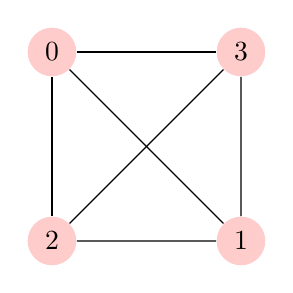
\begin{tikzpicture}
  [scale=.6,auto=left,every node/.style={circle,fill=red!20}]
  \node (n1) at (0,0) {0};
  \node (n2) at (4,-4)  {1};
  \node (n3) at (0,-4)  {2};
   \node (n4) at (4,0)  {3};

  \foreach \from/\to in { n1/n2,n1/n3,n1/n4,n2/n3,n2/n4,n3/n4}
    \draw (\from) -- (\to);

\end{tikzpicture}
\caption{A graph with 4 vertices and 6 edges}\label{1g1}
\end{center}
\end{figure}
\begin{newpage}
\end{newpage}

In our next example [Figure \ref{1g2}], we have five vertices, representing five persons, Bob, William, James, Chris and Ajur. The edges in the graph represent friendship. Chris is friends with William, James and Ajur. Bob is friends with William and James. This is depicted as a graph in Figure 1.2. It has 5 vertices and 5 edges.
\begin{figure}
\begin{center}
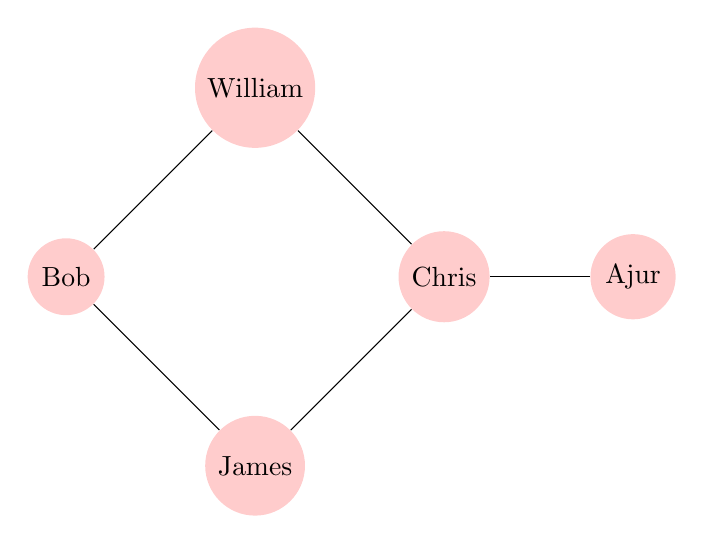
\begin{tikzpicture}
  [scale=.6,auto=left,every node/.style={circle,fill=red!20}]
  \node (n1) at (0,0) {Bob};
  \node (n2) at (4,4)  {William};
  \node (n3) at (4,-4)  {James};
   \node (n4) at (8,0)  {Chris};
    \node (n5) at (12,0) {Ajur};
  \foreach \from/\to in { n1/n2,n1/n3,n3/n4,n2/n4,n4/n5}
    \draw (\from) -- (\to);

\end{tikzpicture}
\caption{A friendship graph with 5 vertices and 5 edges}\label{1g2}
\end{center}
\end{figure}
\begin{newpage}
\end{newpage}
In our third example [Figure 1.3], we have seven Northeastern states in the United States, namely NY (New York), CT (Connecticut), VT (Vermont), ME (Maine), MA (Massachusetts) RI (Rhode Island) and NH (New Hampshire). The relationship represented is sharing a border with another state. NY borders CT, VT, and MA. CT additionally borders RI and MA. VT borders MA and NH. ME borders NH. MA borders RI and NH. This is depicted in Figure \ref{1g3}. It has 7 vertices and 10 edges.

\begin{figure}
\begin{center}
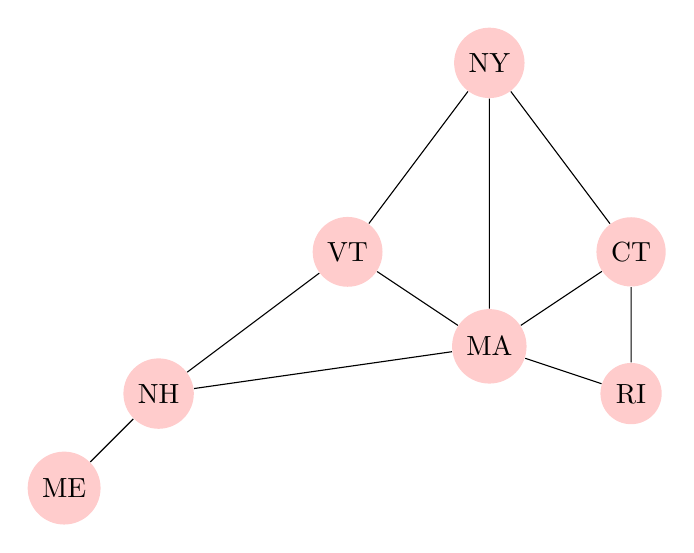
\begin{tikzpicture}
  [scale=.6,auto=left,every node/.style={circle,fill=red!20}]
  \node (n1) at (0,-6) {ME};
  \node (n2) at (2,-4)  {NH};
  \node (n3) at (6,-1)  {VT};
   \node (n4) at (9, -3) {MA};
   \node (n5) at (9,3)  {NY};
    \node (n6) at (12,-1) {CT};
    \node (n7) at (12, -4) {RI};
  \foreach \from/\to in { n1/n2,n2/n3,n2/n4, n3/n4,n3/n5,n4/n5,n4/n6,n4/n7,n5/n6,n6/n7}
    \draw (\from) -- (\to);

\end{tikzpicture}
\caption{A graph representing the northeastern United States, with 7 vertices and 10 edges}\label{1g3}
\end{center}
\end{figure}
\begin{newpage}
\end{newpage}

If there is an edge between two vertices (like NY and VT in Figure 1.3), we say that these two vertices are \textbf{adjacent}. For instance, NY is adjacent to VT and VT is adjacent to NY.

%\chapter{Introduction}
   

\chapter{Trip to the Cemetery}
It was a Halloween, a cold and dreary evening. Ajur was interested in visiting the famous cemetery in Royt as any teenager with an adventurous spirit would be. His pet dog Jura, a Labrador, was eager to follow him. As Ajur was examining the headstones and tombs, he lost track of time and it was getting dark. He grew tired and he and Jura sat under a tree and they fell asleep. Suddenly they were awakened by a loud noise. The noise was from Rishnak, a ghost who lived in the cemetery. Rishnak had died a few years ago; he used to teach mathematics and graph theory for talented high school students in the area. When Rishnak spotted Ajur in that cemetery, he thought to himself, ``here is an unusual teenager." Perhaps he could test whether this youngster  was proficient in mathematics. If he was indeed proficient, Rishnak could reward him with his magical powers. When Rishnak appeared in front of Ajur, Jura started barking.  

Rishnak was afraid he would intimidate Ajur by being brusque. Jura was barking very loudly. So Rishnak started talking in a soft voice. He gently asked what grade Ajur was in. Ajur replied that he was in middle school and studying in 8th grade. Rishank proceeded to ask the boy what subjects he liked most in school. Ajur proudly added that he was very good in mathematics. Rishnak smiled to himself. He told the boy that he had been cursed to live as ghost and his curse would be lifted if he could reward some youngsters who could answer all his questions. Ajur was intrigued by Rishnak's offer and he jumped at the possibility of rewards, and the opportunity to help lift the curse on Rishnak, a ghost, and tell his friends about his adventure.
\chapter{Degrees}
Rishnak asked Ajur whether he knew about graphs and trees in mathematics. Ajur jumped up and down and proclaimed that he knew all about graph theory. He continued that graphs are often used to  represent relations of a set of objects. He enthusiastically stated that the famous mathematician Euler was the father of graph theory. He was eager to show off his knowledge and described the famous  K\"{o}nigsberg bridge problem.  K\"{o}nigsberg (in modern day Russia) was on the banks of the Pregel river.  There were seven bridges across this river, connecting the two sides of the river and two islands. Ajur drew a graph of this on a piece of paper he was carrying.
\begin{figure}
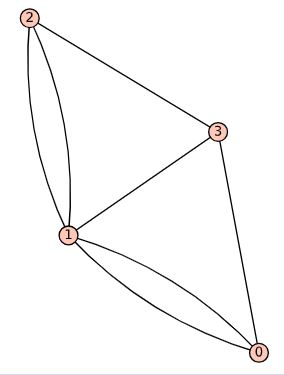
\includegraphics[width=0.6\textwidth]{konigsberg.JPG}
\caption{A Graph representing K\"{o}nigsberg Bridge. Vertices 1 and 3 are islands and 0 and 2 are the two riverbanks.}\label{kon}
\end{figure}

He continued that the problem was to start from the vertex labeled 0 and go through all bridges once and only once and return to the starting vertex 0. Ajur could not contain his enthusiasm and asked Rishnak how to do it. Rishnak gently reminded Ajur that he was the one asking questions and Ajur just had to respond with correct responses. Ajur nodded his head enthusiastically.

 Since this was the first time, Rishnak told Ajur that he was going to ask Ajur a series of questions and observe whether his curses could be lifted.
 
 Rishnak then asked Ajur, ``in a class of 33 students, what is the maximum and minimum number of friends a student can have?"\footnote{Being friend is a mutual relation, i.e. if A is a friend of B, then B is a friend of A. A student cannot be a friend to herself!}
 
 Ajur nonchalantly replied that the maximum number is 32 and the minimum number is 0.
 
 Rishnak then asked Ajur ``will there be a student in a class having 32 friends and a student having 0 friends?"
 
 Ajur smiled to himself that Rishnak seems like a clever ghost; Ajur replied, ``how is that possible --- if a student has 32 friends, so she is friends with everyone else, then everyone else has at least one friend. 
 So there cannot be a 
 student with 0 friends. Similarly if there is a student with 0 friends, there are only 32 students remaining and another student can have at most 31 friends."
 
 Rishnak was pleased to have found someone who seemed to have the ability to help him and the questioning continued. ``Can all the 33 students have a distinct number of friends?"
 
 Ajur responded immediately saying it is not possible because there are 33 distinct students, and the distinct number of friends the class can have is $\{0,1,2,\cdots,32\}$. There are 33 numbers in this, but alas it contains both students with 32 friends and with 0 friends. Ajur just had told Rishnak that it is not possible to have a student with 32 friends and another student with 0 friends.
 
 Rishnak asked Ajur, ``can there be just two students having the same number of friends, with the others all having distinct numbers of friends?" Rishnak further added that all of the students have at least one friend.
 
Ajur wanted to reason it out. He knew that the maximum number can only be 32, and the minimum has to be 1, so there are 32 distinct numbers. But there are 33 students. So by the pigeon hole principle --- if there are more pigeons than boxes, then one box contains at least two pigeons --- there have to be two students with the same number of friends.  He then reasoned about what the numbers could be. He matched 32 with 1: that is, the student having one friend has to be a friend of a student with 32 friends. Then he matched 2 with 31: the student with 2 friends has to be a friend of a student with 32 friends and a student with 31 friends. Continuing this argument, he matched 3 with 30, 4 with 29, $\cdots$, 15 with 18 and 16 with 17. We have an even number of students accounted for but an odd number of total students. That means there are two students having the same number of friends.

Rishnak posed the next question: He asked 5 students in a class of 6 students how many friends each of them have and they all gave distinct numbers greater than 0. How many friends does the student who was not asked have?

Ajur thought about this. If all the five students had given distinct numbers and they were greater than 0, they had to be $\{1,2,3,4,5\}$. Let the students be A(pu), B(art), C(arla), D(uma), E(rnie) having 5, 4, 3, 2 and 1 friends respectively. Let F(orme) be the sixth student. A is friends with B, C, D, E and F. B is friends with C, D and F. B is already friends with A and E has only one friend, namely A. Now C is friends with F. C is already friends with A and B, and D and E have their friends quota counted already. 
Now it is easy to see that F(orme) has exactly 3 friends, namely A, B and C.

Ajur drew the following graph as in Figure 3.2

\begin{figure}
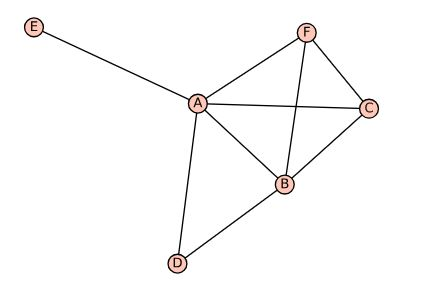
\includegraphics[width=0.6\textwidth]{graphstory1-1.JPG}
\caption{A Graph with 6 students and 5 students having 5, 4, 3, 2 and 1 friends}
\end{figure}

Rishnak was impressed, but wanted to test Ajur further. He asked whether there can an be odd number of students having odd number of friends. Ajur said that it is impossible as the sum of all numbers of friends across all students has to be even. He reasoned that if A is a friend of B, then this friendship is counted twice. Hence the sum of all friends of students is even. We know that the students having an even number of friends will contribute an even number of friendships. This in turn implies that the number of students having an odd number of friends has to be even.


Rishnak started asking, ``can you draw a graph of a class with 5 students respectively having 1, 2, 2, 2 and 1 friends?"

Ajur whipped up the graph drawn in Figure 3.3. 

\begin{figure}
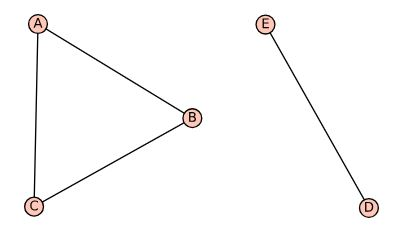
\includegraphics[width=0.6\textwidth]{graphstory1-2.JPG}
\caption{A Graph with 5 students having 2, 2, 2, 1 and 1 friends}
\end{figure}

Rishnak asked whether one can draw another graph having the given friends list.\footnote{Hakimi has given a method of constructing a graph with a given degree sequence}

Ajur took no time to respond and drew another graph as in Figure 3.4.

\begin{figure}
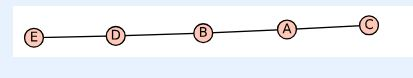
\includegraphics[width=0.6\textwidth]{graphstory1-3.JPG}
\caption{Another Graph with 5 students having 2, 2, 2, 1 and 1 friends}
\end{figure}

Jura was waking up and wanted to play with Ajur. Rishnak was happy to see the answers that Ajur gave. He saw a ray of hope that his curse could be lifted. 

Rishnak told Ajur to come back the next night, and he disappeared in a cold mist.
%\chapter{Puzzle 2}
\chapter{Rooted Trees and Trees}

Rishnak found Ajur and his dog Jura walking along a row of graves. Ajur was reading the inscriptions on the tombstones. Each headstone had the names of the family (parents, wife, husband) and the dates of birth and of death. Ajur did not know so many relatives could be buried in such a small area. He then thought of how different cultures honor their departed ones \footnote{He remembered seeing the movie Coco in 2017 about how people in Mexico remember their departed ones. He had also heard how Hindus in India go to the city of Banaras/Varanasi to perform rituals to thank and honor their deceased forefathers.} 
Ajur remembered the definition of a tree and a rooted tree. He was talking to Jura, saying that a rooted tree in graph theory/mathematics looks like a normal tree with a distinguished vertex. A rooted tree in real life has a root at the bottom whereas a rooted tree in graph theory is drawn with a root at the top. Both of them convey the same information.

``Here are two drawings of the same information." Ajur further explained that each vertex in a rooted tree has just one parent vertex (except the root vertex which has no parent). A rooted tree can also be thought of as a graph with a collection of vertices and edges. There are some restrictions. But that will become clearer, as the story proceeds.


\begin{figure}
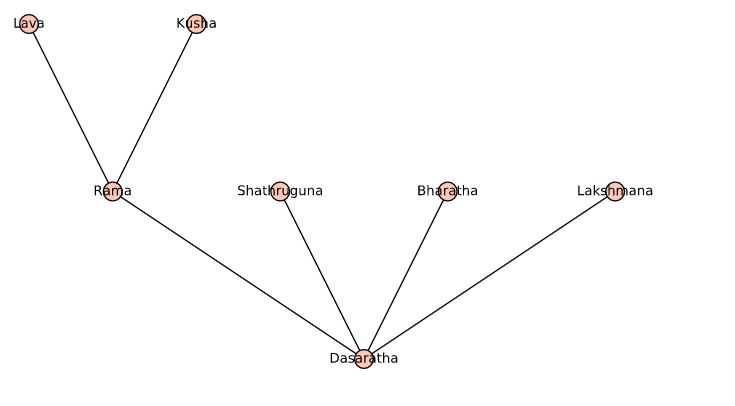
\includegraphics[width=\textwidth]{tree1.JPG}
\caption{A Tree drawn with a root at the bottom}
\end{figure}

\begin{figure}
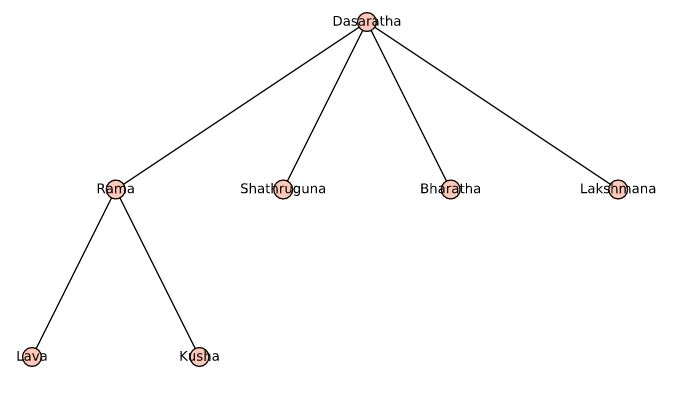
\includegraphics[width=\textwidth]{tree2.JPG}
\caption{Same Tree drawn with a root at the top}
\end{figure}

Rishnak caught up with Ajur and Jura as he had been following them quietly. Rishnak asked Ajur: ``how many edges does a rooted tree with 7 vertices have?" Ajur reasoned that since each vertex other than the root has exactly one parent vertex and there are no other edges, then number of edges will be 6. Rishnak then asked how many edges a rooted tree with 1000 vertices has. Ajur shot back with his answer 999. Impressed, but not unduly, Rishnak asked how many edges there are in a rooted tree with $n$ vertices. Nonchalantly, Ajur replied it is $n-1$ by the same argument (each of the $n-1$ vertices have just one edge connected to its parent).  

For each vertex other than a root vertex, there is a parent vertex and zero or more child vertices.  The descendants of a vertex are all its children, grandchildren, great grandchildren vertices etc. Analogously, for each vertex the ancestors of that vertex are its parent, grandparent, great grandparent vertices etc. 
A vertex with no child vertices is known as a leaf vertex. Rishnak asked Ajur ``what is the largest number of leaf vertices a tree with 6 vertices can have?" Ajur immediately responded that the number is 5, and he drew a rooted tree as in Figure \ref{t1}.

\begin{figure}
\begin{center}
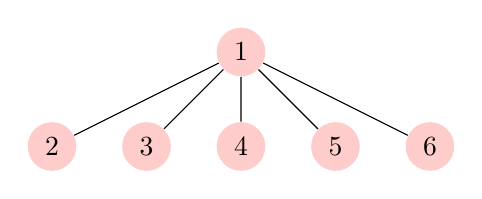
\begin{tikzpicture}
  [scale=.6,auto=left,every node/.style={circle,fill=red!20}]
  \node (n6) at (5,5) {1};
  \node (n4) at (1,3)  {2};
  \node (n5) at (3,3)  {3};
  \node (n1) at (5,3) {4};
  \node (n2) at (7,3)  {5};
  \node (n3) at (9,3)  {6};

  \foreach \from/\to in {n6/n1,n6/n2,n6/n3,n6/n4,n6/n5}
    \draw (\from) -- (\to);

\end{tikzpicture}

\caption{A Tree with 6 vertices and 5 leaf vertices. The vertex labeled 1 is the root vertex}\label{t1}
\end{center}
\end{figure}

Rishnak asked, ``what is the smallest number of leaf vertices a tree with 6 vertices can have?" Ajur knew this answer too. So he drew a rooted tree as in Figure~\ref{t2}.

\begin{figure}
\begin{center}
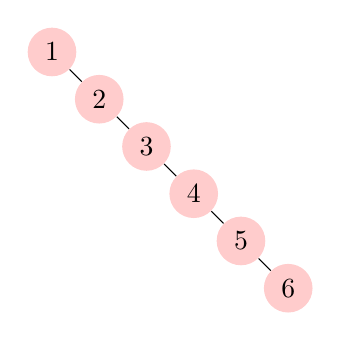
\begin{tikzpicture}
  [scale=.6,auto=left,every node/.style={circle,fill=red!20}]
  \node (n6) at (3,7) {1};
  \node (n4) at (4,6)  {2};
  \node (n5) at (5,5)  {3};
  \node (n1) at (6,4) {4};
  \node (n2) at (7,3)  {5};
  \node (n3) at (8,2)  {6};

  \foreach \from/\to in {n6/n4,n4/n5,n5/n1,n1/n2,n2/n3}
    \draw (\from) -- (\to);

\end{tikzpicture}

\caption{A Tree with 6 vertices and one leaf vertex labeled 6. The vertex labeled 1 is the root vertex.}\label{t2}
\end{center}
\end{figure}

Rishnak said ``We get a lot of lightning and thunderstorms here, especially during summer months. Lightning affects tall objects, especially objects that conduct electricity in an open area\footnote{Benjamin Franklin had demonstrated the electrical nature of lightning}. Lightning conductors are usually at the top of the buildings and have less resistance than the building, and hence lightning passes through the conductor." Rishnak drew a rooted tree with 3 vertices as shown in Figure~\ref{t3}.

\begin{figure}
\begin{center}

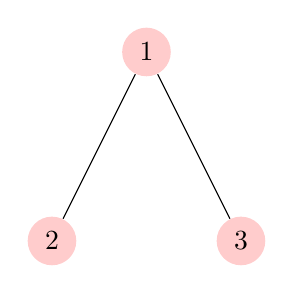
\begin{tikzpicture}
  [scale=.6,auto=left,every node/.style={circle,fill=red!20}]
  \node (n1) at (3,7) {1};
  \node (n2) at (1,3)  {2};
  \node (n3) at (5,3)  {3};


  \foreach \from/\to in {n1/n2,n1/n3}
    \draw (\from) -- (\to);

\end{tikzpicture}

\caption{A resistance  Tree with 3 vertices and two leaf vertices at the ground. }\label{t3}
\end{center}
\end{figure}


Rishnak said that the each edge has a resistance of 1 ohm, and vertices labeled 2 and 3 are grounded. What is the effective resistance of the resistance tree in Figure~\ref{t3}? Ajur remembered his physics and he realized two resistances are in parallel. So he immediately replied that the effective resistance is $\frac{1}{2}$ ohms. (Intuitively, there are two paths the current can take and hence the resistance splits evenly between the 2 paths).

Rishnak asked the same question, effective resistance, for the following rooted tree shown in Figure \ref{t4}.
\begin{figure}
\begin{center}

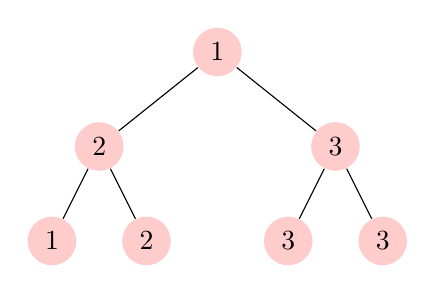
\begin{tikzpicture}
  [scale=.6,auto=left,every node/.style={circle,fill=red!20}]
  \node (n1) at (5.5,7) {1};
  \node (n2) at (3,5)  {2};
  \node (n3) at (8,5)  {3};
  \node (n4) at (2,3) {1};
  \node (n5) at (4,3)  {2};
  \node (n6) at (7,3)  {3};
  \node (n7) at (9,3)  {3};

  \foreach \from/\to in {n1/n2,n1/n3,n2/n4,n2/n5,n3/n6,n3/n7}
    \draw (\from) -- (\to);

\end{tikzpicture}

\caption{A resistance  Tree with 7 vertices and four leaf vertices at the ground. }\label{t4}
\end{center}
\end{figure}

Ajur said that he had computed the effective resistances for trees rooted at vertex labeled 2 and 3 to be $\frac{1}{2}$. There are two parallel paths with equal resistance of $1+\frac{1}{2}$ (There is a series connection from root vertex 1 and vertices labeled 2 and 3 respectively). Hence the effective resistance is $\frac{3}{4}$ ohms. Ajur further said that there is a pattern here. For the resistance tree with 15 vertices (adding one more level or increasing the height), the effective resistance will be $\frac{7}{8}$. Rishnak then asked what happens if the tree is of infinite height! (A really tall lightning conductor.) Ajur was perplexed - But then he reasoned that this could be formulated as a recurrence relation. Let R be the effective resistance of this infinite tree. The root has two children, each of which will have a resistance of R ohms. The root vertex is connected to the child vertex with a resistance of 1 ohm. Hence he wrote an equation $$R= \frac{R+1}{2}$$ Simplifying this, he got the resistance of 1 ohm. A really tall lightning conductor (a tree of infinite height) with a very low resistance - hence an excellent lightning conductor.\footnote{Because of a large number of joints, this solution may not be a practical one!} Rishnak responded that there is another way of getting the same result. From an earlier example, you can generalize the resistance to be $\frac{2^h-1}{2^h}$ , $h$ being height (longest among path lengths from the root vertex to all leaf vertices) of the rooted tree. This can be further simplified to be $1-\frac{1}{2^h}$. As $h$ goes to infinity the term $\frac{1}{2^h}$ goes to 0 and hence the resistance is 1. Ajur learned an important lesson that there are multiple ways of getting a solution and each one may provide a new insight. Ajur asked Rishnak: ``can you construct an infinite height tree (with edge resistances being one ohm) so that the effective resistance is $\frac{1}{2}$, $\frac{1}{3}$, $\frac{1}{4}$ or more generally any fraction $\leq$~1?" Rishnak replied to Ajur that he was the one who could ask questions and not Ajur.\footnote{Of course Rishnak knew the answer and suggests others to think every vertex having more than 2 child vertices!}

A tree is like a rooted tree but with no root vertex. A tree can be drawn in any manner. The degree of a vertex is the number of edges incident on that vertex. The leaf (pendant) vertex has a degree of 1. So in Figure~\ref{t2} both vertices labeled 1 and 6 are leaf/pendant vertices and all other vertices have degree 2. 

Rishnak told Ajur that one important property of a tree is that there are no cycles in it. Ajur could easily understand it from a genealogy perspective - a person cannot be an ancestor as well as a descendant of himself/herself.  Ajur added that there is only one path between any two vertices in a tree (Of course, Ajur assumed that the edges are undirected --- which Rishnak knew). Rishnak asked ``how did you infer that there is a unique path between two vertices in a tree?" Ajur promptly replied that if there are two paths between any two vertices, there will be a cycle (which cannot exist in a tree). Since there is an unique path between two vertices, one can compute the distance between two vertices as the number of edges in that path. Ajur provided clarifications with examples.  As an example in Figure~\ref{t1}, the distance between the vertex labeled 1 and any other vertex is 1. The distance between the vertex labeled 2 and the vertex labeled 6 is 2. In Figure~\ref{t2}, the distance between the vertex labeled 1 and the vertex labeled 6 is 5 and the distance between the vertex labeled 2 and the vertex labeled 4 is 2.
%(Dad: you could also add the fact that every finite tree has a center of mass! it's in this vein, and not especially well known (Boris hadn't realized it!))
\chapter{Subgraphs}
Rishnak found Ajur sleeping with his dog Jura near the cemetery and saw a headstone nearby with the name Schossow. Rishnak recognized the name  from Instant Insanity Puzzle{\footnote{It is also known as Katzenjammer, (Great) Tantalizer, Face-4, Cube-4, Bognar Balls, Taktikolor, Frantic, Diabolical, Damblocks,
Symington's Puzzle. A patent was awarded to  Schossow in 1990}}. Just as Rishnak was thinking it would be an interesting topic to discuss with Ajur, Jura the dog, eager to explore, nudged Ajur. Before long, Ajur and Jura were strolling along a path where Rishnak startled Ajur (as ghosts tend to do). 

Rishnak asked Ajur what he knew about subgraphs. Ajur said that he was familiar with subsets. Since a graph has both a vertex set and edge set, he can deduce what a subgraph is. If a graph $G=(V,E)$ with a vertex set $V$ and an edge set $E$, then take any subset $X$ of $V$ and consider all the edges in E, which has both its end vertices in $X$. Ajur drew this.
\vspace{0.2in}
\\
\noindent
\begin{figure}
\begin{center}
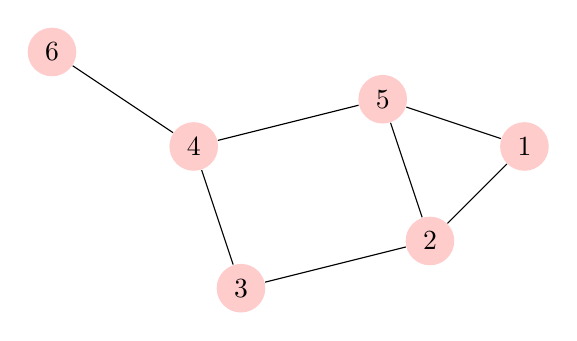
\begin{tikzpicture}
  [scale=.6,auto=left,every node/.style={circle,fill=red!20}]
  \node (n6) at (1,10) {6};
  \node (n4) at (4,8)  {4};
  \node (n5) at (8,9)  {5};
  \node (n1) at (11,8) {1};
  \node (n2) at (9,6)  {2};
  \node (n3) at (5,5)  {3};

  \foreach \from/\to in {n6/n4,n4/n5,n5/n1,n1/n2,n2/n5,n2/n3,n3/n4}
    \draw (\from) -- (\to);

\end{tikzpicture}
\caption{ Example Graph with 6 vertices and 7 edges}\label{3g}
\end{center}
\end{figure}
\\
\noindent
If one took a vertex subset $\{1,2,3,5\}$ of Figure \ref{3g} the subgraph could be as in Figure \ref{3g1}.
\begin{figure}
\begin{center}
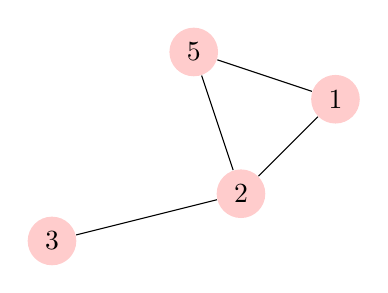
\begin{tikzpicture}
  [scale=.6,auto=left,every node/.style={circle,fill=red!20}]
  %\node (n6) at (1,10) {6};
  %\node (n4) at (4,8)  {4};
  \node (n5) at (8,9)  {5};
  \node (n1) at (11,8) {1};
  \node (n2) at (9,6)  {2};
  \node (n3) at (5,5)  {3};

  \foreach \from/\to in {n5/n1,n1/n2,n2/n5,n2/n3}
    \draw (\from) -- (\to);
\end{tikzpicture}
\caption{Induced Subraph of Figure \ref{3g} Vertices 1,2,3 and 5 are chosen and all the edges between these vertices which are present in the original graph have to be in this subgraph}\label{3g1}
\end{center}
\end{figure}
\\
\noindent
Rishnak laughed and said that the subgraph Ajur drew was called an \textit {induced subgraph} --- that is, all the edges are included in the vertex subset. You have the flexibility of choosing only a subset of these edges. But there is one extra condition: for each edge in the chosen subset of edges, the end vertices should be in the chosen vertex subset. 
\\
\begin{figure}
\begin{center}
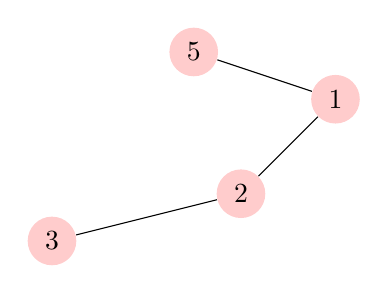
\begin{tikzpicture}
  [scale=.6,auto=left,every node/.style={circle,fill=red!20}]
  %\node (n6) at (1,10) {6};
  %\node (n4) at (4,8)  {4};
  \node (n5) at (8,9)  {5};
  \node (n1) at (11,8) {1};
  \node (n2) at (9,6)  {2};
  \node (n3) at (5,5)  {3};

  \foreach \from/\to in {n5/n1,n1/n2,n2/n3}
    \draw (\from) -- (\to);

\end{tikzpicture}
\caption{A subgraph of Figure \ref{3g}}\label{3g2}
\end{center}
\end{figure}
\\
\noindent
Rishnak illustrated this with the following subgraph example as shown in Figure \ref{3g2}. A subgraph with no vertices and no edges is also an induced subgraph (and subgraph) of any graph.


%Rishnak said that in a graph having $n$ vertices where the vertices are labeled (have a number/name associated with them), then there are at least $2^n$ subgraphs and exactly $2^n$ induced subgraphs.  There are ${n \choose i}$ ways of choosing $i$ vertices from a given set of $n$ vertices. Once the vertices are chosen, the edges are fixed for an induced subgraph. Since $i$ can vary from 0 to $n$, we get $2^n$ induced subgraphs. Since every induced subgraph is a subgraph (and not every subgraph is not an induced subgraph), we have at least $2^n$ subgraphs.  

A walk from a vertex $i$ to a vertex $j$ is an alternating sequence of vertices and edges. Every edge in that walk is incident between vertices preceding and succeeding that edge. For example in Figure \ref{3g},
a walk from vertex 6 to vertex 1 could be 6 (6,4), 4, (4,3), 3, (3,2), 2, (2,1) and 1. The edges are represented as a vertex pair. If those edges are labelled with a name, that label could be used instead. Another walk in Figure \ref{3g} from vertex 6 to vertex 1 could be 6, (6,4), 4, (4,5), 5 (5,1), 1.  The only other condition that the walk has (besides an edge being incident on a preceding and a succeeding vertex) is that all the edges have to be distinct. However the vertices in a walk can be repeated. 
Here is another example Figure \ref{3g3}. A walk from vertex 1 and vertex 8 could be 1, (1,2), 2, (2,4), 4, (4,6), 6, (6,8) and 8. (8,2), 2, (2,3), 3, (3,4), 4, (4,5), 5, (5,6), 6, (6,7), 7, (7,8) and 8. Ajur was naturally getting bored. He interjected that in your walk you have visited all the edges in the graph (shown in Figure \ref{3g3}). Ajur further added that this was similar to the K\"{o}nigsberg Bridge Problem (Figure \ref{kon} mentioned earlier in Chapter 3!).  
\begin{figure}
\begin{center}
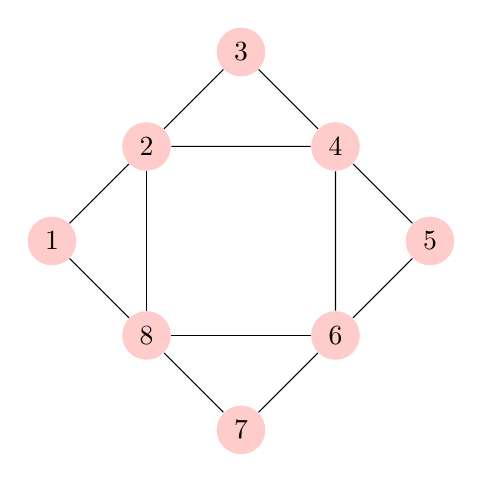
\begin{tikzpicture}
  [scale=.6,auto=left,every node/.style={circle,fill=red!20}]
  \node (n1) at (1,7) {1};
  \node (n2) at (3,9)  {2};
  \node (n3) at (5,11)  {3};
  \node (n4) at (7,9) {4};
  \node (n5) at (9,7)  {5};
  \node (n6) at (7,5)  {6};
  \node (n7) at (5,3)  {7};
  \node (n8) at (3,5)  {8};

  \foreach \from/\to in {n1/n2,n1/n8,n2/n3,n2/n4,n2/n8,n3/n4,n4/n5,n4/n6,n5/n6,n6/n7,n6/n8,n7/n8}
    \draw (\from) -- (\to);

\end{tikzpicture}
\caption{ Example Graph with 8 vertices and 12 edges}\label{3g3}
\end{center}
\end{figure}
\\

If the starting and ending vertices in a walk are the same, it is known as a closed walk. If all the edges in a closed walk are distinct, then it is known as a cycle. 
Ajur had heard of this from his friends.
Rishnak asked Ajur to list two cycles from Figure \ref{3g3}. Ajur had no trouble at all, in listing two cycles as (1,(1,2),2,(2,8),8,(8,1),1) and (2,(2,4),4,(4,6),6,(6,8),8,(8,2)2). Often the edges are omitted, and the cycles are written as (1,2,8,1) and (2,4,6,8,2).  Of course, a cycle and a walk are examples of subgraphs with some added conditions. These added conditions make the study of subgraphs very interesting. If in a cycle, all the vertices of the original graph are present, then that cycle is known as a Hamiltonian Cycle. For example in Figure \ref{3g3} the cycle (1,2,3,4,5,6,7,8,1) is a Hamiltonian Cycle of Figure \ref{3g4}. If all the edges in a walk are distinct then it is known as a path. Ajur gave the following examples for a path in Figure \ref{3g3} as (1,(1,2),2,(2,3),3) or simply as (1,2,3), Figure \ref{3g5}. If there is a path between every pair of vertices in a subgraph, then the subgraph is said to be connected. If a subgraph contains no cycles and is connected, the subgraph is a tree. If such a tree contains all vertices then it is known as spanning tree, Figure \ref{3g6}.  A subgraph in which the degree of every vertex is 1 is called a matching. An example of a subgraph (which is a matching for Figure \ref{3g3}) is in Figure \ref{3g7}. If the subgraph contains all vertices and the degree of every vertex is one, then it is called as Perfect matching. An example of a subgraph that is a perfect matching for Figure~\ref{3g3} is in Figure \ref{3g8}. Rishnak asked Ajur how many perfect matchings there are in Figure \ref{3g3}. Ajur thought a bit. He saw vertices 1, 3, 5 and 7 hae degree 2. Hence one of those incident on 1, 3, 5 and 7 have to be selected. Hence he replied that there are exactly two perfect matchings in Figure \ref{3g3}. 
\\
\begin{figure}
\begin{center}
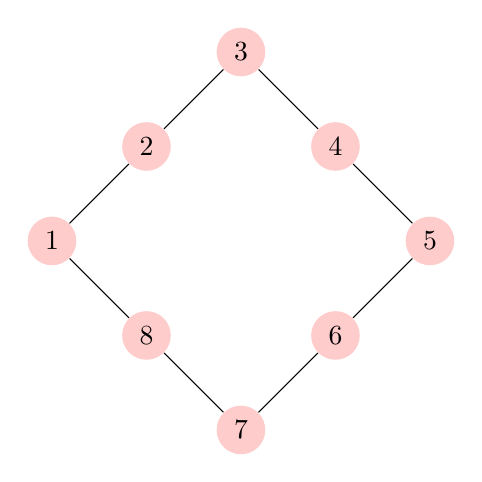
\begin{tikzpicture}
  [scale=.6,auto=left,every node/.style={circle,fill=red!20}]
  \node (n1) at (1,7) {1};
  \node (n2) at (3,9)  {2};
  \node (n3) at (5,11)  {3};
  \node (n4) at (7,9) {4};
  \node (n5) at (9,7)  {5};
  \node (n6) at (7,5)  {6};
  \node (n7) at (5,3)  {7};
  \node (n8) at (3,5)  {8};

  \foreach \from/\to in {n1/n2,n1/n8,n2/n3,n3/n4,n4/n5,n5/n6,n6/n7,n7/n8}
    \draw (\from) -- (\to);

\end{tikzpicture}
\caption{ A subgraph which is a Hamiltonian Cycle}\label{3g4}
\end{center}
\end{figure}

\begin{figure}
\begin{center}
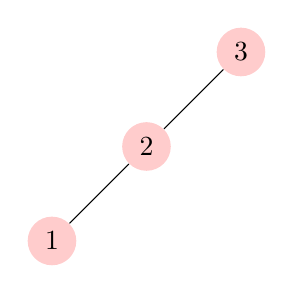
\begin{tikzpicture}
  [scale=.6,auto=left,every node/.style={circle,fill=red!20}]
  \node (n1) at (1,7) {1};
  \node (n2) at (3,9)  {2};
  \node (n3) at (5,11)  {3};


  \foreach \from/\to in {n1/n2,n2/n3}
    \draw (\from) -- (\to);

\end{tikzpicture}
\caption{ A subgraph which is a tree}\label{3g5}
\end{center}
\end{figure}

\begin{figure}
\begin{center}
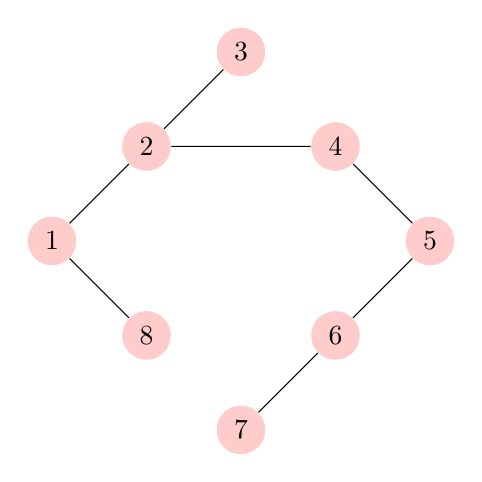
\begin{tikzpicture}
  [scale=.6,auto=left,every node/.style={circle,fill=red!20}]
  \node (n1) at (1,7) {1};
  \node (n2) at (3,9)  {2};
  \node (n3) at (5,11)  {3};
  \node (n4) at (7,9) {4};
  \node (n5) at (9,7)  {5};
  \node (n6) at (7,5)  {6};
  \node (n7) at (5,3)  {7};
  \node (n8) at (3,5)  {8};

  \foreach \from/\to in {n1/n2,n1/n8,n2/n3,n2/n4,n4/n5,n5/n6,n6/n7}
    \draw (\from) -- (\to);

\end{tikzpicture}
\caption{ A subgraph which is a spanning tree}\label{3g6}
\end{center}
\end{figure}

\begin{figure}
\begin{center}
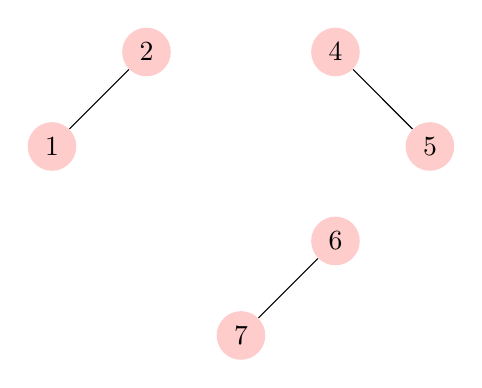
\begin{tikzpicture}
  [scale=.6,auto=left,every node/.style={circle,fill=red!20}]
  \node (n1) at (1,7) {1};
  \node (n2) at (3,9)  {2};
  %\node (n3) at (5,11)  {3};
  \node (n4) at (7,9) {4};
  \node (n5) at (9,7)  {5};
  \node (n6) at (7,5)  {6};
  \node (n7) at (5,3)  {7};
  %\node (n8) at (3,5)  {8};

  \foreach \from/\to in {n1/n2,n4/n5,n6/n7}
    \draw (\from) -- (\to);

\end{tikzpicture}
\caption{ A subgraph which is a matching}\label{3g7}
\end{center}
\end{figure}

\begin{figure}
\begin{center}
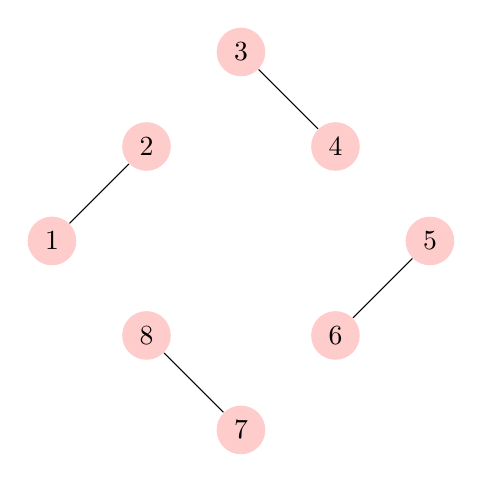
\begin{tikzpicture}
  [scale=.6,auto=left,every node/.style={circle,fill=red!20}]
  \node (n1) at (1,7) {1};
  \node (n2) at (3,9)  {2};
  \node (n3) at (5,11)  {3};
  \node (n4) at (7,9) {4};
  \node (n5) at (9,7)  {5};
  \node (n6) at (7,5)  {6};
  \node (n7) at (5,3)  {7};
  \node (n8) at (3,5)  {8};

  \foreach \from/\to in {n1/n2,n3/n4,n5/n6,n7/n8}
    \draw (\from) -- (\to);

\end{tikzpicture}
\caption{ A subgraph which is a perfect matching}\label{3g8}
\end{center}
\end{figure}

\vspace{3in}
A graph is connected if there is a path between every pair of vertices in that graph. Otherwise the graph is disconnected,  Here is an example of a connected graph, Figure \ref{3g9}. Here is an example of a graph that is not connected, Figure \ref{3g10}
\begin{figure}
\begin{center}
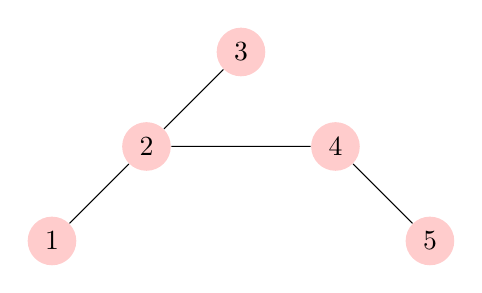
\begin{tikzpicture}
  [scale=.6,auto=left,every node/.style={circle,fill=red!20}]
  \node (n1) at (1,7) {1};
  \node (n2) at (3,9)  {2};
  \node (n3) at (5,11)  {3};
  \node (n4) at (7,9) {4};
  \node (n5) at (9,7)  {5};
\foreach \from/\to in {n1/n2,n2/n3,n2/n4,n4/n5}
    \draw (\from) -- (\to);

\end{tikzpicture}
\caption{ A connected graph}\label{3g9}
\end{center}
\end{figure}

\begin{figure}
\begin{center}
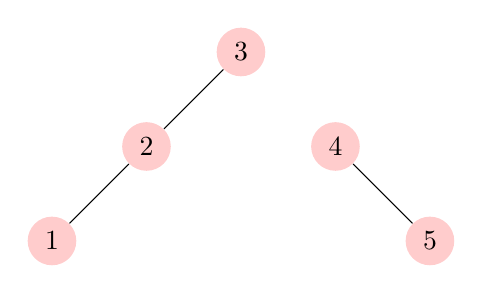
\begin{tikzpicture}
  [scale=.6,auto=left,every node/.style={circle,fill=red!20}]
  \node (n1) at (1,7) {1};
  \node (n2) at (3,9)  {2};
  \node (n3) at (5,11)  {3};
  \node (n4) at (7,9) {4};
  \node (n5) at (9,7)  {5};
\foreach \from/\to in {n1/n2,n2/n3,n4/n5}
    \draw (\from) -- (\to);

\end{tikzpicture}
\caption{ A graph that is not connected}\label{3g10}
\end{center}
\end{figure}
\vspace{3in}

\textbf{Question for the third day:} Rishnak asked Ajur to list the cycles in the following graph Figure \ref{day3g1} 

\begin{figure}
\begin{center}
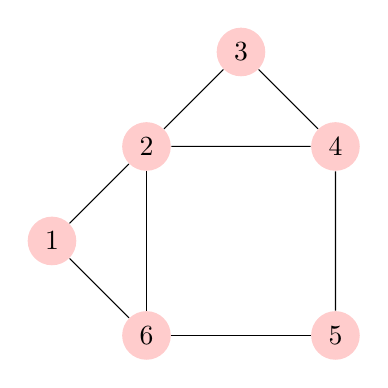
\begin{tikzpicture}
  [scale=.6,auto=left,every node/.style={circle,fill=red!20}]
  \node (n1) at (1,7) {1};
  \node (n2) at (3,9)  {2};
  \node (n3) at (5,11)  {3};
  \node (n4) at (7,9) {4};
  \node (n5) at (7,5)  {5};
  \node (n6) at (3,5)  {6};

  \foreach \from/\to in {n1/n2,n1/n6,n2/n3,n2/n4,n2/n6,n3/n4,n4/n5,n5/n6}
    \draw (\from) -- (\to);

\end{tikzpicture}
\caption{ How many Cycles are there in this Graph?}\label{day3g1}
\end{center}
\end{figure}

\textbf{Answer:} Ajur listed the 6 cycles as follows:
\begin{enumerate}
    \item Cycle of length 3 (two namely  (1,2,6), (2,3,4)
    \item Cycle of length 4 (one namely) (2,4,5,6)
    \item Cycle of length 5 (two namely) (2,3,4,5,6), (1,2,4,5,6)
    \item Cycle of length 6 (one namely) (1,2,3,4,5,6)
\end{enumerate}
Rishnak  was pleased and noticed that Ajur was getting restless, and so was Jura, and so they called it a day.
\chapter{Euler Paths/Cycles}

Ajur was tired after listening to a lot of definitions and examples. He complained to Jura that looked too much like a Math class and he preferred fun Math problems instead. As Ajur was mentioning, Rishnak was overhearing this conversation. Rishnak too felt that the pprvious day's conversation was very cut and dry. His ghost friends were accusing of making the beautiful subject of Graph Theory dull and monotnous.


An Euler walk of a connected graph is a walk that includes every edge exactly once. If the starting vertex and the ending vertex are the same then it is called a closed Euler walk. Of course the name Euler comes from 
Rishnak decided to take on the oldest problem on Graph Theory Euler walk and closed Euler walk. Rishnak caught up with Ajur and Jura walking along a desolate road. Rishnak asked Ajur in the Figure \ref{4g1} whether there is a walk starting from vertex 2 to vertex 4 passing all the edges exactly once [This is what is known as an Eulerian walk]. Ajur saw there is a cycle (2,3,4,1,2). After this cycle, there is just one edge (2,4) left. Hence Ajur constructed an Eulerian walk by combining the two as (2,(2,3),3,(3,4),4,(4,1),1,(1,2),2,(2,4),4) or written simply as (2,3,4,1,2,3) by omitting the edges. Ajur illustrated this Figure \ref{4g15} Ajur further added that there is no closed Eulerian walk as that would imply that the edges have to be split into cycles (with no edges in common among the cycles). This will mean that the degrees of every vertex has to be even. Rishnak was much impressed with Ajur's reasoning. 


\begin{figure}
\begin{center}
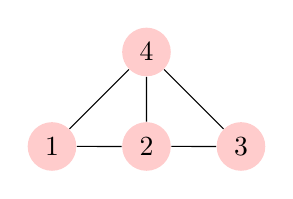
\begin{tikzpicture}
  [scale=.6,auto=left,every node/.style={circle,fill=red!20}]
  \node (n1) at (1,7) {1};
  \node (n2) at (3,7)  {2};
  \node (n3) at (5,7)  {3};
  \node (n4) at (3,9)  {4};

  \foreach \from/\to in {n1/n2,n2/n3,n2/n4,n1/n4,n3/n4}
    \draw (\from) -- (\to);

\end{tikzpicture}
\caption{ Example Graph with 4 vertices and 5 edges}\label{4g1}
\end{center}
\end{figure}

\begin{figure}
\begin{center}
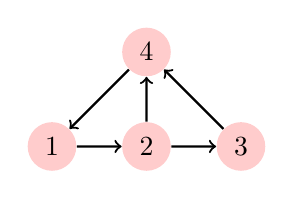
\begin{tikzpicture}
  [scale=.6,auto=left,every node/.style={circle,fill=red!20}]
  \node (n1) at (1,7) {1};
  \node (n2) at (3,7)  {2};
  \node (n3) at (5,7)  {3};
  \node (n4) at (3,9)  {4};

\path [->,draw,thick]
(n2) edge  (n3)
(n3) edge   (n4)
(n4) edge   (n1)
(n1) edge   (n2)
(n2) edge  (n4)
;
\end{tikzpicture}
\caption{ Eulerian Path from vertex 2 to vertex 4 2-3-4-1-2-4 of Figure \ref{4g1}}\label{4g15}
\end{center}
\end{figure}
\vspace{2cm}
Rishnak then asked Ajur whether you can start a walk from vertex 1 to vertex 9 and visit all edges once and only once (Eulerian walk from vertex 1 to vertex 9) in connected graph in Figure \ref{4g2}.
Ajur was perplexed. Then he tried to reason - he can break them into cycles. (2,3,7),(7,6,5,4), (3,4,8)  - None of these cycles had any edge in common. So he constructed a 
walk as (1,(1,2),2,(2,3),3,(3,4),4,(4,8),8,(8,3),3,(3,7),7, (7,6),6,(6,5),5,(5,4).4,(4,7),7,(7,2),2,(2,8),8,(8,9),9). Ajur further explained that he obtained this Eulerian walk by essentially by combining these cycles. He illustrated his walk in \ref{4g25}. Ajur responded that there is no closed Eulerian walk in this graph \ref{4g2} as all the vertices are not of even degree. An Eulerian walk startes from a vertex with odd degree and ends at a vertex with odd degree (There has tyo be exactly two vertices .

\begin{figure}
\begin{center}
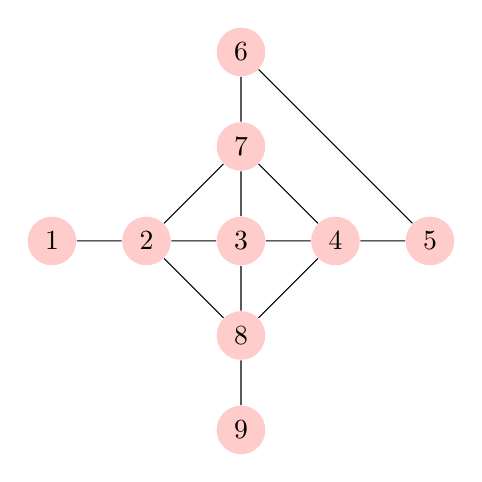
\begin{tikzpicture}
  [scale=.6,auto=left,every node/.style={circle,fill=red!20}]
  \node (n1) at (1,7) {1};
  \node (n2) at (3,7)  {2};
  \node (n3) at (5,7)  {3};
  \node (n4) at (7,7) {4};
  \node (n5) at (9,7)  {5};
  \node (n6) at (5,11)  {6};
   \node (n7) at (5,9) {7};
   \node (n8) at (5,5) {8};
   \node (n9)  at (5,3) {9};
  \foreach \from/\to in {n1/n2,n2/n3,n3/n4,n4/n5,n6/n7,n7/n3,n3/n8,n8/n9,n2/n7,
  n4/n7,n4/n8,n8/n2,n6/n5}
    \draw (\from) -- (\to);

\end{tikzpicture}
\caption{ Example Graph with 9 vertices and 13 edges}\label{4g2}
\end{center}
\end{figure}

\begin{figure}
\begin{center}
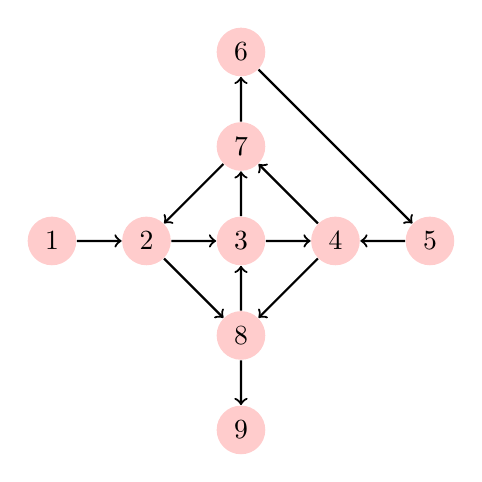
\begin{tikzpicture}
  [scale=.6,auto=left,every node/.style={circle,fill=red!20}]
  \node (n1) at (1,7) {1};
  \node (n2) at (3,7)  {2};
  \node (n3) at (5,7)  {3};
  \node (n4) at (7,7) {4};
  \node (n5) at (9,7)  {5};
  \node (n6) at (5,11)  {6};
   \node (n7) at (5,9) {7};
   \node (n8) at (5,5) {8};
   \node (n9)  at (5,3) {9};
 \path [->,draw,thick] 
  (n1) edge  (n2)
  (n2) edge (n3)
  (n3) edge (n4)
  (n4) edge (n8)
  (n8) edge (n3)
  (n3) edge (n7)
  (n7) edge (n6)
  (n6) edge (n5)
  (n5) edge (n4)
  (n4) edge (n7)
  (n7) edge (n2)
  (n2) edge (n8)
  (n8) edge (n9)
;
\end{tikzpicture}
\caption{ Eulerian Walk from vertex 1 to vertex 9  1-2-3-4-8-3-7-6-5-4-7-2-8-9 of Figure \ref{4g2}}\label{4g25}
\end{center}
\end{figure}

\vspace{3in}
Rishnak asked Ajur how would you make the graph shown in Figure \ref{4g2} to have a closed Eulerian Walk. Ajur reasoned that there are exactly two vertices of odd degrees, namely, vertices 1 and 9. If we join an edge between 1 and 9,  every vertex will have an even degree and hence a closed Eulerian Walk and that walk will be 1-2-3-4--8--7-6-5-4-7-2-8-9-1. Ajur also drew a graph.

\begin{figure}
\begin{center}
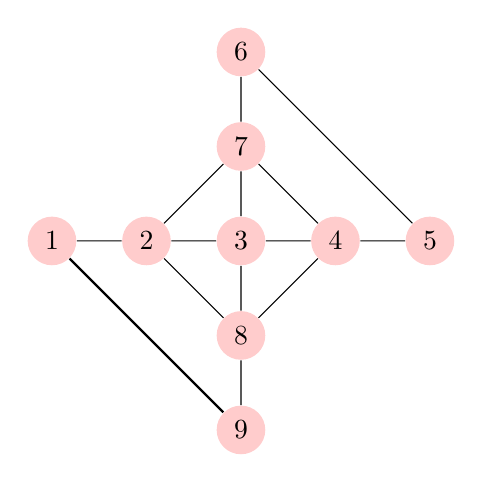
\begin{tikzpicture}
  [scale=.6,auto=left,every node/.style={circle,fill=red!20}]
  \node (n1) at (1,7) {1};
  \node (n2) at (3,7)  {2};
  \node (n3) at (5,7)  {3};
  \node (n4) at (7,7) {4};
  \node (n5) at (9,7)  {5};
  \node (n6) at (5,11)  {6};
   \node (n7) at (5,9) {7};
   \node (n8) at (5,5) {8};
   \node (n9)  at (5,3) {9};
  \foreach \from/\to in {n1/n2,n2/n3,n3/n4,n4/n5,n6/n7,n7/n3,n3/n8,n8/n9,n2/n7,
  n4/n7,n4/n8,n8/n2,n6/n5}
    \draw (\from) -- (\to);
\path[thick] (n1) edge (n9);
\end{tikzpicture}
\caption{ Closed Eulerian Walk with edge (1,9) added to Figure \ref{4g2}}\label{4g255}
\end{center}
\end{figure}

Rishnak asked how will you make graph shown in Figure \ref{4g1} to have a closed Eulerian walk. Ajur now had problem. The two vertices which have odd degrees 2 and 4, have an already an edge between them. However, he remembered the definition of a multigraph, where in between any two vertices, there can be more than one edge. So he added another edge between 2 and 4 and there is a closed Eulerian walk 2-3-4-1-2-4-2. Ajur again drew a graph as shown in Figure \ref{4g155}
Ajur added that if a graph is not connected, there is neither Eulerian walk nor a closed Eulerian walk.
\begin{figure}
\begin{center}
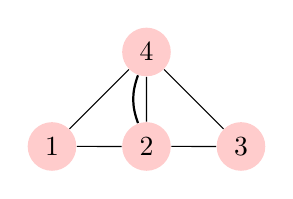
\begin{tikzpicture}
  [scale=.6,auto=left,every node/.style={circle,fill=red!20}]
  \node (n1) at (1,7) {1};
  \node (n2) at (3,7)  {2};
  \node (n3) at (5,7)  {3};
  \node (n4) at (3,9)  {4};

  \foreach \from/\to in {n1/n2,n2/n3,n2/n4,n1/n4,n3/n4}
    \draw (\from) -- (\to);
\path[thick] (n2) edge[bend left=20] (n4);
\end{tikzpicture}
\caption{ Graph in Figure \ref{4g1} with edge (2,4) added to have a closed Eulerian Walk}\label{4g155}
\end{center}
\end{figure}

\vspace{3in}
Rishnak asked Ajur whether he knew about multi graphs and directed graphs. Ajur realized he essentially learnt about multigraphs  by doing Eulerian walks and completion  example. Ajur added that in a direct an edge $(x,y)$ goes from vertex $x$ to $y$ and he drew an example graph to show Rishnak that he knows See Figure \ref{4g5}. Ajur mentioned that instead of degree of a vertex, we have in-degree and out-degree of a vertex. The number of edges coming to a vertex is the in-degree of that vertex and the number of edges going out of a vertex is the out-degree of a vertex. For example, in the directed graph shown in Figure \ref{4g5}, vertex 1 has in-degree 2 and out-degree 1, Each of Vertex 3 and 4 has in-degree  and out-degree 1. A directed graph is strongly connected if there is a directed path from every vertex to every other vertex. For example, directed graph shown in Figure \ref{4g5} is strongly connected. 
\begin{figure}
\begin{center}
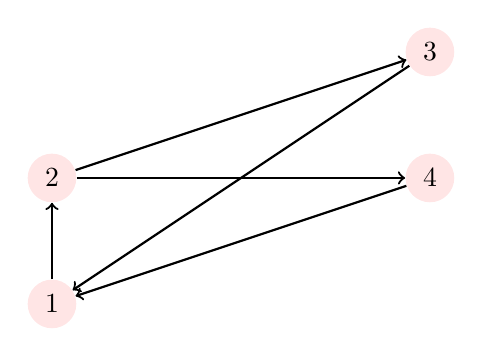
\begin{tikzpicture}
  [scale=.8,auto=left,every node/.style={circle,fill=red!10}]
  \node (n1) at (1,7) {1};
  \node (n2) at (1,9)  {2};
  \node (n3) at (7,11)  {3};
  \node (n4) at (7,9) {4};
 \path[->, draw,thick] 
        (n1) edge (n2)
         (n3) edge (n1)
        (n2) edge (n3)
        (n2) edge (n4)
        (n4) edge  (n1);

\end{tikzpicture}
\caption{ Example Directed Graph with 4 vertices and 5 edges}\label{4g5}
\end{center}
\end{figure}

Anticipating what Rishnak is going to ask, Ajur responded by saying that there is no closed Eulerian walk in this directed graph. Rishnak reminded that he wanted whether Ajur knew an Euler walk from vertex 2 to vertex 1. Ajur reasoned in a  manner similar to what he did before. Ajur saw a directed cycle (1,(1,2),2,(2,3),3,(3,1),1) or simply (1,2,3,1). So AJur was able to write the Eulerian walk as 2-3-1-2-4-1. Ajur said to have a closed Eulerian walk, you should have a collection of edge disjoint cycles (no edge is common between these cycles). In such a case, the in-degree of each vertex should be the same as its out-degree (this is similar to the degree of every vertex has to be even number as in the case of undirected graphs). for an Eulerian walk, it has start from a vertex which one more out-degree than in-degree and end in a vertex which has one more in-degree thanout-degree (For all other vertices, in-degree should be equal to out-degree).

\chapter{Hamiltonian Path/Cycle}
Ajur was walking with Jura thinking what he could do to inspire a problem to be named after himself. Rishnak found Ajur to be an interesting youngster to discuss puzzles based on Graph Theory. After the discussion of the Eulerian Walk, Rishnak decided to introduce a closely related graph-theoretic construction: Hamiltonian Paths and Hamiltonian Cycles. Rishank approached Ajur and Jura and began defining the notion of a Hamiltonian path and Hamiltonain walk.
In a Hamiltonian path all the vertices are visited exactly once. 
The length of a path is the number of edges in that path. A Hamiltonian path in a graph with $n$ vertices will have a path length of $n-1$. A Hamiltonian cycle is a cycle that visits each vertex once and only once. The length of a Hamiltonian Cycle in a graph with $n$ vertices is $n$. Rishnak asked Ajur whether there is a Hamiltonian Cycle in the following graph Figure \ref{5g1},
\begin{figure}
\begin{center}
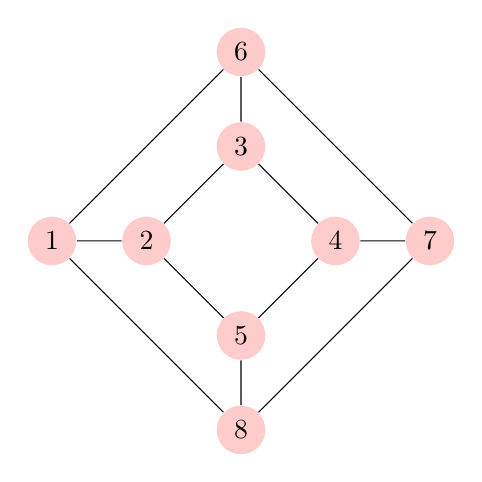
\begin{tikzpicture}
  [scale=.6,auto=left,every node/.style={circle,fill=red!20}]
  \node (n1) at (1,7) {1};
  \node (n2) at (3,7)  {2};
  \node (n4) at (7,7) {4};
  \node (n7) at (9,7)  {7};
  \node (n6) at (5,11)  {6};
   \node (n3) at (5,9) {3};
   \node (n5) at (5,5) {5};
   \node (n8)  at (5,3) {8};
  \foreach \from/\to in {n1/n2,n2/n3,n3/n4,n4/n5,n5/n2,n1/n6,
  n6/n7, n7/n8, n8/n1, n3/n6, n4/n7, n5/n8}
    \draw (\from) -- (\to);

\end{tikzpicture}
\caption{ Cube Graph }\label{5g1}
\end{center}
\end{figure}

Ajur thought about for a few seconds and he drew the Hamiltonian cycle of Figure \ref{5g1} in Figure \ref {5g2}. Krishnak told Ajur that his solution is not unique and there are more solutions!\footnote{Please find a Hamiltonian Cycle distinct from the one mentioned here}

\begin{figure}
\begin{center}
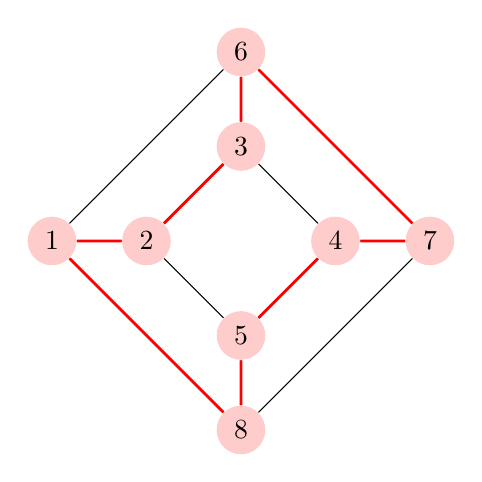
\begin{tikzpicture}
  [scale=.6,auto=left,every node/.style={circle,fill=red!20}]
  \node (n1) at (1,7) {1};
  \node (n2) at (3,7)  {2};
  \node (n4) at (7,7) {4};
  \node (n7) at (9,7)  {7};
  \node (n6) at (5,11)  {6};
   \node (n3) at (5,9) {3};
   \node (n5) at (5,5) {5};
   \node (n8)  at (5,3) {8};
  \foreach \from/\to in {n1/n2,n2/n3,n3/n4,n4/n5,n5/n2,n1/n6,
  n6/n7, n7/n8, n8/n1, n3/n6, n4/n7, n5/n8}
    \draw (\from) -- (\to);
\path[line width=0.35mm,red] (n1) edge (n2)
(n2) edge (n3)
(n3) edge (n6)
(n6) edge (n7)
(n7) edge (n4)
(n4) edge (n5)
(n5) edge (n8)
(n8) edge (n1);
\end{tikzpicture}
\caption{ Cube Graph with Hamiltonian  Cycle marked in thick edges}\label{5g2}
\end{center}
\end{figure}

Rishnak then told Ajur what led Hamilton to the statement of the Hamiltonian cycle problem. The mathematician Hamilton wanted a cycle to visit 
all the vertices of a Dodecahedron (another platonic solid, like cube) which has 20 vertices and 30 edges. 
Rishnak asked Ajur whether there is a Hamiltonian Cycle in this graph Figure \ref{5g3}. Rishnak added that this is a well known graph known as Petersen Graph.

\begin{figure}
\begin{center}
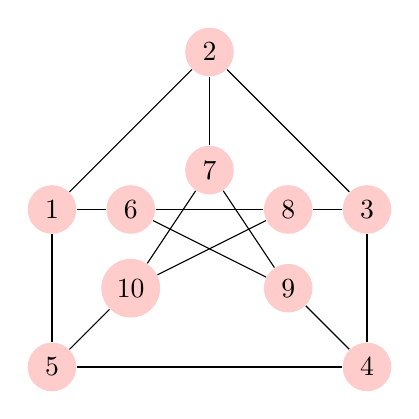
\begin{tikzpicture}
  [scale=.5,auto=left,every node/.style={circle,fill=red!20}]
  \node (n1) at (1,7) {1};
  \node (n2) at (5,11)  {2};
  \node (n3) at (9,7)  {3};
  \node (n4) at (9,3) {4};
  \node (n5) at (1,3) {5};
  \node (n6) at (3,7)  {6};
  \node (n7) at (5,8) {7};
  \node (n8)  at (7,7) {8};
  \node (n9) at (7,5) {9};
  \node (n10) at  (3,5) {10};
 
  \foreach \from/\to in {n1/n2,n2/n3,n3/n4,n4/n5,n5/n1,n1/n6,
  n2/n7, n3/n8, n4/n9, n5/n10, n6/n8, n8/n10, n10/n7,n7/n9,n9/n6}
    \draw (\from) -- (\to);

\end{tikzpicture}
\caption{ Petersen Graph with 10 vertices and 15 edges }\label{5g3}
\end{center}
\end{figure}
Ajur thought for a while and he was not able to construct a Hamiltonian cycle. He however, was able to find a 
Hamiltonian Path. So he drew the following Figure \ref{5g4}. Rishnak mentioned to Ajur that this Hamiltonian path is not unique and there are other Hamiltonian paths.\footnote{Find a Hamiltonian path distinct from the one shown here.}


\begin{figure}
\begin{center}
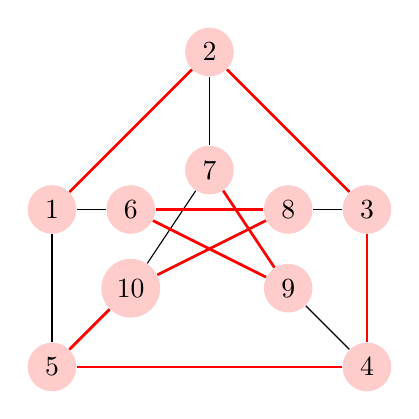
\begin{tikzpicture}
  [scale=.5,auto=left,every node/.style={circle,fill=red!20}]
  \node (n1) at (1,7) {1};
  \node (n2) at (5,11)  {2};
  \node (n3) at (9,7)  {3};
  \node (n4) at (9,3) {4};
  \node (n5) at (1,3) {5};
  \node (n6) at (3,7)  {6};
  \node (n7) at (5,8) {7};
  \node (n8)  at (7,7) {8};
  \node (n9) at (7,5) {9};
  \node (n10) at  (3,5) {10};
 
  \foreach \from/\to in {n1/n2,n2/n3,n3/n4,n4/n5,n5/n1,n1/n6,
  n2/n7, n3/n8, n4/n9, n5/n10, n6/n8, n8/n10, n10/n7,n7/n9,n9/n6}
    \draw (\from) -- (\to);
\path[line width=0.35mm,red]
(n1) edge (n2)
(n2) edge (n3)
(n3) edge (n4)
(n4) edge (n5)
(n5) edge (n10)
(n10) edge (n8)
(n8) edge (n6)
(n6) edge (n9)
(n9) edge (n7);

\end{tikzpicture}
\caption{ Petersen Graph with a Hamiltonian Path}\label{5g4}
\end{center}
\end{figure}
Rishnak assured Ajur that Petersen Graph does not have a Hamiltonian Cycle. Whether a graph has an Eulerian Cycle or not can easily be tested (the degree of every vertex has to be even), however, there is no easy way for test whether a given graph has a Hamiltonian cycle. 
Rishnak continued that there is a special class of graphs called bipartite graphs where every cycle is of even length. The vertex set can be partitioned into two sets $A$ and $B$, such that every edge in such a graph has one end vertex in $A$ and the other end vertex in $B$. Rishnak showed an example Figure \ref{5g5}. Ajur immediately said that all the cycles are of even lengths (4 and 6).\footnote{Every edge in the cycle must go from one partition to the other partition(they are the only possible edges)= hence the cycle length has to be even.} Rishnak asked Ajur what the two vertex partitions are (all the edges go from one partition to the other). After a little thought Ajur said one partition contains 1, 3, 5 and the other partition contains the vertices 2, 4 and 6. Ajur drew a graph (see Figure \ref{5g55}) to illustrate  what he meant. Ajur also mentioned that this graph has a Hamiltonian cycle. \footnote{Ajur exclaimed that every tree is a bipartite graph too, as a tree contains no cycles (or cycles of length 0 - we know that 0 is an even number!). Rishnak reminded Ajur that since tree does not have cycles and hence no Hamiltonian cycles.} 
Ajur wanted to show that he has understood the concept of bipartite graphs. So he drew a graph - see Figure \ref{5g6} that does not have a Hamiltonian cycle. Ajur explained why this graph does not have a Hamiltonian cycle. If there were a Hamiltonian cycle, the vertices in the cycle have to alternate between the two vertex partitions. But one vertex partition has two vertices and the other vertex partition has three vertices. Rishnak smiled and appreciated Ajur's logical thinking.

\begin{figure}
\begin{center}
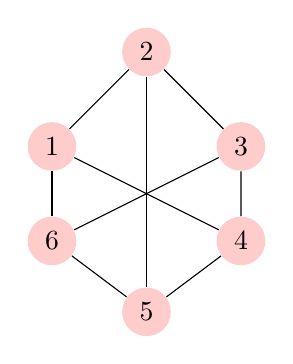
\begin{tikzpicture}
  [scale=.3,auto=left,every node/.style={circle,fill=red!20}]
  \node (n1) at (1,7) {1};
  \node (n2) at (5,11)  {2};
  \node (n3) at (9,7)  {3};
  \node (n4) at (9,3) {4};
  \node (n5) at (5,0)  {5};
  \node (n6) at (1,3) {6};
  
   \foreach \from/\to in {n1/n2,n2/n3,n3/n4,n4/n5,n5/n6,n1/n6,
  n2/n5, n6/n3,n1/n4}
    \draw (\from) -- (\to);
    \end{tikzpicture}
\caption{ A Bipartite Graph with 6 vertices and 9 edges}\label{5g5}
\end{center}
\end{figure}
\begin{figure}
\begin{center}
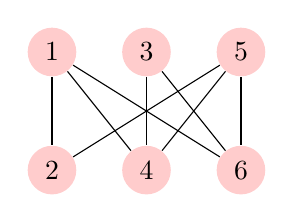
\begin{tikzpicture}
  [scale=.3,auto=left,every node/.style={circle,fill=red!20}]
  \node (n1) at (1,7) {1};
  \node (n3) at (5,7)  {3};
  \node (n5) at (9,7) {5};
  \node (n2) at (1,2)  {2};
  \node (n4) at (5,2) {4};
  \node (n6) at (9,2)  {6};
 
  
   \foreach \from/\to in {n1/n2,n1/n4,n1/n6,n3/n4,n3/n6,n5/n2,n5/n4,n5/n6}
    \draw (\from) -- (\to);
    \end{tikzpicture}
\caption{ Graph in \ref{5g5} drawn with vertex partition}\label{5g55}
\end{center}
\end{figure}
\begin{figure}
\begin{center}
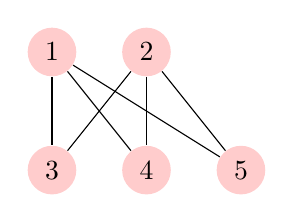
\begin{tikzpicture}
  [scale=.3,auto=left,every node/.style={circle,fill=red!20}]
  \node (n1) at (1,7) {1};
  \node (n2) at (5,7)  {2};
  \node (n3) at (1,2)  {3};
  \node (n4) at (5,2) {4};
  \node (n5) at (9,2)  {5};
 
  
   \foreach \from/\to in {n1/n3,n1/n4,n1/n5,n2/n3,n2/n4,n2/n5}
    \draw (\from) -- (\to);
    \end{tikzpicture}
\caption{ A Bipartite Graph with 5 vertices and 6 edges}\label{5g6}
\end{center}
\end{figure}

Rishnak then told Ajur about a problem he had heard in the radio program called Car Talk broadcast over the public radio. Here is a simplified version of the puzzle in the show.\footnote{ attributed to Bruce Robinson, a professor of civil and environmental engineering at the University of Tennessee} There are 9 jealous people who live in the squares of a three-by-three grid (see Figure \ref{5g7}. The squares are numbered, starting on the upper left-hand corner, 1 through 9. (going across one row at time or one column at a time or how?) Each person is jealous of his adjacent neighbor. Not his diagonal neighbor, but the person up or down or left or right of him. Each aspires to move into the apartment of his adjacent neighbor.
The question is very simple: What is the fewest number of total moves that can accomplish this?
\begin{figure}
\begin{center}
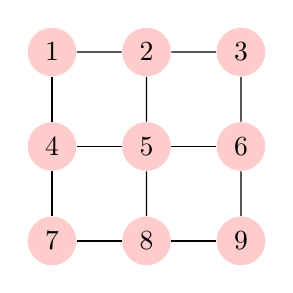
\begin{tikzpicture}
  [scale=.3,auto=left,every node/.style={circle,fill=red!20}]
  \node (n1) at (1,11) {1};
  \node (n2) at (5,11)  {2};
  \node (n3) at (9,11) {3};
  \node (n4) at (1,7)  {4};
  \node (n5) at (5,7) {5};
  \node (n6) at (9,7)  {6};
  \node (n7) at (1,3)  {7};
  \node (n8) at (5,3) {8};
  \node (n9) at (9,3)  {9};
  
  
   \foreach \from/\to in {n1/n2,n1/n4,n2/n3,n2/n5,n3/n6,n4/n5,n4/n7,n5/n6,n5/n8,n6/n9,n7/n8,
   n8/n9}
    \draw (\from) -- (\to);
    \end{tikzpicture}
\caption{ A three by three grid with nine apartments. Apartments are modeled as vertices and an edge denotes adjacency relation between apartments (up, down, two sides - not all apartments have all of the adjacent apartments} \label{5g7}
\end{center}
\end{figure}

Ajur immediately figured  this is a bipratite graph and the partitions are not of equal size. Hence immediately he responded that this is not possible. Rishnak asked Ajur to write it so that his argument is tight. Ajur promised that he will do it by next day. This graph has a Hamiltonian path but not a Hamiltonian cycle. Ajur said that instead of three by three grid of apartments, if we had a four by three grid (or three by four grid) of apartments, it is easy for all of them to transfer to the adjacent apartments. Such a graph has a Hamiltonian Cycle.

Euler proposed a Knight's tour problem on a chessboard. A chessboard is an eight by eight square. Place a knight in any square. From that square, knight has to move\footnote{knight moves either two squares vertically up/down and one square horizontally left or right or one square vertically up or down and two squares horizontally left or right} visiting all squares once and only once. You can think of this as finding a Hamiltonian path in a 64 vertex graph with two vertices being adjacent if there is a knight move from one vertex to the other. There is no easy method of finding a knight's tour other than exhaustive search.\footnote{Usual method of exhaustive search is through backtracking - a systematic method of exploring all possibilities} Here is a solution Table \ref{5t1} for a five by five chess board with the knight's tour starting from bottom left.
\begin{table}
\centering
\begin{tabular}{|c |c |c| c| c|} 
 \hline
3&10&21&16& 5\\
\hline
20&15& 4&11&22\\
\hline
 9& 2&23& 6&17\\
 \hline
14&19& 8&25&12\\
\hline
 1&24&13&18& 7\\
 \hline
\end{tabular}
\caption{Knight's Tour on five by five chess board starts at the bottom left}
\label{5t1}
\end{table}
Rishnak asked Ajur to find the message is encoded here in this table \ref{5t2}.
\begin{table}
\centering
\begin{tabular}{c c c c cc}
i& t& t& t& b& l\\
r& h &d &e& u& s\\
h& a& y& e& d& o\\
a& o& e& p& r& n\\
s& n& f& o& l& l\\
f& v& d &i& e& u\\
\end{tabular}
\caption{What is the Message is encoded here}
\label{5t2}
\end{table}
Rishnak added that there are poems from different cultures (including India and China) based on Knight's tour. Ajur was intrigued and resolved to read and understand the poems. Rishnak added that one needs to verify that a knight's tour is impossible for a three by three chessboard or a four by four chessboard and warned that checking whether a knight's tour is impossible also takes a long time.

There are many methods to check whether a given graph has a Hamiltonian cycle. Unfortunately these conditions are \textbf{not} exhaustive. Rishnak taught Ajur a simple test to know whether a graph has a Hamiltonian cycle.

Rishnak stated the well known theorem that if the degree of every vertex in a graph with $n$ vertices is $\ge~\frac{n}{2}$, then the graph has a Hamiltonian cycle. Rishnak added that one can prove this theorem by Induction.\footnote{Proof by Induction is a powerful method for proving  statements.  First you prove a base case (in our case here Graph with three vertices). Then assume it is true for all $n~ \le ~k$ vertices and prove for $n~=~k+1$ vertices.} The base case with three vertices meeting the condition is a three vertex graph in which every vertex is connected to every other vertex - That is the only graph that satisfies the condition that the degree of every vertex is $\ge~\frac{3}{2}$. That graph has a Hamiltonian cycle. Assume that the hypothesis (a graph with $k$ vertices with degree of every vertex is $\ge~\frac{k}{2}$ has a Hamiltonian cycle) is true for graphs with vertices $\le~ k$ vertices. Let that Hamiltonian cycle be $v_i,v_{i+1},\cdots v_i$. Now consider a graph with $k+1$ vertices. The new vertex $v_{k+1}$ has to have a degree at least $\frac{k+1}{2}$.  The new vertex has to be adjacent to at least two adjacent vertices in that Hamiltonian cycle. For if it were not the degree of the new vertex will be $\le~\frac{k}{2}$. Since the new vertex is adjacent to two adjacent vertices (call them $v_l$ and $v_{l+1}$) in the Hamiltonian cycle of the graph with $k$ vertices. Now you can create a new Hamiltonian cycle in the $k+1$ vertex graph by $v_i,v_{i+1},\cdots,v_l,v_{k+1},v_{l+1},\cdots,v_i$. 

Ajur was able to follow along and loved the proof by Induction and the clever arguments used in the proof. But Jura who was patiently waiting was beginning to get restless so Ajur called it a day.

\chapter{Graph Isomorphism, Subgraph Isomorphism}

Rishnak was eagerly looking for Ajur because he wanted to share with him a new concepts and found Ajur and Jura walking along the bank of a (presumably haunted) pond in the cemetery. Rishnak started this session with a small variant on what they had been discussing. A graph whose vertices are labeled is called a labeled graph and one without labels for vertices is called an unlabeled graph. Two labeled graphs are equivalent if they are identical. The labeled graphs in Figures \ref{8g1} and \ref{8g11} are equivalent. The graph in Figure \ref{8g2} is not equivalent to the graph in Figures \ref{8g1} or \ref{8g11} or  \ref{8g2} as there is no edge between vertices 4 and 5.
\begin{figure}
\begin{center}
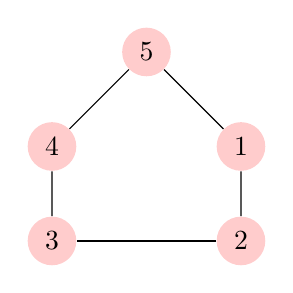
\begin{tikzpicture}
  [scale=.6,auto=left,every node/.style={circle,fill=red!20}]
  \node (n1) at (5,5) {1};
  \node (n4) at (1,5)  {4};
  \node (n3) at  (1,3) {3};
  \node (n2) at (5,3)  {2};
  \node (n5) at (3,7)  {5};

  \foreach \from/\to in {n1/n2,n2/n3,n3/n4,n4/n5,n1/n5}
    \draw (\from) -- (\to);

\end{tikzpicture}
\caption{Labeled Graph}\label{8g1}
\end{center}

\end{figure}
\begin{figure}
\begin{center}
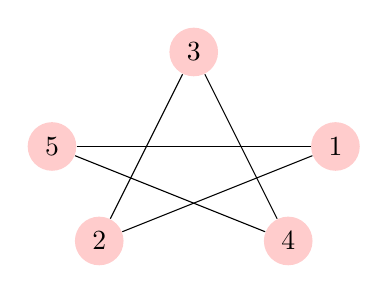
\begin{tikzpicture}
  [scale=.6,auto=left,every node/.style={circle,fill=red!20}]
   \node (n1) at (6,5) {1};
  \node (n5) at (0,5)  {5};
  \node (n2) at  (1,3) {2};
  \node (n4) at (5,3)  {4};
  \node (n3) at (3,7)  {3};

  \foreach \from/\to in {n1/n2,n2/n3,n3/n4,n4/n5,n5/n1}
    \draw (\from) -- (\to);

\end{tikzpicture}
\caption{ Another labeled graph with five vertices equivalent to Figure \ref{8g1}}\label{8g11}
\end{center}
\end{figure}

\begin{figure}
\begin{center}
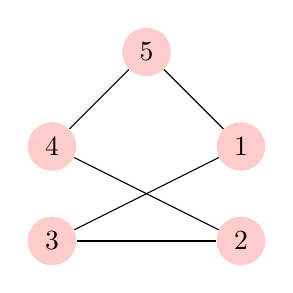
\begin{tikzpicture}
  [scale=.6,auto=left,every node/.style={circle,fill=red!20}]
   \node (n1) at (5,5) {1};
  \node (n4) at (1,5)  {4};
  \node (n3) at  (1,3) {3};
  \node (n2) at (5,3)  {2};
  \node (n5) at (3,7)  {5};


  \foreach \from/\to in {n1/n3,n2/n4,n3/n2,n1/n5,n5/n4}
    \draw (\from) -- (\to);

\end{tikzpicture}
\caption{ Another labeled graph with five vertices which is not equivalent to Graphs \ref{8g1} and \ref{8g11} as the edge labels are distinct from either of the two graphs}\label{8g2}
\end{center}
\end{figure}

Rishnak continued rhetorically: ``when are two graphs the same"? Two graphs are isomorphic (\emph{structurally the same}), if they are equivalent under a vertex relabeling. For example, if in the graph of Figure \ref{8g2} vertex 2 is relabeled as 3 and vertex 3 is relabeled as 2, then two graphs in Figures \ref{8g2} and \ref{8g1} are equivalent. If a graph, $G$, is equivalent to a graph $H$ and $H$ is equivalent to another graph $P$, then $G$ is equivalent to graph $P$\footnote{In other words, the relation of being equivalent graphs is transitive.}. To test whether two graphs are isomorphic are not is a hard problem\footnote{Not as hard as finding a Hamiltonian Cycle in a graph} .

If two graphs are isomorphic, they should have the same number of vertices, the same number of edges, the same degree sequences, the same length of the longest cycle, and the same length of the shortest cycle.  These properties of graphs are called graph invariants. By no mean are these invariants are exhaustive. We do not know of a single easily computable invariant that can be used to test whether or not two given graphs are isomorphic. 

Rishnak asked Ajur, to provide two graphs which have the same number of vertices and same number of edges but they are not isomorphic. Ajur thought a bit and he was able to produce the following two graphs which have 6 vertices and 9 edges. Ajur added that one graph is bipartite (all cycles are of even length) \ref{8g3} and the other one is not bipartite (it has cycle of length 3) \ref{8g4} and hence these two graphs are not isomorphic.

\begin{figure}

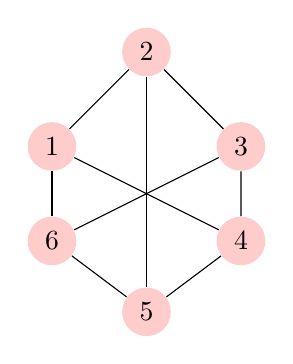
\begin{tikzpicture}
  [scale=.3,auto=left,every node/.style={circle,fill=red!20}]
  \node (n1) at (1,7) {1};
  \node (n2) at (5,11)  {2};
  \node (n3) at (9,7)  {3};
  \node (n4) at (9,3) {4};
  \node (n5) at (5,0)  {5};
  \node (n6) at (1,3) {6};
  
   \foreach \from/\to in {n1/n2,n2/n3,n3/n4,n4/n5,n5/n6,n1/n6,
  n2/n5, n6/n3,n1/n4}
    \draw (\from) -- (\to);
    \end{tikzpicture}
\caption{ A Bipartite Graph with 6 vertices and 9 edges same as Graph in \ref{5g5}}\label{8g3}

\end{figure}

\begin{figure}

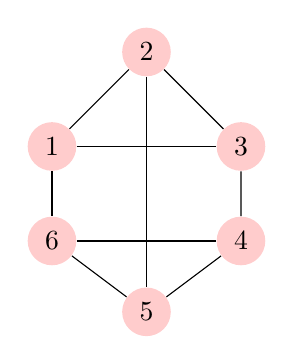
\begin{tikzpicture}
  [scale=.3,auto=left,every node/.style={circle,fill=red!20}]
  \node (n1) at (1,7) {1};
  \node (n2) at (5,11)  {2};
  \node (n3) at (9,7)  {3};
  \node (n4) at (9,3) {4};
  \node (n5) at (5,0)  {5};
  \node (n6) at (1,3) {6};
  
   \foreach \from/\to in {n1/n2,n2/n3,n3/n4,n4/n5,n5/n6,n1/n6,
  n2/n5, n6/n4,n1/n3}
    \draw (\from) -- (\to);
    \end{tikzpicture}
\caption{ A nonbipartite Graph with 6 vertices and 9 edges}\label{8g4}

\end{figure}

Ajur thought for a while and said that partial solutions to the isomorphism problem would be very useful when you want to test whether a given graph is in a collection of graphs, a problem that comes up in chemistry. Rishnak was pleased to notice that Ajur was thinking about practical applications of graph theory. 

Ajur wanted to know if there is an easier method for testing isomorphism between rooted trees. Rishnak smiled and said there is a faster method for rooted trees. First, Rishnak explained a certain canonical representation for a labeled tree, called a Pr\"ufer code. The construction is iterative, and the Pr\"ufer code of a labeled tree with $n$ vertices is a code of length $n-2$. First, we recall that a leaf of a tree is a vertex that is connected to only one other vertex.

\begin{enumerate}
\item let Pr{\"u}fer code be an empty set,

\item Start with a leaf vertex of smallest label, say v. Find the vertex connecting it to the rest of tree say w.  Remove v from the tree and add w to the Pr{\"u}fer Code
 
\item Repeat the previous step until we are left with two vertices.
\end{enumerate}

We implement this procedure for the following tree, in Example \ref{8g5}. The smallest leaf vertex is 4. Its adjacent vertex is labeled 2. So 2 is added to the Pr{\"u}fer code and vertex 4 is removed. Next smallest vertex is 5 and its adjacent vertex is 2. Hence 2 is added to the Pr{\"u}fer code and vertex labeled 5 is removed. Now 2 is the smallest leaf vertex and its adjacent vertex is 1 and  1 is added to Pr{\"u}fer code and vertex 2 is removed. Currently Pr{\"u}fer code is \textbf{221}. Now 1 is the smallest labeled vertex and its adjacent vertex is 3 and vertex 1 is removed. Hence 3 is added to Pr{\"u}fer code which becomes \textbf{2213}. The next smallest leaf vertex is 6 and its adjacent vertex is 3. 3 is added to Pr{\"u}fer code. There are only two vertices left and we are done. The Pr{\"u}fer code for tree in Example \ref{8g5} is \textbf{22133}. From this Pr{\"u}fer code, one can conclude that there are 7 vertices in the tree (as the Pr{\"u}fer code is of length $n-2$ for a tree with $n$ vertices). Further, we can also conclude that vertices labeled 4,5,6 and 7 are leaf vertices as they do not appear in the given Pr{\'u}fer code. 
\begin{figure}
\begin{center}

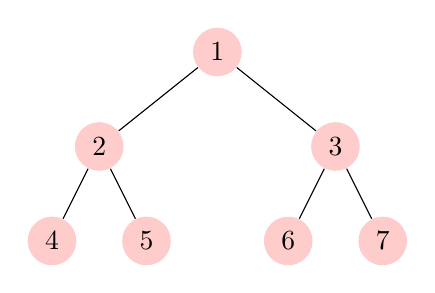
\begin{tikzpicture}
  [scale=.6,auto=left,every node/.style={circle,fill=red!20}]
  \node (n1) at (5.5,7) {1};
  \node (n2) at (3,5)  {2};
  \node (n3) at (8,5)  {3};
  \node (n4) at (2,3) {4};
  \node (n5) at (4,3)  {5};
  \node (n6) at (7,3)  {6};
  \node (n7) at (9,3)  {7};

  \foreach \from/\to in {n1/n2,n1/n3,n2/n4,n2/n5,n3/n6,n3/n7}
    \draw (\from) -- (\to);

\end{tikzpicture}

\caption{Tree with 7 vertices and four leaf vertices }\label{8g5}
\end{center}
\end{figure}

Ajur then wanted to know if one could have a code for unlabeled trees. Rishnak replied with a resounding yes and explained the basic steps for a rooted tree. For any tree, one needs to choose an appropriate root vertex \footnote{Center of a tree is chosen as the root vertex}  %\textbf{Raju: be careful, not every tree has a center which is a vertex!}} 
\begin{enumerate}
    \item  Label the leaf vertices as 01.
    \item Let $x$ be a non-leaf vertex. If all the children of $x$, sort these labels in alphabetical order. \footnote{0 comes before 1} The label of vertex $x$ is 0 followed by concatenation of the (sorted) labels of the children followed by 1.
    \item Stop after you label the root vertex.
\end{enumerate}

For example for the tree in \ref{8g5} leaf vertices 4,5,6,7 are all labeled \textbf{01}. Vertex 2 is labeled \textbf{001011} and vertex 3 has a similar label \textbf{001011}. Finally root vertex has the label \textbf{00101100101111}. This \textbf{00101100101111} becomes the code for the tree.

Rishnak continued that closely related to Graph Isomorphism is a problem that has plenty of uses in real life - and not just in the ghoulish realm. Ajur chuckled at the bad joke but politely retrained from interrupting. Rishank continued with the statement of the next problem.  Instead of asking whether two graphs are structurally similar, given two graphs $G$ and $H$, the subgraph isomorphism problem asks if there is a subgraph of $G$ that is isomorphic to H. Ajur responded immediately saying this approach can be used to test if a graph $G$ with $n$ vertices has a Hamiltonian cycle by choosing $H$ to be a cycle of length $n$ and asking whether there is a subgraph of $G$ isomorphic to $H$. Rishnak nodded in agreement and said that is the reason the subgraph Isomorphism problem is hard. On the other hand, if both $G$ and $H$ are labeled graphs, there are heuristics to test whether $H$ occurs in $G$ as a subgraph. This type of labeled subgraph isomorphism problem has many applications in medical imaging and chemical structure identifications.

\textbf{Question for the sixth day:} Rishnak asked Ajur to draw a tree whose Pr{\"u}fer code is 232.

\textbf{Answer} Ajur realized this is a tree with five vertices and he drew the following tree Figure \ref{6q1}.
\begin{figure}
\begin{center}

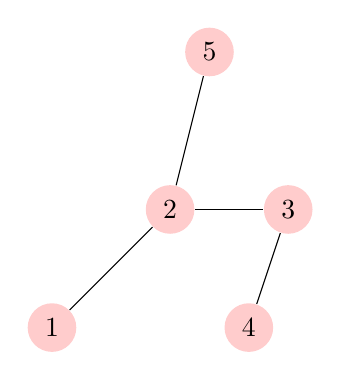
\begin{tikzpicture}
  [scale=.5,auto=left,every node/.style={circle,fill=red!20}]
  \node (n1) at (0,0) {1};
  \node (n2) at (3,3)  {2};
  \node (n3) at (6,3)  {3};
  \node (n4) at (5,0) {4};
  \node (n5) at (4,7)  {5};
 

  \foreach \from/\to in {n1/n2,n4/n3,n2/n3,n2/n5}
    \draw (\from) -- (\to);

\end{tikzpicture}

\caption{Tree with 5 vertices}\label{6q1}
\end{center}
\end{figure}

Rishnak was happy with Ajur's answer and Ajur was eager to go with Jura.
\chapter{Planar Graphs}
Ajur was so enamored by Hamiltonian cycles, he was eager to meet Rishnak and learn more about them, but Rishnak wanted to introduce a different concept: drawing graphs.

Ajur said, ``I already know how to draw graphs.''

Rishnak said, ``Wait, Ajur, there's much more to it. Listen. A planar drawing of a graph is one in which no edges cross each other (except at their endpoint vertices). By definition, a \textit{planar graph} \index{planar graph} is a graph for which there exists at least one planar drawing. And if a graph does not have any possible planar drawings, we call it a \textit{non-planar graph}.''

\begin{figure}
\begin{center}
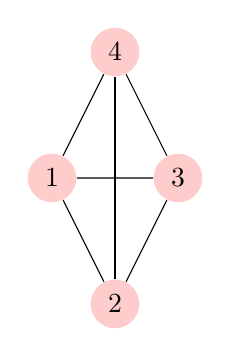
\begin{tikzpicture}
  [scale=.4,auto=left,every node/.style={circle,fill=red!20}]
  \node (n1) at (1,7) {1};
  \node (n2) at (3,3)  {2};
  \node (n3) at (5,7)  {3};
  \node (n4) at (3,11)  {4};

  \foreach \from/\to in {n1/n2,n2/n3,n2/n4,n1/n4,n3/n4,n1/n3} 
  \draw (\from) -- (\to);

\end{tikzpicture}
\caption{A drawing of complete graph~$K_4$ in which two edges cross}\label{9g1}
\end{center}
\end{figure}

In a dazzling flash of light, Rishnak waved his hands and two graphs appeared [Figure~\ref{9g1}] [Figure~\ref{9g2}]. He said, ``For example, here are two drawings of complete graph~$K_4$, the~4 in this case meaning we have four vertices. Notice that the second graph [Figure~\ref{9g2}] has no edges that cross, so we call~$K_4$ a planar graph. In other words, it displays nicely on a two-dimensional plane.''

\begin{figure}
\begin{center}
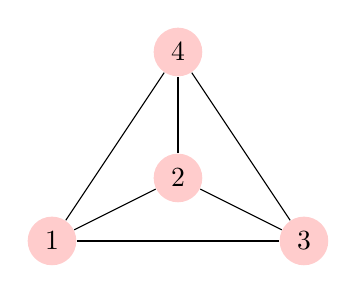
\begin{tikzpicture}
  [scale=.4,auto=left,every node/.style={circle,fill=red!20}]
  \node (n1) at (-1,7) {1};
  \node (n2) at (3,9)  {2};
  \node (n3) at (7,7)  {3};
  \node (n4) at (3,13)  {4};

  \foreach \from/\to in {n1/n2,n2/n3,n2/n4,n1/n4,n3/n4,n1/n3}
    \draw (\from) -- (\to);

\end{tikzpicture}
\caption{A planar drawing of~$K_4$ in which no edges cross}\label{9g2}
\end{center}
\end{figure}

\begin{figure}
\begin{center}
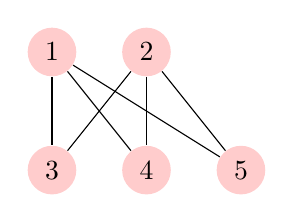
\begin{tikzpicture}
  [scale=.3,auto=left,every node/.style={circle,fill=red!20}]
  \node (n1) at (1,7) {1};
  \node (n2) at (5,7)  {2};
  \node (n3) at (1,2)  {3};
  \node (n4) at (5,2) {4};
  \node (n5) at (9,2)  {5};

   \foreach \from/\to in {n1/n3,n1/n4,n1/n5,n2/n3,n2/n4,n2/n5}
    \draw (\from) -- (\to);
    \end{tikzpicture}
\caption{Bipartite graph~$K_{2,3}$ with five vertices and six edges in which four edges cross}\label{9g3}
\end{center}
\end{figure}

Rishnak asked, ``So, Ajur, can you draw this graph''---he waved his hands and a new graph appeared [Figure~\ref{9g3}]---``as a planar graph, that is, with no edges that cross?''

Ajur studied the graph and found the task to be a bit challenging. Then, he thought of moving vertex~2 down below vertex~4, thinking that would help separate the crossed edges. He picked up a stick and drew a graph in the dirt [Figure~\ref{9g4}], smiling as he realized he had solved the problem.

\begin{figure}
\begin{center}
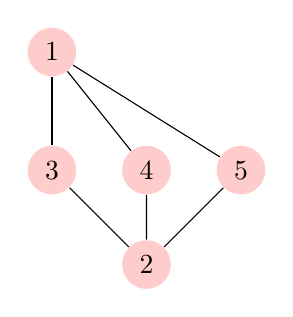
\begin{tikzpicture}
  [scale=.3,auto=left,every node/.style={circle,fill=red!20}]
  \node (n1) at (1,7) {1};
  \node (n2) at (5,-2)  {2};
  \node (n3) at (1,2)  {3};
  \node (n4) at (5,2) {4};
  \node (n5) at (9,2)  {5};

   \foreach \from/\to in {n1/n3,n1/n4,n1/n5,n2/n3,n2/n4,n2/n5}
    \draw (\from) -- (\to);
    \end{tikzpicture}
\caption{A planar drawing of bipartite graph~$K_{2,3}$ with five vertices and six edges}\label{9g4}
\end{center}
\end{figure}

Impressed, Rishnak waved his hands and another new graph appeared [Figure~\ref{9g5}]. He asked Ajur whether this new graph had a planar representation or not.

Ajur worked at this problem for some time, struggling to find a planar drawing.

At length, he said, ``I can only come up with this graph''---he pointed to the graph he had drawn [Figure~\ref{9g6}]---``but there's one edge crossing I can't get rid of.''

\begin{figure}
\begin{center}
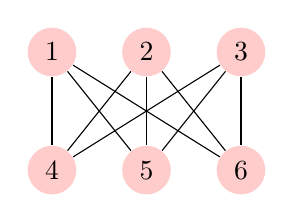
\begin{tikzpicture}
  [scale=.3,auto=left,every node/.style={circle,fill=red!20}]
  \node (n1) at (1,7) {1};
  \node (n2) at (5,7)  {2};
  \node (n3) at (9,7) {3};
  \node (n4) at (1,2)  {4};
  \node (n5) at (5,2) {5};
  \node (n6) at (9,2)  {6};

   \foreach \from/\to in {n1/n6,n1/n4,n1/n5,n2/n6,n2/n4,n2/n5,n3/n4,n3/n5,n3/n6}
    \draw (\from) -- (\to);
    \end{tikzpicture}
\caption{Bipartite graph~$K_{3,3}$ with six vertices and nine edges in which seven of the edges cross}\label{9g5}
\end{center}
\end{figure}

\begin{figure}
\begin{center}
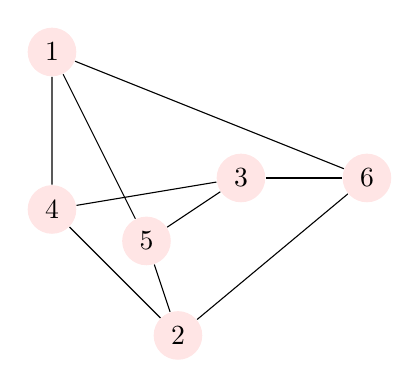
\begin{tikzpicture}
  [scale=.4,auto=left,every node/.style={circle,fill=red!10}]
  \node (n1) at (1,7) {1};
  \node (n2) at (5,-2)  {2};
  \node (n3) at (7,3) {3};
  \node (n4) at (1,2)  {4};
  \node (n5) at (4,1) {5};
  \node (n6) at (11,3)  {6};

   \foreach \from/\to in {n1/n6,n1/n4,n1/n5,n2/n6,n2/n4,n2/n5,n3/n4,n3/n5,n3/n6}
    \draw (\from) -- (\to);
    \end{tikzpicture}
\caption{A drawing of bipartite graph~$K_{3,3}$ in which just two edges edges cross}\label{9g6}
\end{center}
\end{figure}

Rishnak told Ajur that bipartite graph~$K_{3,3}$ does not have a planar representation. He said, ``There is a well-known related puzzle credited to Sam Loyd, an American recreational mathematician and puzzler. Let's say there are three houses, which we can represent as vertices~1, 2, and~3 of~$K_{3,3}$, drawn on paper. Below them are three vertices~4, 5, and~6 representing gas, water, and electricity suppliers. The aim of the puzzle is to draw lines to get each utility into every house, but---''

Ajur chimed in, ``But without crossing any of the lines.'' Ajur laughed at the puzzle, thinking that he should read up on Loyd's puzzle books the next time he visited his local library.

Rishnak cleared his throat, not entirely happy that Ajur cut him off. He said, ``If two graphs~$G$ and~$H$ are isomorphic and if~$G$ is planar, can you say that~$H$ is also planar?''

Ajur said, ``Yes, if~$H$ is isomorphic to~$G$, then each vertex of~$H$ corresponds to some vertex of~$G$. By just relabeling the vertices of~$G$ in its planar drawing, we can obtain a planar drawing of~$H$.''

Rishnak nodded and asked, ``What can we say about trees?''

Ajur thought for a moment, then said, ``That's easy. All trees have a planar representation\footnote{Ajur liked monkeys and monkeys liked trees. It follows by transitivity that Ajur liked trees.} because there are no cycles.''

Rishnak said, ``Right, trees are indeed easy to embed in a plane as there are no cycles. There are some interesting space-filling planar representations of trees, for example this one''---he waved his hands and an intricate planar drawing appeared in front of Ajur [Figure~\ref{9g7}]. \index{space filling tree}

Ajur marveled at the drawing.

Rishnak continued, ``One way to get a planar drawing of a graph is to first embed the longest cycle in a plane, then try to place the rest of the vertices so that no edges cross one another. The longest cycle will divide the plane into two regions, an inner region (inside the cycle) and an outer region (outside the cycle).''

Ajur said, ``So the edges have to go either inside or outside the longest cycle.''

Rishnak said, ``Precisely. By trying out various possibilities, backtracking as necessary, you can eventually get a planar representation of a graph---if one exists. Of course, this process is easier said than done.''

Ajur asked, ``Is there any easier way?''

Rishnak said, ``There is in fact an efficient method of placing the edges, without any backtracking, but the details are rather complicated.'' %% maybe a footnote here describing how or where to look to read more?

\begin{figure}
\begin{center}    

 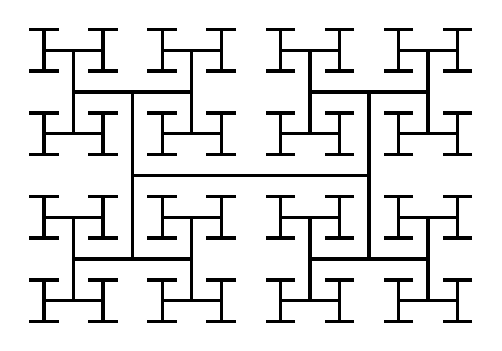
\begin{tikzpicture}[decoration=H-tree, very thick]
    \draw decorate { decorate { decorate { decorate { decorate { decorate { (0,0) -- (3,0) }}}}}};
  \end{tikzpicture}
  \caption{A planar drawing of a tree, which is self-similar}\label{9g7}
  \end{center}
\end{figure}

After a few minutes of silence in which Ajur thought about how this might work, Rishnak said, ``Remember Euler?''

Ajur nodded.

Rishnak waved his hands and a new graph appeared [Figure~\ref{fig:tetra}]. He said, ``Euler discovered a remarkable relationship between planar graphs and three-dimensional solids.  This planar graph represents a tetrahedron---a pyramid.''

Ajur asked, ``How is that a pyramid? It's two-dimensional.''

Rishnak chuckled and said, ``If you imagine stretching vertex~$a3$ out toward you, you end up with a three-dimensional solid with four sides, hence the name tetrahedron.''

Ajur studied the graph and said, ``Oh, I see now.''

Rishnak continued, ``Think of each region in a planar representation as the \textit{face} of such a three-dimensional solid. Then Euler's formula relating the number of edges~$e$, the number of vertices~$n$, and the number of faces~$f$ of a planar graph is simply this.''
\index{Euler's formula}
Rishnak waved his hands and Euler's equation appeared as follows:
\begin{equation}
\label{eqn:euler}
  f-e+n=2
\end{equation}

\begin{figure}
\begin{center}
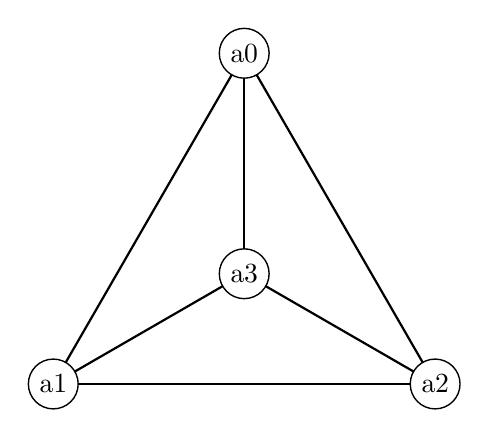
\begin{tikzpicture}
[scale=0.7]
        \grTetrahedral
    \end{tikzpicture}
\caption{Planar graph representing a tetrahedron}
\label{fig:tetra}
\end{center}
\end{figure}

Rishnak said, ``Let me explain this a bit. Each region corresponds to a cycle in the graph that surrounds that region. It also defines the external region, which is sometimes also called the infinite region. We know there are~$n-1$ edges in a tree, so if we can find that tree in the given graph, then the rest of the~$e-(n-1)$ edges will form part of a cycle. This gets tricky and we will have to explore this at some point in the future.\footnote{Rishnak and Ajur end up discussing this in Chapter~12 when they talk about spanning trees in a connected graph and how to choose one.}
%\textbf{You implicitly pick a spanning tree, which you have not yet discussed! Consider saying: it turns out, as we'll learn in Chapter ***, that there exists a ``maximal tree" of any graph.} 
Each of these cycles correspond to an internal region---in other words, an internal face---and one external face. From this, Euler's equation (\ref{eqn:euler}) follows.''

As Rishnak spoke, he drew the following equations in the air:
\begin{eqnarray}
    \label{eqn:cycles}
    \text{internal faces}&=&e-(n-1)\nonumber\\
    \text{external faces}&=&1 \nonumber \\
    \text{total faces}&=& \text{internal faces}~+~\text{external faces} \nonumber \\
    &=&e-n+2
\end{eqnarray}

Ajur studied the equations and understood, at least for a tetrahedron. He said, ``Okay, I've constructed Platonic solids with Zometool\footnote{Zometool is a commercial construction kit for making general polyhedra.}. Does this equation work for all of these?''

Rishnak smiled and said, ``Ah yes, the Platonic solids, named after Plato, the ancient Greek philosopher. And yes, Euler's equation applies to the five Platonic solids. In other words, the graph theory behind Euler's formula can be used to relate vertices, edges, and faces of the Platonic solids.''

Rishnak waved his hands and next to the graph corresponding to the tetrahedron [Figure~\ref{fig:tetra}], four more graphs appeared [Figure~\ref{fig:cube}] [Figure~\ref{fig:octa}] [Figure~\ref{fig:dod}] [Figure~\ref{fig:ico}]. He said, ``Ajur, can you write down the number of vertices~$n$, the number of edges~$e$, and the number of faces~$f$ for each of these?''

Ajur looked at each graph in turn, then systematically wrote the values in the dirt to create his table [Table~\ref{tab:platonic}].

Rishnak smiled and said, ``Good. All Platonic solids have a planar representation, as you can see in these graphs. The reason this works is that every solid fits within a sphere in such a way that no point or vertex passes through what would be the North pole. From this, one may stereographically project the graph onto the plane.''

\vspace{0.2in}
\begin{table}[ht]
    \centering
    \begin{tabular}{||c|c|c|c||}
    \hline
    Solid & n & e& f \\ [0.5ex] 
 \hline\hline
 Tetrahedron& 4 & 6 & 4 \\ 
 \hline
 Cube & 8 & 12 & 6 \\
 \hline
 Octohedron & 6 & 12& 8 \\
 \hline
 Dodecahedron & 20 & 30 & 12 \\
 \hline
 Icosahedron & 12 & 30 & 20 \\ [1ex] 
 \hline
 \end{tabular}
    \caption{Parameters of Euler's equation for the Platonic solids}
    \label{tab:platonic}
\end{table}

\begin{figure}
\begin{center}
    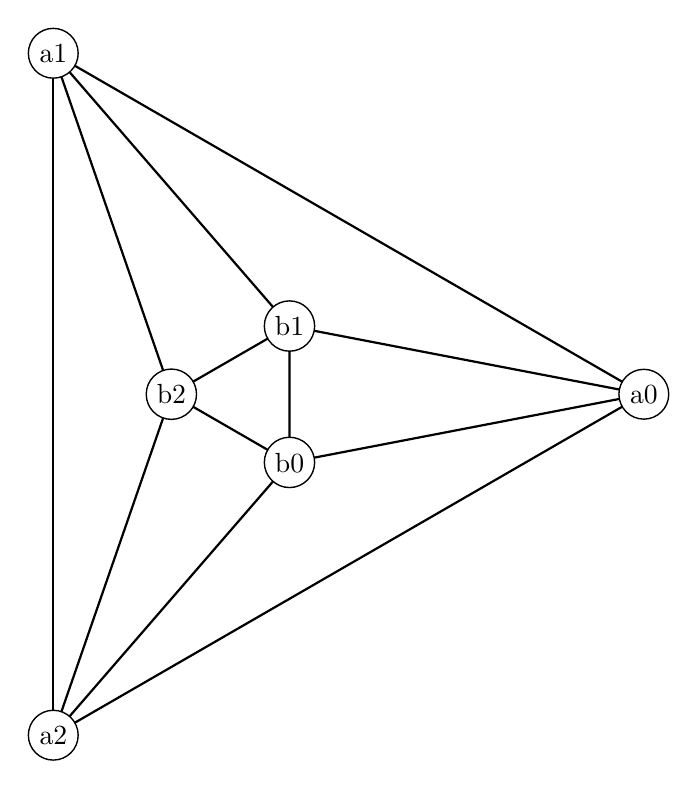
\begin{tikzpicture}

        \grOctahedral[RA=5,RB=1]
    \end{tikzpicture}
\caption{Planar graph representing a octahedron}\label{fig:octa}
\end{center}
\end{figure}
\begin{figure}
\begin{center}
    \begin{tikzpicture}

        \grCubicalGraph
    \end{tikzpicture}
\caption{Planar graph representing a cube}\label{fig:cube}
\end{center}
\end{figure}
\begin{figure}
\begin{center}
    \begin{tikzpicture}
    [scale=0.8]

        \grDodecahedral[form=2] 
    \end{tikzpicture}
    \caption{Planar graph representing a dodecahedron}\label{fig:dod}
\end{center}
\end{figure}
\begin{figure}
\begin{center}
    \begin{tikzpicture}

        \grIcosahedral[form=2,RA=8]
    \end{tikzpicture}
\caption{Planar graph representing a icosahedron}\label{fig:ico}
\end{center}
\end{figure}

Rishnak said, ``Notice that each edge appears in exactly two faces. If each face is a triangle---therefore a cycle of length~3---the graph is called a \textit{maximal planar graph}. From this, we can deduce~$e=\frac{3f}{2}$, or~$f=\frac{2e}{3}$. Substituting this for~$f$ in Euler's equation (\ref{eqn:euler})''---Rishnak waved his hands and equations floated in the air in front of Ajur---``we can solve for~$e$.'' \index{maximal planara graph}

\begin{eqnarray}
  \label{eqn:maxplanar}  
    \frac{2e}{3}&=&e-n+2\nonumber\\
    -\frac{e}{3} &=&-n+2\nonumber \\
    \frac{e}{3}&=&n-2 \nonumber \\
    e&=& 3n - 6
\end{eqnarray}

Rishnak paused after showing this equation (\ref{eqn:maxplanar}), giving Ajur time to think about it, then said, ``By using this equation, we can show that complete graph~$K_5$''---he flashed his hands and a new graph appeared [Figure~\ref{9g10}]---``is non-planar. This graph has five vertices and 10 edges, so~$n=5$ and~$e=10$. But from the equation, if it were planar, then the number of edges would have to be at most~$9$.''

Ajur raised his eyebrows and said, ``Aha, I see how that works. Nice!''

Rishnak asked Ajur, ``Can you use Euler's equation to show that complete bipartite graph~$K_{3,3}$ [Figure~\ref{9g5}] with its six vertices is non-planar?''

Ajur was alert and knew that a bipartite graph only has even cycle lengths. He said, ``To have the maximum number of edges, each face has to have a cycle length of~4. Therefore,~$2e=4f$ or~$f=\frac{e}{2}$.''

Ajur scribbled down equations in the dirt and said, ``Substituting for~$f$ in Euler's equation~$f=e-n+2$ (\ref{eqn:euler}), we get~$-\frac{e}{2}=n-2$, which we can write as~$e=2n-4$.''

Rishnak smiled as Ajur went on, ``Substituting~$n=6$, we get~$e=8$. That's the maximum number of edges possible, but~$K_{3,3}$ has nine edges, which is more than eight. Therefore, we have proven that~$K_{3,3}$ is non-planar!''

\begin{figure}
\begin{center}
\begin{tikzpicture}
  [scale=.5,auto=left,every node/.style={circle,fill=red!20}]
  \node (n1) at (1,7) {1};
  \node (n2) at (5,11)  {2};
  \node (n3) at (9,7)  {3};
  \node (n4) at (9,3) {4};
  \node (n5) at (1,3) {5};

  \foreach \from/\to in {n1/n2,n2/n3,n3/n4,n4/n5,n1/n5,n1/n3,n1/n4,n2/n4,n2/n5,n3/n5}
    \draw (\from) -- (\to);

\end{tikzpicture}
\caption{Complete graph~$K_5$ with five vertices and 10 edges}\label{9g10}
\end{center}
\end{figure}

Rishnak's smile broadened. He said, ``Good, Ajur. And here's one more interesting fact. It turns out that any planar graph has not only a planar representation that we can draw, but also a representation in which each edge can be drawn as a straight line. Something to think about after we depart for the night.''

Ajur thought for a moment, then said, ``And every subgraph of a planar graph must also be a planar graph, right?''

Rishnak said, ``Yes, Ajur. Also, the operation of dividing an edge by introducing a new vertex of degree~2 will not change whether it is planar or non-planar. We could also do this twice to essentially add a new edge and not change whether the graph is planar or non-planar.''

Ajur frowned and said, ``I don't understand.''

Rishnak said, ``Have a look at this graph''---he waved his hands and a new graph appeared [Figure~\ref{9g9}]---``from the original tetrahedron graph [Figure~\ref{9g2}], we can divide an edge by adding a vertex or, in this case, we can add two vertices with a new edge between them. In the end, we still have a planar graph.''

Ajur studied the graph in front of him until he understood.

\begin{figure}[h]
\begin{center}
\begin{tikzpicture}
  [scale=.8,auto=left,every node/.style={circle,fill=red!20}]
  \node (n1) at (-1,7) {1};
  \node (n2) at (3,9)  {2};
  \node (n3) at (7,7)  {3};
  \node (n4) at (3,13)  {4};
  \node (n5) at (2,7) {5};
  \node (n6) at (4,7) {6};
 \foreach \from/\to in {n1/n2,n2/n3,n2/n4,n1/n4,n3/n4,n1/n5,n5/n6,n6/n3}
    \draw (\from) -- (\to);
\end{tikzpicture}
\caption{A division of original edge~$(1,3)$ by adding two new vertices (5 and~6) to the planar graph shown in Figure~\ref{9g2}}\label{9g9}
\end{center}
\end{figure}

\newpage
\subsection*{Question for the seventh day}
Rishnak stretched his arms out and said, ``We have covered a lot today. You should be ready to answer the question for the seventh day. Can you show that in a planar graph, there exists at least one vertex of degree~5?''

\textit{Before you turn the page, try to come up with an answer of your own!}

\newpage
\subsection*{Answer for the seventh day}
Ajur thought about this. He remembered Euler's equation (\ref{eqn:euler}) and said, ``Each edge occurs in exactly two faces. And the smallest face could be a cycle of length~3. Therefore, substituting~$f=\frac{2e}{3}$, we get~$\frac{2e}{3}=e-n+2$, which results in~$\frac{e}{3}=n-2$ or just~$e=3n-6$, so then\footnote{Ajur essentially derived Euler's equation (\ref{eqn:maxplanar}) once again}---''

Ajur frowned, wondering where to go with this line of thinking. At length, he said, ``This tells us that~$3n-6$ is the maximum number of edges a planar graph can have, so if all vertices have degree~6 or more, then~$e\ge3n$, contradicting that the graph is planar.''

Rishnak was happy with Ajur's answer.
Jura appeared to be getting restless, so Rishnak decided that they had had enough for that session.
They parted for the night.

\chapter{Coloring}
Rishnak  was impressed with Ajur's logical reasoning ability and went looking for him. He found Ajur ambling along with Jura and caught up with them. (Ghosts can move rather quickly.) Rishnak asked Ajur if he likes coloring.  Ajur enthusiastically responded that he did indeed like to color and enjoyed its calming effect.

Rishnak was pleased with this response and introduced the next topic: graph colorings. A proper \emph{vertex coloring} of a graph is a coloring of vertices such that no adjacent vertices (i.e., vertices connected by an edge) have the same color. An interesting problem is to determine the smallest number of colors to properly vertex color a graph. 
Then Rishnak showed an example of proper coloring of a graph in Figure \ref{10g1} with 4 colors. Ajur jumped up and down and said that he could color it with three colors and showed his coloring in Figure \ref{10g2}.
\begin{figure}[h]
\begin{center}
\begin{tikzpicture}
  [scale=.8,auto=left,every node/.style={circle}]
  \node (n1)[fill=blue] at (-1,7) {1};
  \node (n2)[fill=green] at (3,9)  {2};
  \node (n3)[fill=red] at (7,7)  {3};
  \node (n4)[fill=yellow] at (3,13)  {4};
  \node (n5)[fill=red] at (2,7) {5};
  \node (n6)[fill=blue] at (4,7) {6};
 \foreach \from/\to in {n1/n2,n2/n3,n2/n4,n1/n4,n3/n4,n1/n5,n5/n6,n6/n3}
    \draw (\from) -- (\to);
\end{tikzpicture}
\caption{ Proper Coloring the vertices of a graph with 4 colors}\label{10g1}
\end{center}
\end{figure}

\begin{figure}[h]
\begin{center}
\begin{tikzpicture}
  [scale=.8,auto=left,every node/.style={circle}]
  \node (n1)[fill=blue] at (-1,7) {1};
  \node (n2)[fill=green] at (3,9)  {2};
  \node (n3)[fill=blue] at (7,7)  {3};
  \node (n4)[fill=yellow] at (3,13)  {4};
  \node (n5)[fill=green] at (2,7) {5};
  \node (n6)[fill=yellow] at (4,7) {6};
 \foreach \from/\to in {n1/n2,n2/n3,n2/n4,n1/n4,n3/n4,n1/n5,n5/n6,n6/n3}
    \draw (\from) -- (\to);
\end{tikzpicture}
\caption{ Proper Coloring the vertices of a graph with 3 colors}\label{10g2}
\end{center}
\end{figure}

Ajur added that 3 colors are needed as vertices 1, 2 and 4 are mutually adjacent and those vertices need 3 different colors. 
Rishnak asked Ajur to properly color the graph $K_{3,3}$, a complete bipartite graph. Ajur jumped at the opportunity and showed a 2 coloring of this graph \ref{10g3}
\begin{figure}
\begin{center}
\begin{tikzpicture}
  [scale=.4,auto=left,every node/.style={circle}]
  \node (n1)[fill=red] at (1,7) {1};
  \node (n2)[fill=red] at (5,7)  {2};
  \node (n3)[fill=red] at (9,7) {3};
  \node (n4) [fill=blue] at (1,2)  {4};
  \node (n5) [fill=blue] at (5,2) {5};
  \node (n6)[fill=blue] at (9,2)  {6};
 
  
   \foreach \from/\to in {n1/n6,n1/n4,n1/n5,n2/n6,n2/n4,n2/n5,n3/n4,n3/n5,n3/n6}
    \draw (\from) -- (\to);
    \end{tikzpicture}
\caption{ Two coloring of a Bipartite Graph with 6 vertices and 9 edges, denoted by $K_{3,3}$}\label{10g3}
\end{center}
\end{figure}

Ajur explained: in a bipartite graph the vertices are partitioned into two sets $A$ and $B$ and the edges always go from $A$ to $B$. Ajur further stated that all the vertices in $A$ can be colored with one color, say red, and all the vertices in $B$ can be colored with another color, say blue. Since all trees are also bipartite graphs, trees can be colored with just two colors, exactly as in Figure \ref{10g4}. Coloring trees reminded Ajur of the beautiful fall colors one sees in the trees!
\begin{figure}
\begin{center}

\begin{tikzpicture}
  [scale=.6,auto=left,every node/.style={circle}]
  \node (n1)[fill=red] at (5.5,7) {1};
  \node (n2)[fill=blue] at (3,5)  {2};
  \node (n3)[fill=blue] at (8,5)  {3};
  \node (n4)[fill=red] at (2,3) {4};
  \node (n5)[fill=red] at (10,3)  {5};


  \foreach \from/\to in {n1/n2,n1/n3,n2/n4,n3/n5}
    \draw (\from) -- (\to);

\end{tikzpicture}

\caption{Two coloring of a tree }\label{10g4}
\end{center}
\end{figure}

Ajur was getting curious and asked "can one color edges too? How are adjacent edges defined?"  Rishnak always believed that asking the right questions is important because it is a signal that one's understanding is deepening. Rishnak responded: two edges are adjacent if they are incident to the same vertex. For example consider the graph shown in Figure \ref{10g5},
edge $e_1$ is adjacent to $e_2$ (both are incident at vertex 1) and to $e_3$, $e_4$ and $e_5$ as all these edges are incident at vertex 2. A four edge coloring of this graph is shown in Figure \ref{10g5}. 

\begin{figure}
\begin{center}

\begin{tikzpicture}
  [scale=.6,auto=left,every node/.style={circle,fill=red!10}]
  \node (n1) at (5.5,9) {1};
  \node (n2) at (1,5)  {2};
  \node (n3) at (9,5)  {3};
  \node (n4) at (1,1) {4};
  \node (n5) at (10,1)  {5};

\path[-,draw,thick]
    (n1) edge [color=red] node {$e_1$} (n2)
    (n1) edge [color=purple] node {$e_2$} (n3)
    (n2) edge [color=blue] node {$e_3$} (n3)
    (n2) edge [color=black] node {$e_4$} (n4)
    (n2) edge [color=purple] node {$e_5$}  (n5)
    (n4) edge [color=red]node {$e_6$}  (n5)
    ;

\end{tikzpicture}

\caption{Four Edge Coloring of a Graph, edge $e_1$ is adjacent to $e_2$, $e_3$,
$e_4$ and $e_5$}\label{10g5}
\end{center}
\end{figure}

Ajur exclaimed that the maximum degree in this graph is 4 and that is why it needs 4 colors and 4 colors seem to be sufficient. Rishnak smiled and said Ajur's observation relating to maximum degree of a graph is good. However, the maximum degree of graph being $\Delta$ does not imply that the graph has a $\Delta$-coloring. Rishnak explained that in a cycle of length 5, the maximum degree is 2 but it needs 3 colors to color its edges.

\begin{figure}
\begin{center}

\begin{tikzpicture}
  [scale=.6,auto=left,every node/.style={circle, fill=red!10}]
  \node (n1) at (10,9) {1};
  \node (n2) at (2,9)  {2};
  \node (n3) at (-2,6)  {3};
  \node (n4) at (2,3) {4};
  \node (n5) at (10,3)  {5};

\path[-,draw,thick]
    (n1) edge [color=red] node {$e1$} (n2)
    (n2) edge [color=blue] node {$e2$} (n3)
    (n3) edge [color=red] node {$e3$} (n4)
    (n4) edge [color=blue] node {$e4$} (n5)
    (n1) edge [color=green] node {$e5$}  (n5)
;
\end{tikzpicture}

\caption{Three edge coloring of a cycle of length 5 }\label{10g6}
\end{center}
\end{figure}

Rishnak told Ajur that a graph with maximum degree $\Delta$ can be edge colored with either $\Delta$ or $\Delta+1$ colors. A regular graph with degree three that needs four edge colors for a proper edge coloring is known as a \emph{Snark}. Ajur had heard of Snarks from a poem by his dad's favorite author Lewis Carroll
\textbf{The Hunting of the Snarks}. Rishnak smiled and said that graph theorists have a whimsical sense of humor and since four-edge-colorable trivalent graphs are elusive, they named these graphs Snarks.
Ajur became curious to find one himself and asked if the Petersen graph is a snark. Surprised that Ajur remembered, Rishank replied that the Petersen graph, a regular graph of degree 3, indeed needs 4 colors to color the edges of that graph, see Figure \ref{10g7}
\begin{figure}
\begin{center}
\begin{tikzpicture}
  [scale=.8,auto=left,every node/.style={circle,fill=red!20}]
  \node (n1) at (1,7) {1};
  \node (n2) at (5,11)  {2};
  \node (n3) at (9,7)  {3};
  \node (n4) at (9,3) {4};
  \node (n5) at (1,3) {5};
  \node (n6) at (3,7)  {6};
  \node (n7) at (5,8) {7};
  \node (n8)  at (7,7) {8};
  \node (n9) at (7,5) {9};
  \node (n10) at  (3,5) {10};
 \path[-,draw,thick]
    (n1) edge [color=red]  (n2)
    (n2) edge [color=blue]   (n3)
    (n3) edge [color=red]  (n4)
    (n4) edge [color=blue]  (n5)
    (n1) edge [color=green]  (n5)
    (n7) edge [color=red]   (n9)
    (n9) edge [color=blue]   (n6)
    (n6) edge [color=red]  (n8)
    (n8) edge [color=green]   (n10)
    (n10) edge [color=blue]  (n7)
    (n1) edge [color=black] (n6)
    (n2) edge [color=black] (n7)
    (n3) edge [color=black] (n8)
    (n4) edge [color=black] (n9)
    (n5) edge [color=black] (n10)
    ;

\end{tikzpicture}
\caption{ 4 edge coloring of Petersen Graph,a regular graph of degree 3, a snark }\label{10g7}
\end{center}
\end{figure}

One can convert an edge coloring problem to a vertex coloring problem. From a graph , $G$, where you want to color the edges, construct a new graph, $H$, in which edges of the original graph $G$ become vertices of the new graph $H$ and two vertices in $H$ are adjacent if the corresponding edges in $G$ are incident on the same vertex of $G$.
For example, an edge coloring of \ref{10g4} can be converted into a vertex coloring of \ref{10g45}.
\begin{figure}
\begin{center}

\begin{tikzpicture}
  [scale=.6,auto=left,every node/.style={circle}]
  \node (n1)[fill=red] at (5.5,9) {$e1$};
  \node (n2)[fill=purple] at (1,5)  {$e2$};
  \node (n3)[fill=blue] at (9,5)  {$e3$};
  \node (n4)[fill=black] at (1,1) {$e4$};
  \node (n5)[fill=purple] at (10,1)  {$e5$};
  \node (n6)[fill=red] at (8,-1) {$e6$};

 \foreach \from/\to in {n1/n2,n1/n3,n1/n5,n1/n4,n2/n3,n3/n5,n3/n4,n4/n5,n4/n6,n5/n6}
    \draw (\from) -- (\to);

\end{tikzpicture}

\caption{Four vertex Coloring of a Graph, corresponding to the 4 edge coloring of Graph \ref{10g5}}\label{10g45}
\end{center}
\end{figure}


Rishnak then talked about an interesting puzzle, somewhat related to the edge coloring problem. In a group of 6 people, say Alexis, Baily, Charles, Danny, Elaine and Frances, every pair could be friends or enemies. For example, Charles is friends with Alexis and Baily and Charles and the other three are enemies. Rishnak asked Ajur to prove that in a group of 6 people, there will be at least three people who are mutually friends to each other or who are mutually enemies to each other. Ajur said that he could model this problem as a complete graph on 6 vertices. Color the 15 edges either red or blue. Color red denotes they are enemies and blue means they are friends. Ajur rephrased Rishank's question as no matter how you color the edges, there will always be a red triangle or a blue triangle. Rishnak was impressed with Ajur's ability to translate the given problem into a graph theoretic problem even if he could not solve it.\footnote{Please work out the full solution}


The map coloring problem is to color the regions or faces of a \emph{planar} graph (maps are usually drawn on a plane) so that no two adjacent faces or regions are colored the same. Here is an example of a map coloring
of the graph in Figure \ref{10g8}. The four faces are (1,2,4,6), (1,3,4,5), (2,3,5,6) and (4,5,6). Each of these regions share a border (or an edge) with other region. Hence all these four regions are mutually adjacent. Often the outside region is also colored. In Figure \ref{10g8} the outside region could be colored with yellow (as it does share a border with the region (4,5,6). and we still need four colors.
\begin{figure}
\begin{center}
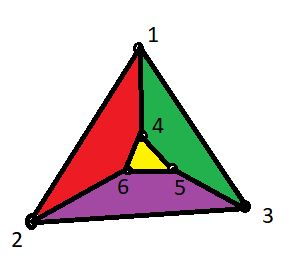
\includegraphics[width=0.5\textwidth]{mapcolor.JPG}
\end{center}
\caption{A graph with 4 regions or faces and each region or face is colored differently}\label{10g8}
\end{figure}

One of the most famous theorems about map coloring states that every planar graph can be map colored with 4 colors. That is, we need only 4 colors to color every region so that no two adjacent regions are colored the same. Here is an example of the map of USA colored with 4 colors. Of course, the region or face in this map are the states of USA. It is not like the normal USA map you see in an atlas; the states are not to-scale. But this map of USA preserves the adjacency relationships. Rishnak asked Ajur can you spot the state of Maine in this Figure \ref{10g9}
\begin{figure}
\begin{center}
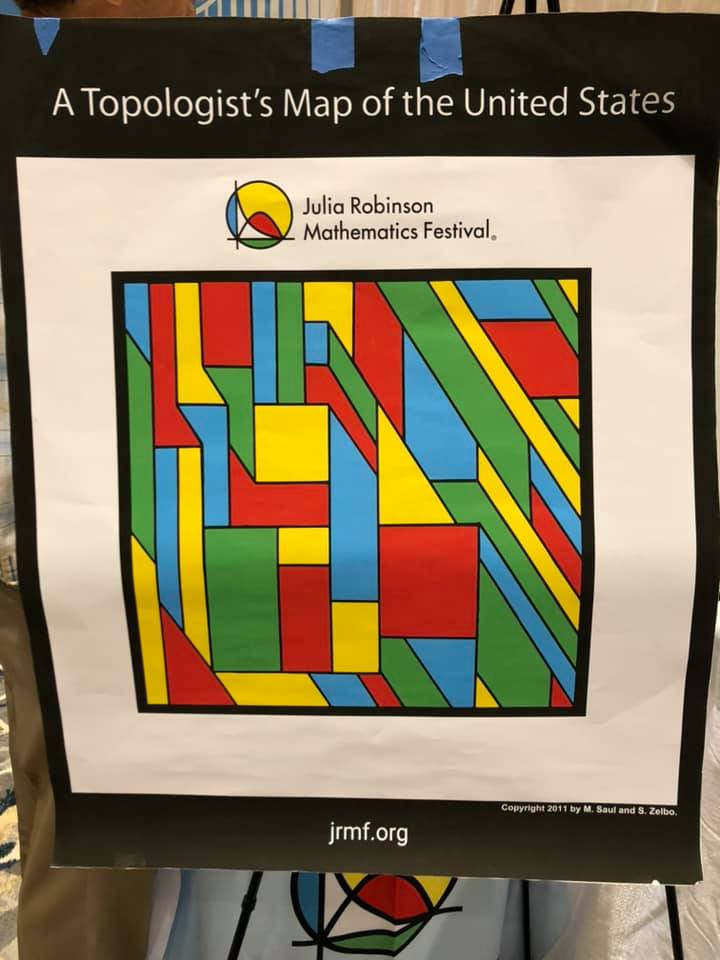
\includegraphics[width=0.5\textwidth]{usamap.png}
\end{center}
\caption{USA Map with faces/states adjacency preserved}\label{10g9}
\end{figure}

Ajur thought for a while. Ajur knew that the state of Maine borders with only one adjacent state that of New Hampshire. So he immediately replied that the region colored yellow in the north east corner is the state of Maine.

Rishnak showed Ajur the map of India with state names given in Figure \ref{10g10}. Rishnak asked Ajur whether the state of Andhra Pradesh and Kerala could be colored the same color?

\begin{figure}
\begin{center}
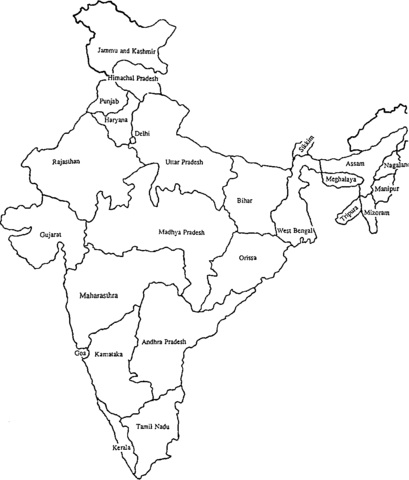
\includegraphics[width=0.9\textwidth]{MapIndia.jpg}
\end{center}
\caption{India Map with faces/states adjacency preserved}\label{10g10}
\end{figure}

Ajur had no hesitation in saying that they could be colored the same color as they share no boundaries or edges. Rishnak asked how about whether Goa and Kerala can be colored the same color. Ajur replied instantaneously with a resounding yes. Ajur asked Rishnak whether the map coloring problem can be converted to a vertex coloring (similar to conversion of edge coloring problem to vertex coloring problem). Ajur further explained that each region/face of the original map would have to become a vertex of the new graph and two vertices in the new graph are adjacent if the corresponding faces in the old graph will share an edge. For example in the continental US map, all the states (faces of the original graph) will become vertices of the new graph and two vertices are adjacent, if the corresponding states share a border in the original graph. For example the vertex corresponding to Maine will be just adjacent to the vertex corresponding to the state of New Hampshire. Similarly, the vertex corresponding to the state of Washington will be adjacent to the vertices corresponding to Oregon and Idaho. Rishnak was very pleased with the way Ajur was absorbing the material. 

\textbf{Question for the eighth day:} Rishnak asked Ajur to color the vertices of the following graph Figure \ref{colorgq1} with as few colors as possible.
\begin{figure}
\begin{center}
\begin{tikzpicture}
  [scale=.6,auto=left,every node/.style={circle}]
  \node (n1) at (0,0) {1};
  \node (n2) at (2,3)  {2};
  \node (n3) at (4,0)  {3};
  \node (n4) at (2,-3) {4};
  \node (n5) at (7,0) {5};
  \node (n6) at (9,3)  {6};
  \node (n7) at (11,0)  {7};
  \node (n8) at (9,-3) {8};



  \foreach \from/\to in {n1/n2,n1/n3,n1/n4,n2/n3,n2/n6, n3/n4, n3/n5, n4/n8, n5/n6,n5/n8,n5/n7,n6/n7,n7/n8}
    \draw (\from) -- (\to);

\end{tikzpicture}

\caption{Color this graph }\label{colorgq1}
\end{center}
\end{figure}

\textbf{Answer: } Ajur has no problem coloring this graph as follows Figure \ref{colorga1}

\begin{figure}
\begin{center}
\begin{tikzpicture}
  [scale=.6,auto=left,every node/.style={circle}]
  \node (n1) [fill=green] at (0,0) {1};
  \node (n2) [fill=red] at (2,3)  {2};
  \node (n3) [fill=blue] at (4,0)  {3};
  \node (n4) [fill=red] at (2,-3) {4};
  \node (n5) [fill=red] at (7,0) {5};
  \node (n6) [fill= green] at (9,3)  {6};
  \node (n7) [fill=blue]  at (11,0)  {7};
  \node (n8) [fill=green] at (9,-3) {8};



  \foreach \from/\to in {n1/n2,n1/n3,n1/n4,n2/n3,n2/n6, n3/n4, n3/n5, n4/n8, n5/n6,n5/n8,n5/n7,n6/n7,n7/n8}
    \draw (\from) -- (\to);

\end{tikzpicture}

\caption{Vertex coloring of graph \ref{colorgq1}}\label{colorga1}
\end{center}
\end{figure}





Rishnak did not want to push further and called it a day. Ajur and Jura were very happy to be left alone. 
\chapter{Spanning Trees}
Rishnak found Ajur and Jura walking along a stretch of road with trees on either side. Recalling his previous talks with Ajur about trees, Rishnak chose a specific kind of tree that is found within a graph for his next session with Ajur.

Rishnak said, ``A graph~$G$ is connected if there is a path between every pair of vertices in~$G$. So, in connected graph~$G=(V,E)$, a \textit{spanning tree} is tree~$T(V,E_1)$ that covers all vertices in~$V$ and is a subgraph of~$G$ that satisfies two conditions:
\begin{enumerate}
    \item Subgraph~$T$ is a tree, meaning it contains no cycles and is connected.
    \item Vertex set~$V$ of~$T$ is the same as that of~$G$.''
\end{enumerate}

Rishnak flashed his hands and formed two graphs in the air in front of Ajur [Figure~\ref{11g1}] [Figure~\ref{11g2}]. He said, ``Here is an example of a graph with a corresponding spanning tree.''

\begin{figure}
\begin{center}
\begin{tikzpicture}
  [scale=.6,auto=left,every node/.style={circle,fill=red!20}]
  \node (n6) at (1,10) {6};
  \node (n4) at (4,8)  {4};
  \node (n5) at (8,9)  {5};
  \node (n1) at (11,8) {1};
  \node (n2) at (9,6)  {2};
  \node (n3) at (5,5)  {3};

  \foreach \from/\to in {n6/n4,n4/n5,n5/n1,n1/n2,n2/n5,n2/n3,n3/n4}
    \draw (\from) -- (\to);

\end{tikzpicture}
\caption{Example graph with six vertices and seven edges}\label{11g1}
\end{center}
\end{figure}

\begin{figure}
\begin{center}
\begin{tikzpicture}
  [scale=.6,auto=left,every node/.style={circle,fill=red!20}]
  \node (n6) at (1,10) {6};
  \node (n4) at (4,8)  {4};
  \node (n5) at (8,9)  {5};
  \node (n1) at (11,8) {1};
  \node (n2) at (9,6)  {2};
  \node (n3) at (5,5)  {3};

  \foreach \from/\to in {n6/n4,n4/n5,n5/n1,n1/n2,n3/n4}
    \draw (\from) -- (\to);

\end{tikzpicture}
\caption{A subgraph of the graph shown in Figure~\ref{11g1} that forms a spanning tree of the original graph}\label{11g2}
\end{center}
\end{figure}

Ajur studied both graphs, recognizing that the second graph was a subgraph of the first.

Rishnak asked Ajur if he could construct another spanning tree for the original graph [Figure~\ref{11g1}].

Ajur was eager to show off and drew a subgraph in the dirt with a stick [Figure~\ref{11g3}].

\begin{figure}
\begin{center}
\begin{tikzpicture}
  [scale=.6,auto=left,every node/.style={circle,fill=red!20}]
  \node (n6) at (1,10) {6};
  \node (n4) at (4,8)  {4};
  \node (n5) at (8,9)  {5};
  \node (n1) at (11,8) {1};
  \node (n2) at (9,6)  {2};
  \node (n3) at (5,5)  {3};

  \foreach \from/\to in {n6/n4,n4/n5,n5/n1,n2/n5,n3/n4}
    \draw (\from) -- (\to);

\end{tikzpicture}
\caption{Another spanning tree of the graph shown in Figure~\ref{11g1}}\label{11g3}
\end{center}
\end{figure}

Rishnak asked, ``How many distinct spanning trees are there?''

Ajur thought about this for a moment. He said, ``Do you mean how many labeled non-isomorphic trees there are?''

Rishnak said, ``Yes, exactly the question?''

Ajur said, ``There are two cycles in this graph, namely~$(2,3,4,5)$ and~$(1,2,5)$, and they share common edge~$(2,5)$. The cycles are of length~4 and length~3, so there are four possible spanning trees to choose from out of the first cycle and three possible spanning trees to choose from out of the other cycle. Multiply these together and we have~12 possibilities, but one of them ends up being cycle~$(1,2,3,4,5)$ if edge~$(2,5)$ is omitted. Therefore, we have~11 spanning trees, each of which must also contain edge~$(4,6)$. Here they are.''

Ajur painstakingly wrote out all~11 spanning trees in the dirt as follows:
\begin{enumerate}
    \item \{(4,6),(4,5),(5,2),(2,3),(5,1)\}
    \item \{(4,6),(4,5),(5,2),(2,3),(2,1)\}
    \item \{(4,6),(4,5),(4,3),(5,2),(5,1)\}
    \item \{(4,6),(4,5),(4,3),(5,2),(2,1)\}
    \item \{(4,6),(4,3),(2,3),(5,2),(5,1)\}
    \item \{(4,6),(4,3),(2,3),(5,2),(2,1)\}
    \item \{(4,6),(4,5),(4,3),(2,3),(5,1)\}
    \item \{(4,6),(4,5),(4,3),(2,3),(2,1)\}
    \item \{(4,6),(4,5),(2,3),(5,1),(1,2)\}
    \item \{(4,6),(4,5),(4,3),(5,1),(1,2)\}
    \item \{(4,6),(4,3),(3,2),(2,1),(1,5)\}
\end{enumerate}

Rishnak nodded and started to speak, but Ajur asked, ``What about the maximum number of labeled spanning trees in a graph with~$n$ vertices? For a complete graph, it must be the maximum number of edges in a graph with~$n$ vertices.''

Rishnak said, ``Correct. Complete graphs have the largest possible number of spanning trees. We can find the number of spanning trees in a complete graph using Pr{\"u}fer codes, which we talked about a few days ago.\footnote{See their discussion in Chapter~8}

Ajur remembered Pr\"ufer codes and said, ``For a tree with~$n$ vertices, we need a Pr{\"u}fer code of length~$n-2$. Each of the~$n-2$ characters in the code could be any of the~$n$ vertices. Therefore, the number of labeled spanning trees in a complete graph with~$n$ vertices has to be~$n^{(n-2)}$.''

Rishnak smiled, then said, ``In general, since there are~$n-1$ edges in a spanning tree, each of the remaining~$e-n+1$ edges, when added to the spanning tree will necessarily create a cycle. Therefore, we will have~$e-n+1$ cycles in the given graph. These cycles are called \textit{fundamental cycles} and, as I have just described, each fundamental cycle has exactly one non-spanning tree edge.\footnote{Euler's equation~(\ref{eqn:euler}) back in Chapter~9 uses this fact.} Let me show you.''

Rishnak waved his hands and the original graph appeared with its edges glimmering in red and blue [Figure~\ref{11g4}]. Rishnak said, ``The blue edges are spanning tree edges, whereas the red edges are non-spanning tree edges that each form a fundamental cycle.''

\begin{figure}
\begin{center}
\begin{tikzpicture}
  [scale=.6,auto=left,every node/.style={circle,fill=red!20}]
  \node (n6) at (1,10) {6};
  \node (n4) at (4,8)  {4};
  \node (n5) at (8,9)  {5};
  \node (n1) at (11,8) {1};
  \node (n2) at (9,6)  {2};
  \node (n3) at (5,5)  {3};

  \foreach \from/\to in {n6/n4,n4/n5,n5/n1,n1/n2,n3/n4}
    \draw [thick,color=blue] (\from) -- (\to);
  \foreach \from/\to in {n5/n2,n2/n3}
   \draw [thick,color=red] (\from) -- (\to);
\end{tikzpicture}
\caption{Original graph from Figure~\ref{11g1} with respect to the spanning tree shown in Figure~\ref{11g2}; here, spanning tree edges are shown as thick blue lines while non-spanning tree edges are shown in red, the latter forming fundamental cycles~$(1,2,5)$ and~$(3,4,5,1,2)$}\label{11g4}
\end{center}
\end{figure}

Ajur wanted to better understand how to find a spanning tree for a given graph, so he asked Rishnak about this.

Rishnak smiled and said, ``First, the graph has to be connected. If that's the case, then it can be done using the following steps:
\begin{enumerate}
\item Start from any vertex. Add that vertex to empty set~$S$.
\item From the vertices in~$S$, find a vertex~$v$ that is not in~$S$ that is adjacent to one of the vertices~$w$ in~$S$. Add that edge~$(v,w)$ to spanning tree~$T$.
\item Repeat Step~2 until all vertices are in~$S$.''
\end{enumerate}

Rishnak formed the original graph again in the air in front of Ajur [Figure~\ref{11g1}]. He said, ``Let me illustrate this. First, add vertex~1 to the set. It has adjacent vertices~2 and~5. Let's say we choose vertex~5 and add it to~$S$. Edge~$(1,5)$ is then the first edge of our spanning tree. From vertices in~$S$, we pick a vertex that is adjacent but not already in~$S$. Choices here are vertices~2 or~4. Let's say we choose vertex~2 and therefore include edge~$(1,2)$ in the spanning tree.''

Ajur said, ``We could have also included edge~$(5,2)$ instead of~$(1,2)$ in the spanning tree, right?''

Rishnak said, ``Yes, the choice is arbitrary. Now, at this point, we have~$S=(1,2,5)$. So we find a vertex not in~$S$ that is adjacent to any of these three vertices. There are two vertices to choose from, namely vertices~3 and~4. Let's say we choose vertex~4 and therefore include edge~$(4,5)$ in the spanning tree.''

Ajur chimed in, ``Now vertices~$(1,2,4,5)$ are in set~$S$. From these vertices, we find a vertex that is adjacent but not in~$S$, so we're looking at vertices~3 and~6. If we choose vertex~3, then we include edge~$(4,3)$ in the spanning tree. Repeating this one more time, we choose vertex~6 and include edge~$(4,6)$ in the spanning tree. And now we're done!''

Rishnak nodded and said, ``Right, now set~$S$ contains all of the vertices, and we have spanning tree~$T$ with edges~$(1,5)$, $(1,2)$, $(5,4)$, $(4,3)$, and $(4,6)$.''---Rishnak waved his hands and the spanning tree from earlier appeared [Figure~\ref{11g2}]---``This is the same spanning tree we came up with earlier.''

Ajur nodded eagerly. He said, ``Aha, and if we had made different choices along the way, we would have ended up with a different spanning tree, like this one.''---Ajur quickly drew another spanning tree in the dirt [Figure~\ref{11g3}].

Rishnak smiled, happy to see that Ajur understood. He said, ``Here is another interesting problem related to spanning trees. As background, a graph is called a \textit{weighted graph} if there are numeric weights or costs associated with each edge. The weight could represent the distance in miles or the cost of travel, and so on.''

Rishnak flashed his hands and the original graph [Figure~\ref{11g1}] appeared, this time with numeric values next to each edge [Figure~\ref{11g7}]. He said, ``Here is an example weighted graph. See each weighted edge?''

\begin{figure}
\begin{center}
\begin{tikzpicture}
  [scale=.6,auto=left,every node/.style={circle,fill=red!20}]
  \tikzstyle{weight} = [fill=none]
  \node (n6) at (1,10) {6};
  \node (n4) at (4,8)  {4};
  \node (n5) at (8,9)  {5};
  \node (n1) at (11,8) {1};
  \node (n2) at (9,6)  {2};
  \node (n3) at (5,5)  {3};
  \foreach \source /\dest /\weight in {n6/n4/1,n4/n5/2,n5/n1/5,n1/n2/2,n2/n5/3,n2/n3/8,n3/n4/7} 
   \draw (\source) --node[weight] {$\weight$}  (\dest);
\foreach \source /\dest /\weight in {1/3/1} place \weight above of=\path;
  
  \end{tikzpicture}
\caption{The graph shown in Figure~\ref{11g1} with edge weights associated with each edge}\label{11g7}
\end{center}
\end{figure}

Ajur said, ``Yes, but how does this change our spanning tree problem?''

Rishnak saw Ajur's impatience. He said, ``We want to find a \textit{minimum spanning tree} in which the sum of all edge weights in the spanning tree is the smallest possible.''

Ajur said, ``Aha, we can enumerate all spanning trees and for each such spanning tree, compute the sum of the edge weights, then choose the spanning tree with the smallest sum.''

Rishnak smiled and said, ``That will work, though that is what we call a \textit{brute force} method. It can be a good strategy for many problems, but we can often find more efficient methods. In this case, we would like to find a faster method that makes certain choices such that we do not have to consider all possible spanning trees.''

Ajur frowned and said, ``I see. If the graph was much larger, we'd have a lot of work to do if we used a brute force approach.''

Rishnak said, ``Exactly. Do not despair, though. We can modify Step~2 of the procedure that I already described to better select each edge. Here is the modified approach:
\begin{enumerate}
\item Start from any vertex. Add that vertex to empty set~$S$.
\item From the vertices in~$S$, find a vertex~$v$ that is not in~$S$ that is adjacent to one of the vertices~$w$ in~$S$---but make sure that edge~$(v,w)$ has the smallest possible edge weight at that decision point. Add that edge~$(v,w)$ to minimum spanning tree~$T$.
\item Repeat Step~2 until all vertices are in~$S$.''
\end{enumerate}

Ajur decided to work through an example by using the graph that Rishnak had formed in front of him [Figure~\ref{11g7}]. He first drew the vertices of the graph in the dirt. Next, he chose vertex~1 and added it to set~$S$. From the two possible edges incident at vertex~1, he chose vertex~2 and added it to~$S$ since the edge weight for edge~$(1,2)$ was smaller than that of edge~$(1,5)$.

Ajur said, ``Aha, I see! Now that vertices~1 and~2 are in~$S$, of the edges leaving~$S$, edge~$(2,5)$ has the smallest edge weight. Therefore, edge~$(2,5)$ is added to the minimum spanning tree and vertex~5 is added to~$S$. Then, from vertices in~$S$, namely~1, 2 and~5, edge~$(5,4)$ has the smallest edge weight. And this continues until we visit each vertex, which we know by adding each vertex in turn to set~$S$.''---Ajur drew each edge in the dirt as he followed the algorithm through to its end [Figure~\ref{11g8}]---``Set~$S$ contains all of the vertices, so here's the minimum spanning tree!''

\begin{figure}
\begin{center}
\begin{tikzpicture}
  [scale=.6,auto=left,every node/.style={circle,fill=red!20}]
  \tikzstyle{weight} = [fill=none]
  \node (n6) at (1,10) {6};
  \node (n4) at (4,8)  {4};
  \node (n5) at (8,9)  {5};
  \node (n1) at (11,8) {1};
  \node (n2) at (9,6)  {2};
  \node (n3) at (5,5)  {3};
  \foreach \source /\dest /\weight in {n6/n4/1,n4/n5/2,n1/n2/2,n2/n5/3,n3/n4/7} 
   \draw[thick] (\source) --node[weight] {$\weight$}  (\dest);
\foreach \source /\dest /\weight in {1/3/1} place \weight above of=\path;
  
  \end{tikzpicture}
\caption{A minimum spanning tree with a total weight of~15 for the weighted graph given in Figure~\ref{11g7}}\label{11g8}
\end{center}
\end{figure}

Rishnak laughed as Ajur could barely control his enthusiasm. Ajur exclaimed, ``We could also use this algorithm to minimally connect a given set of points in a plane. Vertices would correspond to the points. And the distances between each of these points could simply be the length of the straight lines joining them.''

Ajur showed his work in Figure~\ref{11g9}.

\begin{figure}
\begin{center}
\begin{tikzpicture}
  [scale=1,auto=left,every node/.style={circle,fill=red!20}]
  \tikzstyle{weight} = [fill=none]
  \node (n1) at (1,9)  {1};
  \node (n2) at (5,9)  {2};
  \node (n3) at (5,5)  {3};
  \node (n4) at (1,5)  {4};
  \foreach \source /\dest /\weight in {n1/n2/4,n2/n3/4,n3/n4/4} 
   \draw[thick] (\source) --node[weight] {$\weight$}  (\dest);
\foreach \source /\dest /\weight in {1/3/1} place \weight above of=\path;
  \foreach \source /\dest /\weight in {n1/n4/4,n1/n3/5.66,n2/n4/5.66} 
   \draw[color=black,thick,dashed] (\source) --node[weight] {$\weight$}  (\dest);
\foreach \source /\dest /\weight in {1/3/1} place \weight below of=\path;
  \end{tikzpicture}
\caption{A minimum spanning tree representation with a total weight of~12 for a set of four points in the plane; here, edges not part of the minimum spanning tree are shown as dashed lines}\label{11g9}
\end{center}
\end{figure}

\begin{figure}
\begin{center}
\begin{tikzpicture}
  [scale=1,auto=left,every node/.style={circle,fill=red!20}]
  \tikzstyle{weight} = [fill=none]
  \node (n1) at (1,9)  {1};
  \node (n2) at (5,9) {2};
  \node (n3) at (5,5)  {3};
  \node (n4) at (1,5)  {4};
  \node (n5) at (2,7) {5};
  \node (n6) at (4,7) {6};
  \foreach \source /\dest /\weight in {n1/n5/2.23,n5/n6/2,n6/n2/2.23,n6/n3/2.23,n5/n4/2.23} 
   \draw[thick] (\source) --node[weight] {$\weight$}  (\dest);
\foreach \source /\dest /\weight in {1/3/1} place \weight below of=\path;
 
  \end{tikzpicture}
\caption{A minimum Steiner tree for the set of four points or vertices shown in Figure~\ref{11g9}; here, Steiner points are vertices~5 and~6}\label{11g10}
\end{center}
\end{figure}

Another ghost named Urpur had been eavesdropping on Rishnak and Ajur. Urpur wanted to show that he was smarter than both Rishnak and Ajur, so he interrupted and said, ``I have an even smarter approach. There is a spanning tree called the Steiner tree\footnote{Named after the Swiss mathematician Jakob Steiner} wherein one is allowed to add Steiner points or vertices that were not present in the original problem. With a clever addition of Steiner points, I can find a spanning tree that is better than the one Ajur found.''

Urpur clapped his hands and a new graph appeared [Figure~\ref{11g10}]. Urpur said, ``You see?''

Rishnak was impressed with Urpur's solution, but sensing that Ajur was feeling jealous of Urpur, Rishnak said, ``Not bad, Urpur. I am sure Ajur would have also come to this solution if I had asked him.''

Ajur nodded in agreement.

%%\newpage
\subsection*{Question for the ninth day}
Rishnak said, ``It is time now for Ajur to try and answer the question for the ninth day. It has multiple parts.''

Ajur's eyes opened wide in excitement.

Rishnak continued, ``Consider a complete graph with with eight vertices and 28~edges. Of these edges, 14 of them have a weight of~1, while the other 14~edges all have a weight of~10. First, how must you assign the weights so as to achieve the smallest possible minimum weight spanning tree? Second, how must you assign the weights so as to achieve the opposite, the largest possible minimum weight spanning tree?''

\textit{Before you turn the page, try to come up with an answer of your own!}

\newpage
\subsection*{Answer for the ninth day}
Ajur started with the first part. He said, ``If there is a cycle that visits all of the vertices---so a cycle of length~8---and each edge weight in the cycle is~1, then the minimum spanning tree has a weight of~7. We can't go smaller than that.''

Rishnak smiled and said, ``Correct. And for the second part?''

Before Ajur could answer, Urpur said, ``The second part is the real question. And the answer is---''

Ajur jumped up and said, ``The answer is~25. The largest minimum spanning tree will have a total weight of~25.''

Rishnak said, ``And how do you know that?''

Ajur said, ``All of the edges incident at a vertex must be of weight~10 or else we would select an edge of length~1 instead.  Since there are eight vertices, the degree of each vertex must be~7, so two of the graph's vertices can entirely have incident edges of weight~10. That uses up the~14 edge weights of~10, and gives us a minimum spanning tree with a total weight of~$10+10+1+1+1+1+1$, which is~$25$.''

Rishnak smiled.

Urpur said, ``That's what I was going to say!''

Rishnak laughed and decided to call it a night.

Jura barked. He was happy now to get Ajur's attention and jumping with joy, left with Ajur.

\chapter{Shortest Paths}
Ajur had found a map of the cemetery. He used it to try to find the best way to go to the water fountain. Then he remembered his recent discussions with Rishnak and excitedly told Jura that by using graph theory methods, they would be able to find a path and maybe even the shortest path to the water fountain.

Rishnak overheard Ajur and realized that a good discussion of paths and shortest paths would be an ideal topic to pursue next.

Rishnak said, ``Consider a graph\footnote{For spanning trees, we consider only undirected graphs; however, for shortest paths we can consider both undirected and directed graphs.} in which you wish to find the shortest path from a specified source vertex to a specified destination vertex. Let's look at this familiar graph.''---Rishnak waved his hands and an undirected graph appeared in front of Ajur [Figure~\ref{12g1}]---``What's the shortest path from vertex~1 to vertex~6?''

\begin{figure}
\begin{center}
\begin{tikzpicture}
  [scale=.6,auto=left,every node/.style={circle,fill=red!20}]
  \node (n6) at (1,10) {6};
  \node (n4) at (4,8)  {4};
  \node (n5) at (8,9)  {5};
  \node (n1) at (11,8) {1};
  \node (n2) at (9,6)  {2};
  \node (n3) at (5,5)  {3};

  \foreach \from/\to in {n6/n4,n4/n5,n5/n1,n1/n2,n2/n5,n2/n3,n3/n4}
    \draw (\from) -- (\to);

\end{tikzpicture}
\caption{Example undirected graph for which we want to find the shortest path from vertex~1 to vertex~6}\label{12g1}
\end{center}
\end{figure}

Ajur jumped up with excitement and said he could easily draw the shortest path from source vertex~1 to destination vertex~6. He grabbed a stick and drew the graph in the dirt, then he showed the shortest path by thickening edges~$(1,5)$, $(5,4)$, and~$(4,6)$ [Figure~\ref{12g2}].

\begin{figure}
\begin{center}
\begin{tikzpicture}
  [scale=.6,auto=left,every node/.style={circle,fill=red!20}]
  \node (n6) at (1,10) {6};
  \node (n4) at (4,8)  {4};
  \node (n5) at (8,9)  {5};
  \node (n1) at (11,8) {1};
  \node (n2) at (9,6)  {2};
  \node (n3) at (5,5)  {3};

  \foreach \from/\to in {n6/n4,n4/n5,n5/n1}
    \draw [line width=2 pt,color=blue] (\from) -- (\to);
\foreach \from/\to in {n3/n4,n3/n2,n2/n1,n2/n5}
    \draw  (\from) -- (\to);

\end{tikzpicture}
\caption{The graph from Figure~\ref{12g1} with the shortest Path (of length~3) shown from vertex~1 to vertex~6 using thick lines}\label{12g2}
\end{center}
\end{figure}

Pleased with Ajur's enthusiasm, Rishnak wanted to make sure that Ajur understood a general method for finding the shortest path from a source vertex to a destination vertex in any graph.

Rishnak said, ``Remember how to find a spanning tree for a given graph?''

Ajur said, ``Sure, yes.''

Rishnak said, ``Good. We can come up with a similar algorithm for finding the shortest path from a source vertex to a destination vertex, but first, we need to define distance \textbf{dist} of a vertex~$y$ as the number of vertices we must visit to get from the source vertex to vertex~$y$. We also define parent~\textbf{p} of a vertex as the parent vertex\footnote{You can also think of this as the \textit{previous} vertex.} that led us to vertex~$y$. Given these definitions, here is the algorithm:
\begin{enumerate}
\item Set \textbf{dist} for the source vertex to~0 (since the distance from the source vertex to itself is zero). Also set~\textbf{p} as being undefined.
\item Set both \textbf{dist} and~\textbf{p} for all other vertices as being undefined.
\item We start from the source vertex, so add that vertex to a queue.\footnote{In a queue, we can only add elements to the end and remove elements from the front, just like waiting in line at a grocery store. We can also inspect elements in the queue without changing their order.}
\item Remove the vertex from the front of the queue, calling this vertex~$w$. Find all vertices with undefined \textbf{dist} values that are adjacent to~$w$ and put them in set~$A$. Set \textbf{dist} for all of these vertices to be one more than the \textbf{dist} value for~$w$; also set~\textbf{p} to be vertex~$w$. Finally, add all vertices from set~$A$ to the queue.
\item Repeat Step~4 until the destination vertex has its \textbf{dist} value changed, meaning our algorithm has reached the destination vertex. We can then trace the shortest path back to the source vertex by following the~\textbf{p} vertices until we reach the source vertex.''
\end{enumerate}

Ajur knew this was a lot to try to understand. He used the example graph still in front of him [Figure~\ref{12g1}], tracing the algorithm from source vertex~1. He said, ``Okay, so we start by letting the distance \textbf{dist} of vertex~1 be~0, then we add vertex~1 to the queue. We remove vertex~1 from the queue. It has adjacent vertices~2 and~5, so the \textbf{dist} values of these vertices are both set to~2. And vertices~2 and~5 are added to the queue, say with vertex~2 at the end of the queue. Also, the parent~\textbf{p} vertices of vertices~2 and~5 are both set to vertex~1.''

Rishnak said, ``Correct. Keep going.''

Ajur went on, ``Next, we remove vertex~5 from the queue. The only adjacent vertex with an undefined \textbf{dist} value is vertex~4, so we add it to the end of the queue. And we set the \textbf{dist} of vertex~4 to be~2 and the parent~\textbf{p} of vertex~4 to be vertex~5.''

Ajur thought for a moment, then said, ``The first element of the queue is now vertex~2, which we remove next. Next, we add the only adjacent vertex---vertex~3---to the queue. For vertex~3, we set \textbf{dist} to~2 (because it is one more than the \textbf(dist) value of vertex~2) and the parent \textbf{p} to vertex~2. Finally, we remove vertex~4 from the queue and therefore reach vertex~6, which we add to the queue. We set the \textbf{dist} of vertex~6 to be~3 and its parent \textbf{p} to vertex~4. And since vertex~6 is the destination vertex, we're done. The distance from vertex~1 to vertex~6 is~3, and we can work backwards to determine the path since \textbf{p}$(6)=4$, \textbf{p}$(4)=5$, and~\textbf{p}$(5)=1$, which is the source vertex.''

Ajur marveled at the systematic procedure that could be applied to any graph. He also realized that this procedure could be used to find the shortest path from a single source to all other vertices in a given graph. As he thought about this further, he said, ``And we could use this same algorithm to find the shortest paths between every pair of vertices in a graph.''

Rishnak smiled and said, ``There is a graph parameter called the \textit{diameter} of a graph. The diameter is the longest path from among the shortest paths between every pair of vertices. For the example graph we have been using [Figure~\ref{12g1}], the diameter is~3 since the shortest paths between every pair of vertices are of lengths~1, 2, and~3.''

Ajur nodded.

Rishnak flashed his hands and the original graph morphed into a new graph with two fewer edges [Figure~\ref{12g3}].  He said, ``Find the diameter of this graph, Ajur.''

\begin{figure}
\begin{center}
\begin{tikzpicture}
  [scale=.6,auto=left,every node/.style={circle,fill=red!20}]
  \node (n6) at (1,10) {6};
  \node (n4) at (4,8)  {4};
  \node (n5) at (8,9)  {5};
  \node (n1) at (11,8) {1};
  \node (n2) at (9,6)  {2};
  \node (n3) at (5,5)  {3};
   
  \foreach \from/\to in {n6/n4,n4/n5,n1/n2,n2/n3,n3/n4}
    \draw (\from) -- (\to);

\end{tikzpicture}
\caption{An example graph for which we wish to find the diameter}\label{12g3}
\end{center}
\end{figure}

Ajur studied the graph and said, ``Okay, this is the same graph but without edges~$(1,5)$ and~$(2,5)$. I see that this graph is a tree since there are no cycles in the graph. The longest path among all of the shortest paths is from vertex~1 to vertex~5---no wait, there's also a longest path from vertex~1 to vertex~6. Both of them are of length~4, so that's the diameter of this graph.  And therefore, there can be more than one path representing the diameter.''

Rishnak nodded and said, ``Correct. In general, a simple path with~$n$ vertices''---he waved his hands and a new graph appeared [Figure~\ref{12g4}]---``will have a diameter of~$n-1$. And for a complete graph\footnote{Remember that in a complete graph, there is an edge between every pair of vertices.} with~$n$ vertices, the diameter is always~$1$, as the shortest path between every pair of vertices is~$1$.''

Ajur again nodded.

Rishnak asked Ajur, ``Can you construct graphs, all with~$n$ vertices, that have diameters~$n-1,n-2,\ldots,2,\text{ and }1$?''

Ajur thought about this for a few moments. He said, ``Yes, that's not too hard. We already have the graph with a diameter of~$n-1$. Here's a graph with a diameter of~$n-2$''---he drew a graph in the dirt [Figure~\ref{12g5}]---``and another with diameter~$2$.''---he quickly drew another graph [Figure~\ref{12g6}].

Ajur smiled broadly and said, ``From these two graphs, you can infer the rest!''

\begin{figure}
\begin{center}
\begin{tikzpicture}
  [scale=.6,auto=left,every node/.style={circle,fill=red!20}]
  \node (n1) at (1,8) {$1$};
  \node (n2) at (3,8)  {$2$};
  \node (n3) at (5,8)  {$.$};
  \node (n4) at (7,8) {$.$};
  \node (n5) at (9,8)  {$.$};
  \node (n6) at (11,8)  {$n$};
   
  \foreach \from/\to in {n1/n2,n2/n3,n3/n4,n4/n5,n5/n6}
    \draw (\from) -- (\to);

\end{tikzpicture}
\caption{A graph with~$n$ vertices will always have a diameter of~$n-1$}\label{12g4}
\end{center}
\end{figure}

\begin{figure}
\begin{center}
\begin{tikzpicture}
  [scale=.6,auto=left,every node/.style={circle,fill=red!20}]
  \node (n1) at (1,8) {$n$};
  \node (n2) at (3,8)  {$.$};
  \node (n3) at (5,8)  {$.$};
  \node (n4) at (7,8) {$.$};
  \node (n5) at (9,10)  {2};
  \node (n6) at (9,8)  {1};
   
  \foreach \from/\to in {n1/n2,n2/n3,n3/n4,n4/n5,n4/n6}
    \draw (\from) -- (\to);

\end{tikzpicture}
\caption{A graph with~$n$ vertices with a diameter of~$n-2$}\label{12g5}
\end{center}
\end{figure}
\begin{figure}
 \begin{center}
\begin{tikzpicture}
  [scale=.6,auto=left,every node/.style={circle,fill=red!20}]
  \node (n1) at (1,8) {$n$};
  \node (n2) at (1,10)  {$.$};
  \node (n3) at (3,8)  {$.$};
  \node (n4) at (1,6) {$.$};
  \node (n5) at (-1,6)  {2};
  \node (n6) at (-2,8)  {1};
   
  \foreach \from/\to in {n1/n2,n1/n3,n1/n4,n1/n5,n1/n6}
    \draw (\from) -- (\to);

\end{tikzpicture}
\caption{A graph with~$n$ vertices with a diameter of~$2$}\label{12g6}
\end{center}
\end{figure}

Rishnak said, ``Here is another interesting problem. Can we construct a regular undirected graph with given diameter~$k$?''

Ajur shrugged his shoulders and said, ``But how many vertices?''

Rishnak smiled as he continued, ``Yes, Ajur, an answer here is a set of graphs called \textit{Moore} graphs. In addition to diameter~$k$, we define degree~$d$ for the graph, meaning that each vertex has degree~$d$. Then we can calculate the number of vertices in the graph using this formula.''

Rishnak flashed his hands and the following formula appeared in the air in front of Ajur:
$$\text{number of vertices} = 1+\sum_{i=1}^{k-1} (d-1)^i$$

Ajur frowned as he studied the formula.

Rishnak said, ``Let me explain. We can understood this formula by drawing a graph in the shape of a rooted tree of depth~$k-1$''---Rishnak waved his hands and a new graph appeared [Figure~\ref{12g7}]---``which we have already seen.\footnote{This is the Petersen graph from Figure~\ref{5g4}.} In this graph, the root vertex has~$d$ children and every other vertex has~$d-1$ children. All of the leaf vertices break the tree properties since they are connected in such a way that every vertex has degree~$d$.''

Ajur studied this graph and said, ``Aha, and this graph's diameter is~$k$.''

Rishnak smiled and said, ``Precisely.''

\begin{figure}
\begin{center}
\begin{tikzpicture}[scale=0.7, every node/.style={circle,fill=red!10},level/.style={sibling distance=60mm/#1}]
\node [circle,draw] (z){$1$}
  child {node [circle,draw] (a) {$2$}
    child {node [circle,draw] (b) {$3$}}
    child {node [circle,draw] (c) {$7$}}}
    child {node [circle,draw] (d) {$5$}
        child {node [circle,draw] (e) {$4$}}
        child {node [circle,draw] (f) {$10$}}}
    child {node [circle,draw] (g) {$6$}
        child {node [circle,draw] (h) {$8$}}
        child {node [circle,draw] (i) {$9$}}};
\path
(b) edge [bend right] (h)
(b) edge [bend right] (e)
(c) edge [bend right] (i)
(c) edge [bend right] (f)
(e) edge [bend right] (i)
(f) edge (h)
;
\end{tikzpicture}
\caption{The Petersen graph from Figure~\ref{5g4} drawn in the shape of a rooted tree with a diameter of~$2$ and a degree of~$3$}\label{12g7}
\end{center}
\end{figure}

Ajur thought for a few moments, wondering about weighted graphs.  He said, ``Is there an algorithm to find shortest paths in weighted graphs?\footnote{Remember a weighted graph is a graph with weights or costs associated with each edge.}

Rishnak said, ``Yes, Ajur, good thinking.''  Rishnak waved his hands and a weighted graph appeared in the air [Figure~\ref{12g8}].

Rishnak continued, ``We can modify the shortest path algorithm from earlier to work for weighted graphs. Remember from that algorithm that we aim to find the shortest path from a source vertex to a destination vertex.  Then we redefine distance \textbf{dist} of a vertex~$y$ as the minimum sum of the weights along the edges we used to get from the source vertex to vertex~$y$. We still have parent~\textbf{p} of a vertex as the parent vertex that led us to vertex~$y$. Given these revised definitions, here is the algorithm:
\begin{enumerate}
\item Set \textbf{dist} for the source vertex to~0 (since the distance from the source vertex to itself is zero). Also set~\textbf{p} as being undefined.  Further, set \textbf{explored} to~$1$.
\item For all other vertices, set \textbf{dist} to~$\infty$, set \textbf{explored} to~$0$, and set~\textbf{p} as being undefined.
\item We start from the source vertex, so add that vertex to a queue.
\item Remove the vertex from the front of the queue, calling this vertex~$w$. Find all vertices with \textbf{explored} set to~$0$ that are adjacent to~$w$ and put them in set~$A$. For each vertex~$v\in A$, set its \textbf{dist} value to the minimum of the \textbf{dist} value for~$v$ and the sum of the \textbf{dist} value for~$w$ plus the weight of edge~$(w,v)$. If we use the sum here, then also set~\textbf{p} for vertex~$v$ to be~$w$ (since we found a shorter path).
\item Add the vertex with the smallest \textbf{dist} value from set~$A$ to the queue, also setting its \textbf{explored} value to~$1$.
\item Repeat Steps~4 and~5 until the destination vertex has its \textbf{dist} value changed, meaning our algorithm has reached the destination vertex. We can then trace the shortest path back to the source vertex by following the~\textbf{p} vertices until we reach the source vertex.''
\end{enumerate}


\begin{figure}
\begin{center}
\begin{tikzpicture}
  [scale=.6,auto=left,every node/.style={circle,fill=red!20}]
  \tikzstyle{weight} = [fill=none]
  \node (n6) at (1,10) {6};
  \node (n4) at (4,8)  {4};
  \node (n5) at (8,9)  {5};
  \node (n1) at (11,8) {1};
  \node (n2) at (9,6)  {2};
  \node (n3) at (5,5)  {3};
  \foreach \source /\dest /\weight in {n6/n4/1,n4/n5/2,n5/n1/5,n1/n2/2,n2/n5/2,n2/n3/8,n3/n4/7} 
   \draw (\source) --node[weight] {$\weight$}  (\dest);
\foreach \source /\dest /\weight in {1/3/1} place \weight above of=\path;
  
  \end{tikzpicture}
\caption{A weighted graph with six vertices and seven edges for which we wish to find the shortest path from vertex~1 to vertex~6}\label{12g8}
\end{center}
\end{figure}

Ajur studied the graph in front of him, then drew it in the dirt.  He said, ``Okay, let me try to use the algorithm on this graph. Initially, \textbf{dist} of vertex~1 is set to~$0$, and for the rest of the vertices, \textbf{dist} is set to~$\infty$. Also, \textbf{explore} of vertex~1 is~$1$ since we have explored that vertex and~$0$ for the rest of the vertices. Scanning from vertex~1, \textbf{dist} of vertex~5 is~5 and \textbf{dist} of vertex~2 is~2. So the \textbf{p} labels of vertices~2 and~5 are both set to refer back to vertex~$1$.''

Rishnak said, ``Good, Ajur, that is a good start, yes.''

Ajur continued, ``Then we have to choose which vertex to explore next by selecting the adjacent vertex with the smallest \textbf{dist} value. That would be vertex~2, so we set \textbf{explore} for vertex~2 to~1. Next, we update \textbf{dist} of vertex~5 to~4 (since the sum~$2+2$ is less than~5) and \textbf{dist} of vertex~3 to~10. We also set their \textbf{p} values to both be vertex~2. We then select vertex~5 and set its \textbf{explore} value to~1. From vertex~5, \textbf{dist} of vertex~4 is set to~6 and its parent label is set to vertex~5.''---Ajur sighed as this was getting quite tedious---``Okay, then we go to vertex~4 so we set its \textbf{explore} label to~1. From vertex~4, \textbf{dist} of vertex~6 becomes 7 and its \textbf{p} value refers to vertex~4. In this case, \textbf{dist} of vertex~3 does not change. So finally, we set \textbf{explore} of vertex~6 to~1 and since it is the destination vertex, the algorithm stops.''

Ajur stepped back and looked again at the graph he had drawn [Figure~\ref{12g9}].  He said, ``We then know that the shortest path from vertex~1 to vertex~6 is of length~7. The path can be traced backward from vertex~6 through the \textbf{p} values, so we have \textbf{p}$(6)=4$, \textbf{p}$(4)=5$, \textbf{p}$(5)=2$, and~\textbf{p}$(2)=1$, the source vertex.''

\begin{figure}
\begin{center}
\begin{tikzpicture}
  [scale=.6,auto=left,every node/.style={circle,fill=red!20}]
  \tikzstyle{weight} = [fill=none]
  \node (n6) at (1,10) {6};
  \node (n4) at (4,8)  {4};
  \node (n5) at (8,9)  {5};
  \node (n1) at (11,8) {1};
  \node (n2) at (9,6)  {2};
  \node (n3) at (5,5)  {3};
  \foreach \source /\dest /\weight in {n5/n1/5,n2/n3/8,n3/n4/7} 
   \draw (\source) --node[weight] {$\weight$}  (\dest);
\foreach \source /\dest /\weight in {1/3/1} place \weight above of=\path;
  \foreach \source /\dest /\weight in {n6/n4/1,n4/n5/2,n1/n2/2,n2/n5/2} 
   \draw[line width=2 pt,color=blue] (\source) --node[weight] {$\weight$}  (\dest); 
  \end{tikzpicture}
\caption{The weighted graph from Figure~\ref{12g8} with the shortest path from vertex~1 to vertex~6 shown using thick lines}\label{12g9}
\end{center}
\end{figure}

Rishnak smiled as Ajur appreciated the power of the algorithm, knowing now that he could use this algorithm to compute the shortest route from the cemetery entrance to the water fountain---or anywhere else!

\subsection*{Question for the tenth day}
Rishnak said, ``It is now time for the question for the tenth day, Ajur. There are two parts to this question. Using the graph you have just seen [Figure~\ref{12g9}], first, how can you change the weight of a single edge such that the shortest path from vertex~1 to vertex~6 must go through vertex~3? Second, what is the minimum edge weight for the changed edge to still have the shortest path go through vertex~3?''

\textit{Before you turn the page, try to come up with answers of your own!}

\newpage
\subsection*{Answer for the tenth day}
Ajur thought about changing an edge incident on vertex~1 but quickly found that the shortest path would then simply follow the other vertex (i.e.,~vertex~2 or vertex~5).
After a few moments of pondering, Ajur erased the edge weight for edge~$(5,4)$ and replaced it with a new edge weight of~1000.

Ajur said, ``If the weight of edge~$(5,4)$ is increased to 1000, then the shortest path is forced to go through vertex~3.'' He drew the new shortest path using thick lines to emphasize the path [Figure~\ref{12qa1}].

Rishnak said, ``Good, and what could the minimum edge weight be for edge~$(5,4)$ to still have the shortest path go through vertex~3?''

Ajur said quickly, ``Easy, the shortest path through vertex~3 has a length of~18, so edge~$(5,4)$ would need to have a weight of~14 for the second-shortest path to be~19.''

\begin{figure}
\begin{center}
\begin{tikzpicture}
  [scale=.6,auto=left,every node/.style={circle,fill=red!20}]
  \tikzstyle{weight} = [fill=none]
  \node (n6) at (1,10) {6};
  \node (n4) at (4,8)  {4};
  \node (n5) at (8,9)  {5};
  \node (n1) at (11,8) {1};
  \node (n2) at (9,6)  {2};
  \node (n3) at (5,5)  {3};
  \foreach \source /\dest /\weight in {n5/n1/5,n2/n5/2,n4/n5/1000} 
   \draw (\source) --node[weight] {$\weight$}  (\dest);
\foreach \source /\dest /\weight in {1/3/1} place \weight above of=\path;
  \foreach \source /\dest /\weight in {n6/n4/1,n3/n4/7,n2/n3/8,n1/n2/2} 
   \draw[line width=2 pt,color=blue] (\source) --node[weight] {$\weight$}  (\dest); 
  \end{tikzpicture}
\caption{The weighted graph from Figure~\ref{12g8} with the shortest path from vertex~1 to vertex~6 shown using thick lines, this time going through vertex~3 given the increased edge weight of edge~$(5,4)$}\label{12qa1}
\end{center}
\end{figure}

Rishnak smiled and said, ``Yes, Ajur, very good.''

Ajur wanted to learn more, but he was getting tired and wanted to find the shortest path from where he stood to a bench on which he could lie down and take a nap. So, along with Jura, Ajur walked off in that direction.
\chapter{Cliques, Independent sets and Vertex covering }
Rishnak was eager to discuss other interesting problems with Ajur and  spotted Ajur and Jura walking along the shore of a pond. Rishnak asked Ajur about cliques in his school. Ajur readily shared his pet peeve with Rishank. Yes, students in his school belonged to distinct groups, essentially cliques. Then Rishnak told Ajur that a clique is also a graph theoretic term. A clique is a subgraph of a graph which is complete. Rishnak added that normally we only consider maximal complete subgraphs as cliques, that a maximal complete subgraph of $G$, $H$, means that there is no complete subgraph of $G$ that contains $H$ as a subgraph,

Rishnak drew the following graph in Figure \ref{13g1} and asked Ajur to list the cliques(maximal complete subgraphs).
\begin{figure}
\begin{center}
\begin{tikzpicture}
  [scale=.6,auto=left,every node/.style={circle,fill=red!20}]
  \node (n6) at (1,10) {6};
  \node (n4) at (4,8)  {4};
  \node (n5) at (8,9)  {5};
  \node (n1) at (11,8) {1};
  \node (n2) at (9,6)  {2};
  \node (n3) at (5,5)  {3};

  \foreach \from/\to in {n6/n4,n4/n5,n5/n1,n1/n2,n2/n5,n2/n3,n3/n4,n4/n2,n3/n5}
    \draw (\from) -- (\to);

\end{tikzpicture}
\caption{ What are the maximal cliques (complete subgraphs) in this graph}\label{13g1}
\end{center}
\end{figure}

Ajur was tentative in his answer - as he was struggling with all the definitions. then stated that the three maximal cliques are: 
\begin{enumerate}
    \item Induced subgraph containing vertices 4 and 6.
    \item Induced subgraph containing the vertices 2,3 4 and 5
    \item Induced subgraph containing the vertices 1, 2 and 5
\end{enumerate} 

Rishnak was happy to note that Ajur understood the definition of maximal cliques. Still he wanted Ajur to find the
maximal cliques on another graph shown in Figure \ref{13g21}.
\begin{figure}
\begin{center}
\begin{tikzpicture}
  [scale=.6,auto=left,every node/.style={circle,fill=red!20}]
  \node (n6) at (1,10) {6};
  \node (n4) at (4,8)  {4};
  \node (n5) at (8,9)  {5};
  \node (n1) at (11,8) {1};
  \node (n2) at (9,6)  {2};
  \node (n3) at (5,5)  {3};

  \foreach \from/\to in {n6/n4,n4/n5,n5/n1,n1/n2,n2/n5,n2/n3,n3/n4,n4/n2,n3/n5,n1/n4,n1/n3,n3/n6,n5/n6}
    \draw (\from) -- (\to);

\end{tikzpicture}
\caption{ What are the maximal cliques (complete subgraphs) in this graph}\label{13g21}
\end{center}
\end{figure}

Ajur stared at the figure \ref{13g21} for a few seconds, then answered, giving two maximal cliques. He listed them as: 
\begin{enumerate}
    \item Induced subgraph containing vertices 3, 4, 5 and 6.
    \item Induced subgraph containing the  some vvertices 1, 2,3 4 and 5.
\end{enumerate} 
Seeing Ajur  frustrated with vague definitions and examples, Rishnak admitted that it was his mistake. Graphs are usually used as models for physical or social processes. For example, when we consider the cliques in a school, one can model the students as vertices and two students belong to the same group as an edge between the associated vertices\footnote{We have a binary relation here.}. Clusters in data science are closely related to cliques. Since graphs are models of social a

Rishnak then wanted Ajur to learn about Independent set in a graph. An independent set in a graph is a set of vertices that are mutually nonadjacent i.e., a subset of vertices that does not include any adjacent vertices. Ajur immediately recognized that Independent set and Clique are related. Rishnak could not control his smile. Rishnak remembered that he had not told Ajur about complement of a graph. A complement of a graph $G=(V,E)$ is another graph $H=(V,E_1)$. Both of them have the same vertex set. But if two vertices are adjacent in G, they are not adjacent in H and if two vertices are not adjacent in G, then they are adjacent in H. Ajur drew the complement of the graph shown in Figure \ref{13g1} as shown in Figure \ref{13g21}

\begin{figure}
\begin{center}
\begin{tikzpicture}
  [scale=.6,auto=left,every node/.style={circle,fill=red!20}]
  \node (n6) at (1,10) {6};
  \node (n4) at (4,8)  {4};
  \node (n5) at (8,9)  {5};
  \node (n1) at (11,8) {1};
  \node (n2) at (9,6)  {2};
  \node (n3) at (5,5)  {3};

  \foreach \from/\to in {n6/n5,n6/n3,n6/n2,n6/n1, n1/n3,n1/n4}
    \draw (\from) -- (\to);

\end{tikzpicture}
\caption{ Complement of Graph in \label{13g1}}\label{13g2}
\end{center}
\end{figure}

Ajur further said that the number of edges in the complement of the graph will be $n\times\frac{n-1}{2}-e$ where original graph has $n$ 
vertices and $e$ edges. Hence a maximal clique in a graph will be an independence set in the 
complement of the graph. For the graph shown in Figure \ref{13g2}, the maximal independence sets are $\{2,3,4,5\}, \{1,2,5\} , \{4,6\}$ \footnote{Maximal here means that a super-set of it cannot be an independent set}. 
These are also the maximal cliques in Figure \ref{13g1}. In a bipartite graph shown below \ref{13g3}, the maximal independent sets are $\{1,2\}, \{3,4,5,6\}, \{2,6\}$.

\begin{figure}
\begin{center}
\begin{tikzpicture}
  [scale=.3,auto=left,every node/.style={circle,fill=red!20}]
  \node (n1) at (1,7) {1};
  \node (n2) at (5,7)  {2};
  \node (n3) at (1,2)  {3};
  \node (n4) at (5,2) {4};
  \node (n5) at (9,2)  {5};
   \node (n6) at (13,2) {6};
  
   \foreach \from/\to in {n1/n3,n1/n4,n1/n5,n2/n3,n2/n4,n2/n5,n1/n6}
    \draw (\from) -- (\to);
    \end{tikzpicture}
\caption{ A Bipartite Graph with 6 vertices and 7 edges}\label{13g3}
\end{center}
\end{figure}

Finding a maximal independent set is not hard, finding a maximum independent set is very hard - similar to finding a maximum clique. Maximum independent set refers to the maximal independent set which has the largest size. For the graph in Figure \ref{13g2}. the maximum independent set is $\{2,3,4,5\}$. For the graph in Figure \ref{13g3}, the maximum independent set is $\{3,4,5,6\}$.  Rishnak said that it is easy to find the maximum independent set in a tree. Ajur jumped up and down and said the he had a solution and described the following procedure. Ajur said that the input to his procedure is a rooted tree and the output is the maximum independent set.

Ajur also showed his procedure on the following example Figure \ref{13g4}
\begin{enumerate}
    \item Let Maximum Independent set, $X=\emptyset$
    \item Add all the leaf vertices to a maximum independent set $X$.
    \item Delete all the leaf vertices \footnote {Deletion of a vertex means delete a vertex and delete all the edges incident on that vertex}
    \item Delete all the newly created leaf vertices if there are any.
    \item Go to step 2, if the tree is not empty.
    \item $X$ is the maximum independent set of a tree.
\end{enumerate}

\begin{figure}
\begin{center}

\begin{tikzpicture}
  [scale=.6,auto=left,every node/.style={circle,fill=red!20}]
  \node (n1) at (5.5,7) {1};
  \node (n2) at (3,5)  {2};
  \node (n3) at (8,5)  {3};
  \node (n4) at (2,3) {4};
  \node (n5) at (4,3)  {5};
  \node (n6) at (7,3)  {6};
  \node (n7) at (9,3)  {7};

  \foreach \from/\to in {n1/n2,n1/n3,n2/n4,n2/n5,n3/n6,n3/n7}
    \draw (\from) -- (\to);

\end{tikzpicture}
\caption{ The maximum independent set is $\{4,5,6,7,1\}$}\label{13g4}
\end{center}
\end{figure}

A closely related to Independent set is Vertex Cover. A vertex cover of a graph is a minimal subset of vertices that cover all the edges of a graph. Alternatively, if you delete all the elements in a vertex cover, the remaining graph will be an empty graph (that is a graph with no edges). Intuitively, if we place policewomen in all the vertices of the vertex cover, then the policewomen will be able to watch all the edges (may be roads or corridors). Since we wanted to employ as few policewomen as possible, we want a minimal vertex cover.\footnote{minimal vertex cover means that no subset of it is also a vertex cover}
\begin{figure}
\begin{center}

\begin{tikzpicture}
  [scale=.6,auto=left,every node/.style={circle,fill=red!20}]
  \node (n1) at (5.5,7) {1};
  \node (n2) at (3,5)  {2};
  \node (n3) at (8,5)  {3};
  \node (n4) at (2,3) {4};
  \node (n5) at (4,3)  {5};
  \node (n6) at (7,3)  {6};
  \node (n7) at (9,3)  {7};

  \foreach \from/\to in {n1/n2,n1/n3,n2/n4,n2/n5,n3/n6,n3/n7}
    \draw (\from) -- (\to);

\end{tikzpicture}
\caption{ The minimal vertex cover  is $\{2,3\}$ as all edges are incident on either 2 or 3}\label{13g5}
\end{center}
\end{figure}

Ajur said that vertex cover and independent set seem to be related. Rishnak smiled ad replied if $X$ is a maximal independent set in a graph with $V$ as vertex set, then $V-X$ is a minimal vertex cover. Similarly if $Y$ is a maximum independent set and $V-Y$ is a minimum vertex cover. Ajur was impressed how all these seemingly unrelated sets are actually related. Ajur thought for a while and he said he understood how maximal independent set and minimal vertex cover are related. Maximal independent set,$X$, contains no edges as per definition. This implies that vertex set  $V-X$ covers all edges of the graph or every edge is incident in some vertex of $V-X$.

Rishnak wanted to test Ajur's understanding. He said that in olden days temples were constructed at the junctions of roads in a village. He asked Ajur, for the smallest number of temples that had to be constructed in the following Figure \ref{13g6} which shows the road map of Royt so that there is at least temple at either end of each edge..
\begin{figure}
\begin{center}

\begin{tikzpicture}
  [scale=.6,auto=left,every node/.style={circle,fill=red!20}]
  \node (n1) at (6,-3) {1};
  \node (n2) at (0,3)  {2};
  \node (n3) at (2,3)  {3};
  \node (n4) at (4,1) {4};
  \node (n5) at (8,1)  {5};
  \node (n6) at (12,3)  {6};
  \node (n7) at (6,3)  {7};
 \node (n8) at (10,3) {8};
  \node (n9) at (4,5)  {9};
  \node (n10) at (8,5)  {10};
  \node (n11) at (6,8)  {11}; 

  \foreach \from/\to in {n1/n2,n1/n4,n1/n5,n1/n6,n2/n3,n2/n11,n3/n4,n3/n9,n4/n7,n5/n7,n5/n8,n6/n8,n6/n11,n7/n9,n7/n10,n8/n10,n9/n11,n10/n11}
    \draw (\from) -- (\to);

\end{tikzpicture}
\caption{ Royt Village Road Map}\label{13g6}
\end{center}
\end{figure}

Ajur was mesmerized by the beautiful layout of Royt village. It looked so symmetric. He was tentative in his answer and he said that he would construct just 5 temples in vertices 11, 3, 7, 8 and 1.   When asked how he found so quickly. Ajur responded saying that he tried to find a minimum vertex cover for the Figure \ref{13g6} and he knew that would satisfy the temple requirements.

Rishnak was impressed. It was getting dark and both of them called it a night.

\chapter{Bridges, Cut Vertices, Cutsets}

Remembering that he had not told Ajur about some concepts related to connectivity of graphs and directed graphs, Rishnak went looking for Ajur and saw Ajur and Jura walking on a bridge over a small brook. Rishnak gently tapped Ajur and said that 
he wanted to talk about connectivityy. Ajur replied saying he remembered the definition of being connected - which means that there is a path between every pair of vertices. Rishnak smiled and said that it is correct.

A bridge is an edge in a connected graph that when that edge is deleted from that graph, it becomes disconnected. For the graph shown in Figure \ref{14g1}, every edge is bridge.
\begin{figure}
\begin{center}

\begin{tikzpicture}
  [scale=.6,auto=left,every node/.style={circle,fill=red!20}]
  \node (n1) at (5.5,7) {1};
  \node (n2) at (3,5)  {2};
  \node (n3) at (8,5)  {3};
  \node (n4) at (2,3) {4};
  \node (n5) at (4,3)  {5};
  \node (n6) at (7,3)  {6};
  \node (n7) at (9,3)  {7};

  \foreach \from/\to in {n1/n2,n1/n3,n2/n4,n2/n5,n3/n6,n3/n7}
    \draw (\from) -- (\to);

\end{tikzpicture}
\caption{ Every edge in this graph is a bridge. In a tree, every edge is bridge!}\label{14g1}
\end{center}
\end{figure}

In the graph shown in Figure \ref{14g2}, just one edge is a bridge.

\begin{figure}
\begin{center}
\begin{tikzpicture}
  [scale=.6,auto=left,every node/.style={circle,fill=red!20}]
  \node (n6) at (1,10) {6};
  \node (n4) at (4,8)  {4};
  \node (n5) at (8,9)  {5};
  \node (n1) at (11,8) {1};
  \node (n2) at (9,6)  {2};
  \node (n3) at (5,5)  {3};

  \foreach \from/\to in {n6/n4,n4/n5,n5/n1,n1/n2,n2/n5,n2/n3,n3/n4}
    \draw (\from) -- (\to);

\end{tikzpicture}
\caption{Edge (4,6) is the bridge}\label{14g2}
\end{center}
\end{figure}

Bridge is an important edge in a graph. If the bridge is deleted (if it fails), the graph becomes disconnected. A graph may not contain any bridge. For example, in a complete graph  there are no
bridges. If there are no bridges, there is less chance that a graph becomes disconnected when an edge is deleted.

Ajur asked Rishnak whether there is a vertex analog of a bridge. Rishnak answered in the affirmative. A cut-vertex is a vertex which when deleted \footnote{deleting a vertex means removing that vertex and removing all edges incident on that vertex.} makes the graph disconnected. In the graph shown in \ref{14g2}, vertex 4 is a cut vertex. If you consider the map of continental United States (with states as vertices and there is an edge between two vertices (states), if they share a common border), New Hampshire is a cut-vertex, if you delete New Hampshire, it is not possible to go from Maine to other states through United States. Similarly in India, West Bengal is  a cut vertex, as from north eastern state (like Assam), you cannot go to Kerala!

In a tree, all vertices other than leaf vertices are cut vertices. In a complete graph, there are no cut vertices. If a graph or a network has a cut vertex, that network is vulnerable and may get disconnected if the cut vertex fails. 

A graph is $k$ connected if there is a set of $k$ vertices which when deleted from the graph becomes disconnected. Ajur realized that $k$ connected is a generalization of 1 connected (correspond to having a cut vertex.)

A cutset is a set of edges which when deleted will make the graph disconnected. Rishnak asked Ajur how many vertices need to be deleted for the graph shown in Figure \ref{14g3} and what is a cutset for this graph.

\begin{figure}
\begin{center}

\begin{tikzpicture}
  [scale=.6,auto=left,every node/.style={circle,fill=red!20}]
  \node (n1) at (6,-3) {1};
  \node (n2) at (0,3)  {2};
  \node (n3) at (2,3)  {3};
  \node (n4) at (4,1) {4};
  \node (n5) at (8,1)  {5};
  \node (n6) at (12,3)  {6};
  \node (n7) at (6,3)  {7};
 \node (n8) at (10,3) {8};
  \node (n9) at (4,5)  {9};
  \node (n10) at (8,5)  {10};
  \node (n11) at (6,8)  {11}; 

  \foreach \from/\to in {n1/n2,n1/n4,n1/n5,n1/n6,n2/n3,n2/n11,n3/n4,n3/n9,n4/n7,n5/n7,n5/n8,n6/n8,n6/n11,n7/n9,n7/n10,n8/n10,n9/n11,n10/n11}
    \draw (\from) -- (\to);

\end{tikzpicture}
\caption{How many vertices should be deleted to make this graph disconnected? How many edges should be deleted to make this graph disconnected? }\label{14g3}
\end{center}
\end{figure}

Ajur said in a hurry that by deleting vertices 1,3, 11, the graph in \ref{14g3} will be disconnected. He
also gave a cutset consisting of edges (2,3),(2,11) and (1,2).

\textbf{Question for twelfth day:}  What is the largest number of bridges one can have in a connected graph with $n$ vertices, Draw a graph with six vertices, having exactly two bridges.

\textbf{Answer:} Ajur said that a tree is a minimally connected graph. Since every edge is in some unique path, all the edges of the tree are bridges. Hence the maximum number of bridges in a connected graph can be $n-1$. If we have $n$ or more edges, then we will have a cycle. Hence we cannot have bridges $\ge~n$.

Ajur drew the following graph Figure \ref{14ag1} which has exactly two bridges with six vertices.

\begin{figure}
\begin{center}
\begin{tikzpicture}
  [scale=.6,auto=left,every node/.style={circle,fill=red!20}]
  \node (n6) at (1,10) {6};
  \node (n4) at (4,8)  {4};
  \node (n5) at (8,9)  {5};
  \node (n1) at (11,8) {1};
  \node (n2) at (9,6)  {2};
  \node (n3) at (5,5)  {3};

  \foreach \from/\to in {n6/n4,n3/n5,n5/n1,n1/n2,n2/n5,n2/n3,n3/n4}
    \draw (\from) -- (\to);

\end{tikzpicture}
\caption{A graph with six vertices and two bridges (6,4) and (4,3)}\label{14ag1}
\end{center}
\end{figure}


Rishnak noticed that Ajur and Jura were getting impatient and called it a night.
\chapter{Strongly Connected Directed Graphs}
Rishnak was anxious to meet Ajur as he remembered that he had not discussed about directed graphs that much. 
Luckily Rishnak found Ajur walking near a lonely path with Jura. Rishnak asked Ajur whether Ajur remembered about relations. Ajur replied that the relation could be symmetric like a facebook friend (that is if A is a friend of B, then B is also a friend of A - resulting in a friendship
undirected graph.
The relation can also be asymmetric -like a twitter follower (that is if X follows the twitter
feed of Y, Y need not follow the twitter feed of X) - resulting in a twitter directed graph.
Rishnak said that there are many relations which are asymmetric like less than or precedence relations or parent relation or winner relation. In each case, we get a directed graph representing the asymmetric relation.
Similar to path and walk in an undirected graph, we can define path and walk in directed graph (which we discussed in Chapter 6).

An undirected graph is connected if there is a path between every pair of vertices. A directed graph is strongly connected, if there is directed path between every pair of vertices. Rishnak showed the following example Figure \ref{15g1}

\begin{figure}
\begin{center}
\begin{tikzpicture}
  [scale=.8,auto=left,every node/.style={circle,fill=red!10}]
  \node (n1) at (1,7) {1};
  \node (n2) at (1,9)  {2};
  \node (n3) at (4,9)  {3};
  \node (n4) at (4,7) {4};
 \path[->, draw,thick] 
        (n1) edge (n2)
         (n3) edge (n1)
        (n2) edge (n3)
        (n2) edge (n4)
        (n4) edge  (n1);

\end{tikzpicture}
\caption{ Strongly connected digraph - there is a path between every pair of vertices}\label{15g1}
\end{center}
\end{figure}

Ajur said that the above directed graph remains strongly connected with fewer number of edges and  drew the graph in Figure \ref{15g2}

\begin{figure}
\begin{center}
\begin{tikzpicture}
  [scale=.8,auto=left,every node/.style={circle,fill=red!10}]
  \node (n1) at (1,7) {1};
  \node (n2) at (1,9)  {2};
  \node (n3) at (4,9)  {3};
  \node (n4) at (4,7) {4};
 \path[->, draw,thick] 
         (n1) edge (n2)
        (n2) edge (n3)
        (n3) edge (n4)
        (n4) edge  (n1);

\end{tikzpicture}
\caption{ Strongly connected digraph - there is a path between every pair of vertices and has the smallest number of edges}\label{15g2}
\end{center}
\end{figure}

Rishnak smiled and said that a strongly connected directed graph should have at least $n$ edges. But a directed graph may not be strongly connected even with $\frac{n \times (n-1)}{2}$ edges - an example is shown in Figure \ref{15g3}
\begin{figure}
\begin{center}
\begin{tikzpicture}
  [scale=.8,auto=left,every node/.style={circle,fill=red!10}]
  \node (n1) at (1,7) {1};
  \node (n2) at (1,9)  {2};
  \node (n3) at (4,9)  {3};
  \node (n4) at (4,7) {4};
 \path[->, draw,thick] 
        (n1) edge (n2)
         (n1) edge (n3)
        (n2) edge (n3)
        (n2) edge (n4)
        (n3) edge (n4)
        (n1) edge  (n4);

\end{tikzpicture}
\caption{ Not a strongly connected directed graph and as no vertex can reach vertex 1}\label{15g3}
\end{center}
\end{figure}

Transitive closure of a directed graph $G=(V,E)$ is a directed graph $H=(V,E_1)$ that there is a directed edge between two vertices $x$ and $y$, if there is a directed path from vertex $x$ to vertex $y$ in $G$. Ajur could not contain his excitement and said that the transitive closure of a strongly connected graph will be a complete directed graph. Ajur gave the following reasons of his observation:
\begin{enumerate}
    \item In the orginal directed graph there is a directed path between very pair of vertices as it is given to be strongly connected.
    \item In the transitive closure graph there is an edge between every pair of vertices as there is a path between every pair of vertices in the original graph.
\end{enumerate}

For example, here is the transitive closure of directed graphs shown in Figures \ref{15g1} and \ref{15g2} is given in Figure \ref{15g4}

\begin{figure}
\begin{center}
\begin{tikzpicture}
  [scale=.8,auto=left,every node/.style={circle,fill=red!10}]
  \node (n1) at (1,7) {1};
  \node (n2) at (1,9)  {2};
  \node (n3) at (4,9)  {3};
  \node (n4) at (4,7) {4};
 \path[->, draw,thick] 
         (n1) edge (n2)
         (n2) edge (n1)
        (n2) edge (n3)
        (n3) edge (n2)
        (n3) edge (n4)
        (n4) edge (n3)
        (n1) edge (n4)
        (n1) edge (n3)
        (n3) edge (n1)
        (n2) edge (n4)
        (n4) edge (n2)
        (n4) edge  (n1);

\end{tikzpicture}
\caption{ Transitive closure of graphs in \ref{14g1} and \ref{14g2}}\label{15g4}
\end{center}
\end{figure}

For example in a facebook page or a twitter feed, if some one posts a message, it will be visible to his friends. If his friends share that post or tweet, then that post will be visible to all the friends of that friend. That is how transitive closure works. If you post any message in a social media, it will be seen
by almost every one!


Rishnak said that there is a famous book called Dudney 536 Puzzles and Curious Problems amd one of the problems may be of interest to Ajur and relevant to this topic. Problem number 452 says that there are four teams Scotland, England, Wales and Ireland. The following table \ref {14t1}shows the result of their matches. Rishnak asked Ajur can he draw a directed graph for this? 
\begin{table}
\begin{center}
\begin{tabular}{ |p{3cm}||p{1.5cm}||p{1.5cm}||p{1.5cm}||p{1.5cm}||  }
 \hline
 \multicolumn{5}{|c|}{Result of Games} \\
 \hline
 Country Name & Played &Won&Lost&Drawn\\
 \hline
 Scotland  & 3    &3&0&0\\
 England& 3& 1 &1&1\\
 Wales&3 &1&1&1\\
 Ireland    &3 &0&3&0\\
 
 \hline
\end{tabular}
\caption{Results of 6 Soccer Matches}\label{14t1}
\end{center}
\end{table}

Ajur thought for a bit and he was able to draw the directed graph as Scotland won all matches and Ireland lost all matches and hence Wales and England must have drawn. His directed graph was shown in Figure \ref{15g33}

\begin{figure}
\begin{center}
\begin{tikzpicture}
  [scale=.8,auto=left,every node/.style={circle,fill=red!10}]
  \node (n1) at (1,7) {S};
  \node (n2) at (1,9)  {E};
  \node (n3) at (4,9)  {W};
  \node (n4) at (4,7) {I};
 \path[->, draw,thick] 
         (n1) edge (n2)
         (n1) edge (n3)
         (n1) edge (n4)
        (n2) edge (n4)
        (n2) edge (n3)
        (n3) edge (n2)
        (n3) edge (n4);

\end{tikzpicture}
\caption{ A Directed Graph for Soccer Matches, S represents Scotland, E represents England, W represents Wales and I represents Ireland}\label{15g33}
\end{center}
\end{figure}

Rishnak added that Scotland defeated England by 3-0 and the rest of the goals for and Against as
shown below \ref{14t2} Rishank asked Ajur whether he can get all the scores of the rest of the 5 games.
\begin{table}
\begin{center}
\begin{tabular}{ |p{3cm}||p{1.5cm}||p{1.5cm} || }
 \hline
 \multicolumn{3}{|c|}{Goals} \\
 \hline
 Country Name & For&Against\\
 \hline
 Scotland  & 7    &1\\
 England& 2&3\\
 Wales&3&3\\
 Ireland&1&6\\
 
 \hline
\end{tabular}
\caption{Goals For and Against}\label{14t2}
\end{center}
\end{table}

Ajur was challenged. He could Get the scores of England immediately, England defeated Ireland by a score of 2-0 and drew with Wales 0-0. Now he reasoned Scotland defeated Wales by a score of 2-1 and defeated Ireland by a score 2-0. \footnote{Ajur tried various combinations and failed and finally got this.} These
satisfied the goals for and Against Scotland and England. Finally Wales defeated Ireland by a score of 2-1
and all things matched.
Ajur drew the following table \ref{14t3}

\begin{table}
\begin{center}
\begin{tabular}{ |p{3cm}||p{3cm}||p{1.5cm} || }
 \hline
 \multicolumn{3}{|c|}{Game Scores} \\
 \hline
 Country Name & Country Name &Score\\
 \hline
 Scotland  & England    &3-0\\
 Scotland& Wales&2-1\\
 Scotland&Ireland&2-0\\
 England&Wales&0-0\\
 England&Ireland &2-0\\
 Wales&Ireland&2-1\\
 
 
 \hline
\end{tabular}
\caption{Goal Scores in Six Soccer Games}\label{14t3}
\end{center}
\end{table}
A directed graph is acyclic (sometimes called as Directed Acyclic Graph or DAG), if there are no directed cycles in the graph. Ajur drew an example of a DAG in Fifure \ref{15g5}

\begin{figure}
\begin{center}
\begin{tikzpicture}
  [scale=.8,auto=left,every node/.style={circle,fill=red!10}]
  \node (n1) at (1,7) {1};
  \node (n2) at (1,9)  {2};
  \node (n3) at (4,9)  {3};
  \node (n4) at (4,7) {4};
 \path[->, draw,thick] 
         (n1) edge (n2)
        (n2) edge (n3)
        (n3) edge (n4);

\end{tikzpicture}
\caption{ A Directed Acyclic Graph}\label{15g5}
\end{center}
\end{figure}

Rishnak said that DAG may also contain an undirected cycle but not a directed cycle and hence it is still called a DAG. Rishnak added a few more edge to Figure \ref{15g5} and still remained acyclic as shown in Figure \ref{15g6}

\begin{figure}
\begin{center}
\begin{tikzpicture}
  [scale=.8,auto=left,every node/.style={circle,fill=red!10}]
  \node (n1) at (1,7) {1};
  \node (n2) at (1,9)  {2};
  \node (n3) at (4,9)  {3};
  \node (n4) at (4,7) {4};
 \path[->, draw,thick] 
         (n1) edge (n2)
        (n2) edge (n3)
        (n1) edge (n3)
        (n3) edge (n4)
        (n1) edge (n4)
        (n2) edge (n4);

\end{tikzpicture}
\caption{ A Directed Acyclic Graph - even though it contains undirected cycles }\label{15g6}
\end{center}
\end{figure}


\chapter{Matching and Assignment Problem}

Hearing footsteps behind them, Ajur and Jura turned back and saw Rishnak, rushing to catch up with them and continue their discussion. Rishank wasted no time and started with saying that the edges analog of maximal independent set (set of non-adjacent vertices) is a maximal matching. Maximal matching is a set of edges that do not share any common end vertices. Rishnak showed a graph Figure \ref{16g1} and the maximal matching edges are colored red.
\begin{figure}
\begin{center}

\begin{tikzpicture}
  [scale=.6,auto=left,every node/.style={circle,fill=red!20}]
  \node (n1) at (-1,1) {1};
  \node (n2) at (2,3)  {2};
  \node (n3) at (2,1)  {3};
  \node (n4) at (2,-1) {4};
  \node (n5) at (2, -3) {5};
  \node (n6) at (5,1)  {6};
  \node (n7) at (8,3)  {7};
  \node (n8) at (7,1) {8};
  \node (n9) at (9,1)  {9};
  \node (n10) at (8,-3)  {10};
  \node (n11) at (11,1) {11};

  \foreach \from/\to in {n1/n2,n1/n3,n1/n4,n1/n5,n2/n6,n3/n6/n4,n4/n6,n5/n6,n6/n7,n6/n10,n7/n8,n7/n9,n7/n11,
  n8/n10,n9/n10,n10/n11}
    \draw (\from) -- (\to);
\draw[-,thick,red]
  (n1) to (n2);
  \draw[-,thick,red]
  (n4) to (n6);
  \draw[-,thick,red]
  (n7) to (n8);
  \draw[-,thick,red]
  (n9) to (n10);
  \end{tikzpicture}
\caption{Maximal Matching edges in this graph are colored red}\label{16g1}
\end{center}
\end{figure}

Since this is a maximal matching - every edge is incident at one of the end vertices of the edges in the Maximal set. Hence the vertices $\{1,2,4,6,7,8,9,10\}$ form a vertex cover. However the minimum vertex cover is $\{1,6,7,10\}$. If we find a Maximal matching we know the bound on the size of the minimum vertex cover!.


A perfect matching is a matching such that all the vertices are the end vertices of the edges in the matching. For example Figure \ref{16g1} does not have a perfect matching.  But consider the following graph Figure \ref{16g2}; this graph has a maximal matching and all the vertices are present as one of the end vertices of the edges in the maximal matching.

\begin{figure}
\begin{center}
\begin{tikzpicture}
  [scale=.3,auto=left,every node/.style={circle,fill=red!20}]
  \node (n1) at (1,7) {1};
  \node (n2) at (5,11)  {2};
  \node (n3) at (9,7)  {3};
  \node (n4) at (9,3) {4};
  \node (n5) at (5,0)  {5};
  \node (n6) at (1,3) {6};
  
   \foreach \from/\to in {n1/n2,n2/n3,n3/n4,n4/n5,n5/n6,n1/n6,
  n2/n5, n6/n3,n1/n4}
    \draw (\from) -- (\to);
     \foreach \from/\to in {n1/n2,n5/n6,n3/n4}
    \draw[thick,red] (\from) -- (\to);
    \end{tikzpicture}
\caption{ This graph has a perfect matching and the edges in the perfect matching are marked red}\label{16g2}
\end{center}
\end{figure}
Rishnak then mentioned some interesting tidbits about Matching Problem.
A problem related to Matching got the Nobel prize in Economics in 2012 for Prof. Llyod Shapely and 
Prof. Alvin Roth.  Prof. David Gale and Prof. Shapely introduced a problem called Stable Marriage Problem (which we will describe next) and Prof. Alvin Roth applied this for variety of applications including medical resident assignment problem, kidney transplants, etc.

Stable Marriage Problem may be stated as follows:
Given $n$ males and $n$ females and a list of preferences for each male and female, find a stable marriage for the whole group.
A marriage is unstable if there are a male and female who are not married to each other but prefer each other to their respective spouses. Otherwise, the marriage is stable.
Consider the preferences for males \ref{16t1} and females\ref{16t2} as follows:
\begin{table}
\begin{center}
\begin{tabular}{ |p{3cm}||p{1.5cm}||p{1.5cm} || p{1.5cm}|| }
 \hline
 \hline
 Male Name & First&Second&Third\\
 \hline
 Al  & Carla    &Ada&Bea\\
Bob&Ada&Bea&Carla\\
Caleb&Ada&Carla&Bea\\
 
 
 \hline
\end{tabular}
\caption{Male Preferences}\label{16t1}
\end{center}
\end{table}
\begin{table}
\begin{center}
\begin{tabular}{ |p{3cm}||p{1.5cm}||p{1.5cm} || p{1.5cm}|| }
 \hline
 \hline
 Female Name & First&Second&Third\\
 \hline
 Ada  & Al    &Bob&Caleb\\
Bea&Caleb&Al&Bob\\
Carla&Al&Caleb&Bob\\
 
 
 \hline
\end{tabular}
\caption{Female Preferences}\label{16t2}
\end{center}
\end{table}

For this preferences the following marriage is stable (Al, Carla), (Bob, Ada) and (Caleb, Bea) as there are no unstable pairs.
However, (Al, Carla), (Bob, Bea) and (Caleb, Ada) is unstable marriage as Bob prefers Ada than Bea and Ada prefers Bob to Caleb.
Gale and Shapely showed that there is always a stable marriage pair for any preferences and they provided an elegant algorithm.

\begin{enumerate}
    \item In the first round, each male proposes to the female he prefers most.
    \item Each female replies "maybe" to her suitor she most prefers and "no" to all other suitors. She is temporarily "engaged" to the male she most prefers so far. 
    \item In subsequent round, each unengaged male proposes to the most-preferred female\footnote{Each male starts from his most preferred female to the least preferred} to whom he has not yet proposed (regardless of whether the female is already engaged).
    \item Each female replies "maybe" if she is currently not engaged or if she prefers this male over her current provisional partner\footnote{Based on her preferences} (in this case, she rejects her current provisional partner who becomes unengaged). The provisional nature of engagements preserves the right of an already-engaged female to "trade up" (and, in the process, to "jilt" her until-then partner).
   \item Repeat steps 3 and 4 until everyone is engaged
\end{enumerate}

Applying this procedure to example \ref{16t1} and \ref{16t2}, after the first round, Al is temporarily engaged to Carla and Bob is temporarily engaged to Ada (Both Bob and Caleb opts for Ada - but Ada prefers Bob to Caleb). Next round Caleb goes to Carla (who is temporarily engaged to Al). Since Carla prefers Al to Caleb, Caleb's offer is rejected. Now Caleb goes to Bea (as his last choice) and Bea takes Caleb as she did not have a suitor so far. So the algorithm terminates with the stable marriage pair of (Al, Carla), (Bob, Ada) and (Caleb, Bea). 

Ajur said this algorithm sounded like like a musical chair assignment where males are searching for the females!

Rishnak said that another application of a Matching problem is an Optimal Assignment Problem. 
Problem statement: Assign jobs to a group of workers and cost of each worker doing each job is give. Find an assignment of workers to jobs so as to minimize the total cost. This problem can be viewed as a bipartite graph with workers in one partition and jobs on the other partition. The edge from worker $i$ to job $j$ gives the cost of worker $i$ doing the job $j$.
We will assume that the number of workers is equal to the number of jobs ($n$).
\begin{table}
\begin{center}
\begin{tabular}{ ||p{2cm}||p{2cm}||p{1.5cm} ||p{1.5cm}|| }
 \hline
 
  & Salesmanr&Tutor&Chef\\
 \hline
 Al  & 17   &40&45\\
 Bob& 23&60&35\\
 Caleb&21&40&25\\

 
 \hline
\end{tabular}
\caption{Cost Matrix - Rows are workers and Columns are the jobs and Cost is given as a matirx }\label{16t3}
\end{center}
\end{table}

\begin{enumerate}
\item For each row of the matrix\footnote{matrix is a two dimensional array}, find the smallest element and subtract that from every element in its row.
\item Do step 1 for all columns.
\item Cover all zeros in the matrix using minimum number of horizontal  and vertical lines.
\item If the minimum number of covering lines is n, an optimal assignment is possible and we are done. Else  proceed to step 5.
\item Determine the smallest entry not covered by any line. Subtract this entry from each uncovered row, and then add it to each covered column. Return to step 3.
\end{enumerate}

At the end of the first step we get Table \ref{16t4}
\begin{table}
\begin{center}
  \begin{tikzpicture}
    \matrix (M)[matrix of math nodes,left delimiter={[},right delimiter={]}]{
     0&23&28\\
     0&37&12\\
     0&19&4\\
     };
     %\draw[thick,black](M-1-1.west)--(M-1-4.east);
     %\draw[thick,black](M-1-1.north)--(M-4-1.south);
     %\draw[thick,black](M-1-3.north)--(M-4-3.south);
  \end{tikzpicture}

\caption{At the end of first step }\label{16t4}
\end{center}
\end{table}
At the end of second step we get Table  \ref{16t5}
\begin{table}
\begin{center}
  \begin{tikzpicture}
    \matrix (M)[matrix of math nodes,left delimiter={[},right delimiter={]}]{
     0&4&24\\
     0&18&8\\
     0&0&0\\
     };
     %\draw[thick,black](M-1-1.west)--(M-1-4.east);
     %\draw[thick,black](M-1-1.north)--(M-4-1.south);
     %\draw[thick,black](M-1-3.north)--(M-4-3.south);
  \end{tikzpicture}

\caption{At the end of second step }\label{16t5}
\end{center}
\end{table}

Since two lines cover all the zeros as shown in  Table \ref{16t6}
\begin{table}
\begin{center}
  \begin{tikzpicture}
    \matrix (M)[matrix of math nodes,left delimiter={[},right delimiter={]}]{
     0&4&24\\
     0&18&8\\
     0&0&0\\
     };
     \draw[thick,black](M-3-1.west)--(M-3-3.east);
     \draw[thick,black](M-1-1.north)--(M-3-1.south);
     %\draw[thick,black](M-1-3.north)--(M-4-3.south);
  \end{tikzpicture}

\caption{Two lines cover all 0's}\label{16t6}
\end{center}
\end{table}

So we resort to step 5, taking the smallest entry among uncovered entries and do step 5 resulting in the following Tables \ref{16t7} and \ref{16t8} 
\begin{table}
\begin{center}
  \begin{tikzpicture}
    \matrix (M)[matrix of math nodes,left delimiter={[},right delimiter={]}]{
     -4&0&20\\
     -4&14&4\\
     0&0&0\\
     };
     \draw[thick,black](M-3-1.west)--(M-3-3.east);
     \draw[thick,black](M-1-1.north)--(M-3-1.south);
     %\draw[thick,black](M-1-3.north)--(M-4-3.south);
  \end{tikzpicture}

\caption{Subtracting 4 from uncovered rows}\label{16t7}
\end{center}
\end{table}
\begin{table}
\begin{center}
  \begin{tikzpicture}
    \matrix (M)[matrix of math nodes,left delimiter={[},right delimiter={]}]{
     0&0&20\\
     0&14&4\\
     4&0&0\\
     };
     \draw[thick,black](M-3-1.west)--(M-3-3.east);
     \draw[thick,black](M-1-1.north)--(M-3-1.south);
     %\draw[thick,black](M-1-3.north)--(M-3-3.south);
     %\draw[thick,black](M-1-1.north)--(M-3-1.south);
     %\draw[thick,black](M-1-2.north)--(M-3-2.south);
  \end{tikzpicture}

\caption{Adding 4 to covered columns }\label{16t8}
\end{center}
\end{table}

Now we have exactly three lines to cover all 0's as shown in Table \ref{16t9} and we are done. The assignment of Al to Tutor,
Bob to Salesman and Caleb to Chef with a total cost of 40+23+25=88. 
\begin{table}
\begin{center}
  \begin{tikzpicture}
    \matrix (M)[matrix of math nodes,left delimiter={[},right delimiter={]}]{
     0&0&20\\
     0&14&4\\
     4&0&0\\
     };
     %\draw[thick,black](M-3-1.west)--(M-3-3.east);
     %\draw[thick,black](M-1-1.north)--(M-3-1.south);
     \draw[thick,black](M-1-3.north)--(M-3-3.south);
     \draw[thick,black](M-1-1.north)--(M-3-1.south);
     \draw[thick,black](M-1-2.north)--(M-3-2.south);
  \end{tikzpicture}

\caption{Adding 4 to covered columns }\label{16t9}
\end{center}
\end{table}

Ajur thought Rishnak was moving on tangential topics and sneered at Rishnak asking how this problem was related to the perfect matching problem that they discussed earlier. Rishnak was patient and explained the relation between these two problems.
The jobs and workers are the vertices of a bipartite graph (with one set of vertices being workers and the other set of vertices being jobs). By our assumption that both sets of vertices have the same size. We
construct a complete bipartite graph; i.e., there is an edge from every worker to every job. If the job j costs x for the worker i, then the corresponding edge gets a weight of x. For example the Table \ref{16t3} can be represented by the following complete weighted bipartite graph as shown in Figure \ref{16g3}. The assignment problem finds the minimum perfect matching for this bipartite graph. Ajur was satisfied that all these problems have an interesting connections and they provide different ways of looking at he problem.
\begin{figure}
\begin{center}

\begin{tikzpicture}
  [scale=.6,auto=left,every node/.style={circle,fill=red!20}]
  \tikzstyle{weight} = [draw=blue!5,shape=rectangle]
  \node (n1) at (-1,5) {A};
  \node (n2) at (4,5)  {B};
  \node (n3) at (9,5)  {L};
  \node (n4) at (-1,-1) {S};
  \node (n5) at (6, -1) {T};
  \node (n6) at (11,-1)  {C};
 
\foreach \source /\dest /\weight in {n1/n4/17,n1/n5/40,n1/n6/45} 
   \draw (\source) --node[weight] {$\weight$}  (\dest);
\foreach \source /\dest /\weight in {n2/n4/23,n2/n5/60,n2/n6/40} 
   \draw (\source) --node[weight] {$\weight$}  (\dest);
\foreach \source /\dest /\weight in {n3/n4/60,n3/n5/40,n3/n6/25} 
   \draw (\source) --node[weight] {$\weight$}  (\dest);
\foreach \source /\dest /\weight in {n2/n4/40,n1/n5/23,n3/n6/25} 
   \draw[color=red,thick] (\source) --node[weight] {$\weight$}  (\dest); 
 
  \end{tikzpicture}
\caption{Complete Bipartite Graph for Table \ref{16t3} - Notations: A is Al, B is Bob, L is Caleb, S is Salesman, T is Tutor and C is Chef. Weights represent the costs.Minimum Perfect matching edges are colored red.}\label{16g3}
\end{center}
\end{figure}

\begin{newpage}
\end{newpage}

\textbf{Question for fourteenth day:} Rishnak gave Ajur two preference tables - one for Males and one for Females, Tables \ref{16tq1} and \ref{16tq2}. Assume M2 and W1 are temporarily engaged. If M3 approached W1 with a proposal what will W1 do? Assume W1 is married to M2. Whom will W2 approach? 

\begin{table}
\begin{center}
\begin{tabular}{ |p{3cm}||p{1.5cm}||p{1.5cm} || p{1.5cm}|| }
 \hline
 \hline
 Male Name & First&Second&Third\\
 \hline
 M1  & W1   &W3&W2\\
 M2&W3&W2&W1\\
M3&W3&W1&W2\\
 
 
 \hline
\end{tabular}
\caption{Male Preferences}\label{16tq1}
\end{center}
\end{table}
\begin{table}
\begin{center}
\begin{tabular}{ |p{3cm}||p{1.5cm}||p{1.5cm} || p{1.5cm}|| }
 \hline
 \hline
 Female Name & First&Second&Third\\
 \hline
 W1 & M2    &M1&M3\\
W2&M2&M3&M1\\
W3&M1&M2&M3\\
 
 
 \hline
\end{tabular}
\caption{Female Preferences}\label{16tq2}
\end{center}
\end{table}


\textbf{Answer:} W1 will reject M3's proposal as W1 prefers M2 to M3. Since women are proposing, W2 will approach M2 first.


Ajur was more interested in why and how these procedures work. Rishnak said that he himself had not understood some of these things very well and that Ajur would learn it in college. This seemed to be all right to Ajur and he nodded and left with Jura for a stroll. Rishnak was unhappy with himself that he did not study these things well enough to be able to explain to Ajur! 


\chapter{Operations on Graphs}

Rishnak caught up with Ajur who was walking with Jura. Rishnak started the session saying it was about various graph operations.
Ajur aksed whether they were similar to arithmetical operations (like addition, subtraction, multiplication) on numbers or set operations (such as union, intersection, complement). Rishnak said that there are a number of binary operations and since graphs are represented as sets, many of the operations were similar to set operations. Rishnak added that with Graph operations one can generate more graphs and one can also see how graphs evolve.

Rishnak listed the following binary graph operations:
\begin{enumerate}
    \item Graph Union: Union of two graphs $G_3=(V_3,E_3)$= $G_1=(V_1,E_1)$ and $G_2=(V_2,E_2)$ where $V_3= V_1 \cup V_2$ and
    $E_3=E_1\cup E_2$. Naturally this graph $G_3$ is not connected.
    \item Graph Complement: Complement of a Graph $H=(V_2,E_2)$ of $G=(V_1,E_1)$, where $V_2$ = $V_1$ and $E_2$=$\{e| e \notin E_1\}$ Please see Figures \ref{17g1} \ref{17g2}.
    \item Vertex Addition: Vertex Addition to a graph $G_1=V_1,E_1)$ is a graph $G_2=(V_2,E_2)$  where $V_2=V_1 \cup \{x| \notin V_1\}$ and $E_2=E_1 \cup \{(x,y)  |$ for some  $y  \in Y \subset~ of~ V_1\}$ Please see Figure \ref{17g3} of adding a vertex to \ref{17g1}. Barabassi - Albert used a version of this to generate graphs.\footnote {In Barabassi-Albert model the new vertex adds an edge to an existing vertex with a probability related to the degree of that vertex to generate graphs.}
    \item  The Cartesian product $G_1$ $ \square $  $G_2$ is a graph $G_3$ such that
the vertex set of $G_3$  is the Cartesian product $V(G_1) × V(G_2)$; and
two vertices $(u,u' )$ and $(v,v' )$ are adjacent in $G_3$ if and only if either
$u = v$ and $u'$ is adjacent to $v'$ in $G_2$, or
$u' = v'$ and $u$ is adjacent to $v$ in $G_1$. Please see Graphs in Figures \ref{17g4} \ref{17g5} and \ref{17g6}
\item Given a graph $G$, the line graph  of $G$ denoted by $L(G)$ is a graph such that
each vertex of $L(G)$ represents an edge of $G$; and
two vertices in $L(G)$ are adjacent the corresponding edges share a common end vertex. Please see Figures \ref{17g7} and \ref{17g8}
\end{enumerate}
\begin{figure}
\begin{center}
\begin{tikzpicture}
  [scale=.6,auto=left,every node/.style={circle,fill=red!20}]
  \node (n1) at (1,7) {1};
  \node (n2) at (3,7)  {2};
  \node (n4) at (1,1)  {4};
  \node (n3) at (3,1)  {3};

  \foreach \from/\to in {n1/n2,n2/n3,n3/n4,n1/n4}
    \draw (\from) -- (\to);

\end{tikzpicture}
\caption{ Example Graph}\label{17g1}
\end{center}
\end{figure}
\begin{figure}
\begin{center}
\begin{tikzpicture}
  [scale=.6,auto=left,every node/.style={circle,fill=red!20}]
  \node (n1) at (1,7) {1};
  \node (n2) at (3,7)  {2};
  \node (n4) at (1,1)  {4};
  \node (n3) at (3,1)  {3};

  \foreach \from/\to in {n1/n3,n2/n4}
    \draw (\from) -- (\to);

\end{tikzpicture}
\caption{ Complement of Graph \ref{17g1}}\label{17g2}
\end{center}
\end{figure}
\begin{figure}
\begin{center}
\begin{tikzpicture}
  [scale=.6,auto=left,every node/.style={circle,fill=red!20}]
  \node (n1) at (1,7) {1};
  \node (n2) at (3,7)  {2};
  \node (n4) at (1,1)  {4};
  \node (n3) at (3,1)  {3};
  \node (n5) at (2,10) {X};
  \foreach \from/\to in {n1/n2,n2/n3,n3/n4,n1/n4,n3/n5,n2/n5}
    \draw (\from) -- (\to);

\end{tikzpicture}
\caption{ Adding a vertex and adding edges from that vertex to some subset of vertices to the graph \ref{17g1}}\label{17g3}
\end{center}
\end{figure}

\begin{figure}
\begin{center}
\begin{tikzpicture}
  [scale=.6,auto=left,every node/.style={circle,fill=red!20}]
  \node (n1) at (1,7) {1};
  \node (n2) at (3,7)  {2};

  \foreach \from/\to in {n1/n2}
    \draw (\from) -- (\to);

\end{tikzpicture}
\caption{ Example Graph $G_1$ for Cartesian Product}\label{17g4}
\end{center}
\end{figure}

\begin{figure}
\begin{center}
\begin{tikzpicture}
  [scale=.6,auto=left,every node/.style={circle,fill=red!20}]
  \node (n1) at (1,7) {x};
  \node (n2) at (3,7)  {y};

  \foreach \from/\to in {n1/n2}
    \draw (\from) -- (\to);

\end{tikzpicture}
\caption{ Example Graph $G_2$ for Cartesian Product}\label{17g5}
\end{center}
\end{figure}

\begin{figure}
\begin{center}
\begin{tikzpicture}
  [scale=.6,auto=left,every node/.style={circle,fill=red!20}]
  \node (n1) at (1,7) {(1,x)};
  \node (n2) at (7,7)  {(1,y)};
   \node (n3) at (1,1) {(3,x)};
   \node (n4) at (7,1) {(3,y)};
   
  \foreach \from/\to in {n1/n2,n1/n3,n2/n4,n3/n4}
    \draw (\from) -- (\to);

\end{tikzpicture}
\caption{ Cartesian Product $G_3$ of $G_1$ Figure \ref{17g4} and $G_2$ Figure \ref{17g5}}\label{17g6}
\end{center}
\end{figure}
\begin{figure}
\begin{center}

\begin{tikzpicture}
  [scale=.6,auto=left,every node/.style={circle,fill=red!20}]
  \tikzstyle{weight} = [draw=blue!5,shape=rectangle]
  \node (n1) at (-1,5) {1};
  \node (n2) at (4,5)  {2};
  \node (n3) at (9,5)  {3};
  \node (n4) at (4,-1) {5};
 
\foreach \source /\dest /\weight in {n1/n4/e1,n2/n4/e2,n3/n4/e3} 
   \draw (\source) --node[weight] {$\weight$}  (\dest);
 
  \end{tikzpicture}
\caption { A Graph for line graph example}\label {17g7}
\end{center}
\end{figure}

\begin{figure}
\begin{center}

\begin{tikzpicture}
  [scale=.6,auto=left,every node/.style={circle,fill=red!20}]
  \tikzstyle{weight} = [draw=blue!5,shape=rectangle]
  \node (n1) at (-1,5) {e1};
  \node (n2) at (4,5)  {e2};
  \node (n3) at (4,-1) {e3};
 
\foreach \source /\dest  in {n1/n2,n2/n3,n3/n1} 
   \draw (\source) -- (\dest);
 
  \end{tikzpicture}
\caption { A Line Graph for a Graph in Figure \ref{17g7}}\label {17g8}
\end{center}
\end{figure}

Then Rishnak pointed out that Petersen Graph they had discussed earlier was the complement of the line graph of $K_5$. Ajur knew $K_5$ has 10 edges and Petersen graph has 10 edges and mentally verified that they matched. Ajur calculated that the line graph of $K_5$ is regular graph of degree 6 and hence its complement will be regular graph of degree 3 and that matched. But still he had to verify Rishnak's assertion. He decided to work on it later.

Rishnak realising that it was getting late, spent a few minutes talking about Paul Erd\H{o}s and Renyi construction of a graph. In this method for a graph with $n$ vertices and $e$ edges, for every unordered pair of vertices  an edge is present with a probability of $\frac{e}{\frac{n \times (n-1)}{2}}$. Ajur needed time to digest all the material. So Ajur and Jura drifted away and Rishnak proceeded to meet his ghost friends.

Rishnak showed a graph generated by Erd\H{o}s Renyi model with 5 vertices 5 edges (so edge probability is 0.5  =$ \frac{5}{10}$) shown in Figure \ref {17g9} \footnote{Generated using Sage Math (CoCALC) \url{https://cocalc.com/}}
\begin{figure}
\begin{center}
\begin{tikzpicture}
  [scale=.6,auto=left,every node/.style={circle,fill=red!20}]
  \node (n1) at (1,7) {0};
  \node (n2) at (3,7)  {1};
  \node (n4) at (1,1)  {2};
  \node (n3) at (3,1)  {3};
  \node (n5) at (2,10) {4};
  \foreach \from/\to in {n1/n5,n1/n2,n2/n5,n2/n4,n2/n3}
    \draw (\from) -- (\to);

\end{tikzpicture}
\caption{ Randomly Generated Graph using Erd\H{o}s Renyi Model with 5 vertices and 5 edges(so edge probability is 0.5  =$ \frac{5}{10}$)  }\label{17g9}
\end{center}
\end{figure}

\textbf{Question for fifteenth day:} Rishnak asked Ajur to draw the complement of the line graph of a complete graph with 5 vertices ($K_5$).

\textbf{Answer:} Ajur reasoned that there will be 10 vertices in the line graph (as $K_5$ has 10 edges). The complement will also have 10 vertices and it will be a regular graph of degree 3 (as the line graph will be a regular graph of degree 6!). Ajur was able to draw the graph Figure \ref{15ga1}

\begin{figure}
\begin{center}
\begin{tikzpicture}
  [scale=.8,auto=left,every node/.style={circle,fill=red!20}]
  \node (n1) at (1,7) {(1,2)};
  \node (n2) at (5,11)  {(3,5)};
  \node (n3) at (9,7)  {(1,4)};
  \node (n4) at (9,3) {(2,3)};
  \node (n5) at (1,3) {(4,5)};
  \node (n6) at (3,7)  {(3,4)};
  \node (n7) at (5,8) {(2,4)};
  \node (n8)  at (7,7) {(2,5)};
  \node (n9) at (7,5) {(1,5)};
  \node (n10) at  (3,5) {(1,3)};
 
  \foreach \from/\to in {n1/n2,n2/n3,n3/n4,n4/n5,n5/n1,n1/n6,
  n2/n7, n3/n8, n4/n9, n5/n10, n6/n8, n8/n10, n10/n7,n7/n9,n9/n6}
    \draw (\from) -- (\to);


\end{tikzpicture}
\caption{ Petersen Graph - Complement of the line graph of $K_5$}\label{15ga1}
\end{center}
\end{figure}
\chapter{Dominating Set}

Rishnak was pleased to find Ajur and Jura, who were on their way to the water fountain. Rishnak told them that placing a water fountain is an interesting graph-theoretic problem.

Ajur shrugged his shoulders and said, ``How so?''

Rishnak said, ``Let me explain by starting with a new concept.  A \textit{dominating set} of graph~$G=(V,E)$ is a subset of vertices, say~$D$, such that every vertex in~$V-D$---this means a vertex~$x\in V$ and~$x\notin D$---is adjacent to some vertex in~$D$.''

Ajur frowned, not yet understanding.

Realizing his definition was a bit dense, Rishnak waved his hands and a graph appeared [Figure~\ref{18g1}]. He said, ``The vertices in dominating set~$D$ are shown in orange.''

\begin{figure}
\begin{center}
\begin{tikzpicture}
  [scale=.8,auto=left,every node/.style={circle,fill=black!20}]
  \node (n1) at (-1,7) {1};
  \node (n2)[fill=orange] at (3,9)  {2};
  \node (n3) at (7,7)  {3};
  \node (n4) at (3,13)  {4};
  \node (n5)[fill=orange] at (2,7) {5};
  \node (n6) at (4,7) {6};
 \foreach \from/\to in {n1/n2,n2/n3,n2/n4,n1/n4,n3/n4,n1/n5,n5/n6,n6/n3}
    \draw (\from) -- (\to);
\end{tikzpicture}
\caption{A graph in which vertices in dominating set~$D$ are shown in orange; each vertex that is not orange is adjacent to one of the orange vertices}\label{18g1}
\end{center}
\end{figure}

Ajur studied the graph.

Rishnak continued, ``You might think that the dominating set and vertex cover problems seem similar, but they are not the same. In a vertex cover, every edge is incident on one of the vertices in the vertex cover, but in a dominating set, not every vertex is involved.  So in general, we want to find the minimum dominating set.''

Ajur started to see the connection between placing a water fountain and the dominating set.\footnote{Do you see the connection yet?}

Rishnak flashed his hands an a familiar graph appeared [Figure~\ref{18g2}]. He said, ``Here is a street map of Royt. Where would you place water fountains with the condition that every junction or corner either has to have a water fountain or has to be adjacent to a water fountain?''

Ajur studied the graph. He rolled the problem around in his, saying out loud, ``So we assume people will always walk at most one edge to reach a water fountain.''

At length, Ajur drew the graph in the dirt and marked the vertices with petals from an orange flower [Figure~\ref{18g3}]. He said, ``This is the same as finding the dominating set.''

\begin{figure}
\begin{center}

\begin{tikzpicture}
  [scale=.6,auto=left,every node/.style={circle,fill=black!20}]
  \node (n1) at (6,-3) {1};
  \node (n2) at (0,3)  {2};
  \node (n3) at (2,3)  {3};
  \node (n4) at (4,1) {4};
  \node (n5) at (8,1)  {5};
  \node (n6) at (12,3)  {6};
  \node (n7) at (6,3)  {7};
 \node (n8) at (10,3) {8};
  \node (n9) at (4,5)  {9};
  \node (n10) at (8,5)  {10};
  \node (n11) at (6,8)  {11}; 

  \foreach \from/\to in {n1/n2,n1/n4,n1/n5,n1/n6,n2/n3,n2/n11,n3/n4,n3/n9,n4/n7,n5/n7,n5/n8,n6/n8,n6/n11,n7/n9,n7/n10,n8/n10,n9/n11,n10/n11}
    \draw (\from) -- (\to);

\end{tikzpicture}
\caption{A graph representing the streets of Royt for which we wish to place a minimal number of water fountains such that every junction (vertex) either has a water fountain or is adjacent to a water fountain}\label{18g2}
\end{center}
\end{figure}

\begin{figure}
\begin{center}

\begin{tikzpicture}
  [scale=.6,auto=left,every node/.style={circle,fill=red!20}]
  \node (n1) at (6,-3) {1};
  \node (n2)[fill=orange] at (0,3)  {2};
  \node (n3) at (2,3)  {3};
  \node (n4) at (4,1) {4};
  \node (n5) at (8,1)  {5};
  \node (n6)[fill=orange] at (12,3)  {6};
  \node (n7)[fill=orange] at (6,3)  {7};
 \node (n8) at (10,3) {8};
  \node (n9) at (4,5)  {9};
  \node (n10) at (8,5)  {10};
  \node (n11) at (6,8)  {11}; 

  \foreach \from/\to in {n1/n2,n1/n4,n1/n5,n1/n6,n2/n3,n2/n11,n3/n4,n3/n9,n4/n7,n5/n7,n5/n8,n6/n8,n6/n11,n7/n9,n7/n10,n8/n10,n9/n11,n10/n11}
    \draw (\from) -- (\to);

\end{tikzpicture}
\caption{The graph from Figure~\ref{18g2} with water fountains placed at vertices~2, 6, and~7, which form a dominating set}\label{18g3}
\end{center}
\end{figure}

\begin{figure}
\begin{center}

\begin{tikzpicture}
  [scale=.6,auto=left,every node/.style={circle,fill=red!20}]
  \node (n1) at (6,-3) {1};
  \node (n2) at (0,3)  {2};
  \node (n3)[fill=orange] at (2,3)  {3};
  \node (n4)[fill=orange] at (4,1) {4};
  \node (n5) at (8,1)  {5};
  \node (n6) at (12,3)  {6};
  \node (n7) at (6,3)  {7};
 \node (n8) [fill=orange]at (10,3) {8};
  \node (n9) at (4,5)  {9};
  \node (n10)[fill=orange] at (8,5)  {10};
  \node (n11) at (6,8)  {11}; 

  \foreach \from/\to in {n1/n2,n1/n4,n1/n5,n1/n6,n2/n3,n2/n11,n3/n4,n3/n9,n4/n7,n5/n7,n5/n8,n6/n8,n6/n11,n7/n9,n7/n10,n8/n10,n9/n11,n10/n11}
    \draw (\from) -- (\to);

\end{tikzpicture}
\caption{The graph from Figure~\ref{18g2} with total dominating set vertices~3, 4, 8, and~10 shown in orange}\label{18g4}
\end{center}
\end{figure}

\begin{figure}
\begin{center}
\begin{tikzpicture}
  [scale=.5,auto=left,every node/.style={circle,fill=red!10}]
  \node (n1) at (0,0) {1};
  \node (n2) at (2,3)  {2};
  \node (n3) at (4,0)  {3};
  \node (n4) at (2,-3) {4};
  \node (n5) at (7,0) {5};
  \node (n6) at (9,3)  {6};
  \node (n7) at (11,0)  {7};
  \node (n8) at (9,-3) {8};

  \foreach \from/\to in {n1/n2,n1/n3,n1/n4,n2/n3,n2/n6, n3/n4, n3/n5, n4/n8, n5/n6,n5/n8,n5/n7,n6/n7,n7/n8}
    \draw (\from) -- (\to);

\end{tikzpicture}

\caption{For this graph, where can we place water fountains such that each vertex either has a water fountain or is adjacent to a water fountain?}\label{18q1}
\end{center}
\end{figure}

Rishnak smiled. He said, ``Excellent work. Now let me introduce the concept of a \textit{total dominating set}, which is a variation of the dominating set problem. Total dominating set~$D_T$ of graph~$G=(V,E)$ is a set of vertices for which every vertex~$v\in V$ is adjacent to some vertex in~$D_T$. The dominating set~$\{2,6,7\}$ that you came up with for our map of Royt is not a total dominating set because vertex~2 is not adjacent to any of vertices in~$\{2,6,7\}$.\footnote{A vertex is not considered to be adjacent to itself.} What do you think the total dominating set is for Royt?''

Ajur had to think hard about this, studying the graph in front of him. Finally, he said, ``I think vertices~3, 4, 7, 8, and~10 form a total dominating set.''

Rishnak said, ``Not bad, Ajur. We can remove vertex~7 from your answer and we have a minimum total dominating set.'' He flashed his hands and some of the vertices of the graph of Royt changed colors [Figure~\ref{18g4}].

Ajur nodded and said, ``I see.''

\newpage
\subsection*{Question for the sixteenth day}
Rishnak said, ``And with that, let us move on to the question for the sixteenth day. For this new graph''---Rishnak flashed his hands and a new graph materialized in the air [Figure~\ref{18q1}]---``can you identify the vertices at which we can place water fountains such that every vertex either has a water fountain or has one adjacent to it?''

\textit{Before you turn the page, try to come up with an answer of your own!}

\newpage
\subsection*{Answer for the sixteenth day}
Ajur copied the graph in the dirt. Within seconds, he had no trouble in placing water fountains at vertices~1 and~7 [Figure~\ref{18qa1}].

\begin{figure}
\begin{center}
\begin{tikzpicture}
  [scale=.5,auto=left,every node/.style={circle,fill=red!10}]
  \node (n1)[fill=orange] at (0,0) {1};
  \node (n2) at (2,3)  {2};
  \node (n3) at (4,0)  {3};
  \node (n4) at (2,-3) {4};
  \node (n5) at (7,0) {5};
  \node (n6) at (9,3)  {6};
  \node (n7)[fill=orange] at (11,0)  {7};
  \node (n8) at (9,-3) {8};

  \foreach \from/\to in {n1/n2,n1/n3,n1/n4,n2/n3,n2/n6, n3/n4, n3/n5, n4/n8, n5/n6,n5/n8,n5/n7,n6/n7,n7/n8}
    \draw (\from) -- (\to);

\end{tikzpicture}

\caption{The graph from Figure~\ref{18q1} with water fountains, placed at vertices~1 and~7, shown in orange}\label{18qa1}
\end{center}
\end{figure}

By this time, they had walked all the way to the water fountain. Ajur and Jura went to drink from the water fountain, then headed home.

\chapter{Labeling Problems - Graceful Numbering}

Rishnak found Ajur and Jura walking near the water fountain. Rishnak continued the conversation about graphs. Rishnak said vertex coloring and edge coloring are kinds of labeling with the constraints that adjacent vertices and edges are not colored the same. There could be a lot of other labeling possible. Rishnak said that there is one interesting labeling called graceful numbering. Graceful numbering of a graph is to assign distinct numbers to vertices  from $0, 1,2, \cdots, e$ such that all the edge labels/numbers are distinct from $1,2, \cdots, e$. ($n$ is the number of vertices and $e$ is the number of edges). Rishnak added that the edge number is the absolute difference between the numbers associated with end vertices.
Rishnak illustrated with an example of a star tree ( A center vertex is connected to leaf vertices) see Figure \ref{19g1}.

\begin{figure}
\begin{center}
\begin{tikzpicture}
  [scale=.6,auto=left,every node/.style={circle,fill=red!20}]
  \tikzstyle{weight} = [draw=blue!15,shape=rectangle]
  \node (n1) at (5,5) {0};
  \node (n2) at (1,5)  {1};
  \node (n3) at (5,1)  {2};
  \node (n4) at (9,5) {3};
  \node (n5) at (5,8)  {4};
\foreach \source /\dest /\weight in {n1/n2/1,n1/n3/2,n1/n4/3,n1/n5/4} 
   \draw (\source) --node[weight] {$\weight$}  (\dest);


\end{tikzpicture}
\caption{A star tree gracefully labeled. All the edges get distinct numbers (difference between the labels of end vertices}\label{19g1}
\end{center}
\end{figure}
Ajur tried to do this for a simple path (some times called snake). He was able to gracefully label the path of length 5 Figure \ref{19g2}. Like Star tree, this snake can also be generalized to arbitrary number of vertices.

\begin{figure}
\begin{center}
\begin{tikzpicture}
  [scale=.6,auto=left,every node/.style={circle,fill=red!20}]
  \tikzstyle{weight} = [draw=blue!15,shape=rectangle]
  \node (n1) at (1,1) {0};
  \node (n2) at (4,1)  {5};
  \node (n3) at (7,1)  {3};
  \node (n4) at (10,1) {6};
  \node (n5) at (13,1)  {2};
  \node (n6) at (16,1) {3};
\foreach \source /\dest /\weight in {n1/n2/5,n2/n3/4,n3/n4/3,n4/n5/2,n5/n6/1} 
   \draw (\source) --node[weight] {$\weight$}  (\dest);


\end{tikzpicture}
\caption{A path(snake) gracefully labeled. All the edges get distinct numbers (difference between the labels of end vertices}\label{19g2}
\end{center}
\end{figure}

For a binary tree with 7 vertices, Ajur could find a graceful numbering see Figure \ref{19g3}.

\begin{figure}
\begin{center}

\begin{tikzpicture}
  [scale=.6,auto=left,every node/.style={circle,fill=red!20}]
  \tikzstyle{weight} = [draw=blue!15,shape=rectangle]
  \node (n1) at (5.5,7) {4};
  \node (n2) at (3,5)  {0};
  \node (n3) at (8,5)  {1};
  \node (n4) at (2,2) {5};
  \node (n5) at (4,2)  {6};
  \node (n6) at (7,2)  {2};
  \node (n7) at (9,2)  {3};
\foreach \source /\dest /\weight in {n1/n2/4,n1/n3/3,n2/n4/5,n2/n5/6,n3/n6/1,n3/n7/2} 
   \draw (\source) --node[weight] {$\weight$}  (\dest);
  
\end{tikzpicture}

\caption{A Binary tree with 7 vertices gracefully numbered }\label{19g3}
\end{center}
\end{figure}

One of the open questions (That means no one has solved) to show whether all trees admit a graceful numbering. It is not even known whether all binary trees admit a graceful numbering. They have
  tried to find counterexamples (some trees do not have graceful numbering) and failed. Their proof efforts to show all trees have a graceful numbering also did not succeed.
  
  There are graphs which do not have a graceful numbering like a cycle of length 5 in  Figure \ref{19g4}.

\begin{figure}
\begin{center}

\begin{tikzpicture}
  [scale=.6,auto=left,every node/.style={circle,fill=red!20}]

  \node (n1) at (4,1) {a};
  \node (n2) at (3,-1)  {b};
  \node (n3) at (3,-3)  {c};
  \node (n4) at (5,-3) {d};
  \node (n5) at (5,-1)  {e};
 
\foreach \from/\to in {n1/n2,n2/n3,n3/n4,n4/n5,n5/n1}
    \draw (\from) -- (\to);
  
\end{tikzpicture}

\caption{Cycle of length 5 $C_5$ cannot be gracefully labeled }\label{19g4}
\end{center}
\end{figure}

A complete bi-partite graph $K_{m,m}$ can be gracefully colored/numbered by numbering vertices in one partition from $0,1,\cdots,m-1$ and the vertices
in the other partition from $m,2m,3m,\cdots m^2$. With this numbering all the edges get distinict numbers. Rishnak gave an example for this when $m=3$ - See Figure \ref{18g45}

\begin{figure}
\begin{center}

\begin{tikzpicture}
  [scale=.6,auto=left,every node/.style={circle,fill=red!20}]
  \tikzstyle{weight} = [draw=blue!5,shape=rectangle]
  \node (n1) at (-1,5) {0};
  \node (n2) at (4,5)  {1};
  \node (n3) at (9,5)  {2};
  \node (n4) at (-1,-1) {3};
  \node (n5) at (6, -1) {6};
  \node (n6) at (11,-1)  {9};
 
\foreach \source /\dest /\weight in {n1/n4/3,n1/n5/6,n1/n6/9} 
   \draw (\source) --node[weight] {$\weight$}  (\dest);
\foreach \source /\dest /\weight in {n2/n4/2,n2/n5/5,n2/n6/8} 
   \draw (\source) --node[weight] {$\weight$}  (\dest);
\foreach \source /\dest /\weight in {n3/n4/1,n3/n5/4,n3/n6/7} 
   \draw (\source) --node[weight] {$\weight$}  (\dest);

 
  \end{tikzpicture}
\caption{Gracefully labeled $K_{3,3}$}\label{18g45}
\end{center}
\end{figure}
Rishnak said a Golomb ruler is closely related to graceful numbering.  A Golomb ruler is a set of marks at integer positions along an imaginary ruler such that no two pairs of marks are the same distance apart. The number of marks on the ruler is its order, and the largest distance between two of its marks is its length.
Golomb ruler of order 3 is $\{0,1,3\}$. Golomb ruler of order 4 is $\{0,1,4,6\}$ and measures all numbers up to 6. Golomb ruler has applications in coding theory. Golomb ruler can be used to graceful label a complete graph on 4 vertices - see Figure \ref{19g5}.
\begin{figure}
\begin{center}

\begin{tikzpicture}
  [scale=.6,auto=left,every node/.style={circle,fill=red!20}]
  \tikzstyle{weight} = [draw=blue!15,shape=rectangle]
  \node (n1) at (5, -1) {0};
  \node (n2) at (1,-1)  {1};
  \node (n3) at (1,-5)  {4};
  \node (n4) at (5,-5) {6};

 \foreach \source /\dest /\weight in {n1/n2/1,n1/n3/4,n1/n4/6,n2/n3/3,n2/n4/5,n3/n4/3} 
   \draw (\source) --node[weight] {$\weight$}  (\dest);

  
\end{tikzpicture}

\caption{Complete Graph on 4 vertices $K_4$ gracefully labelled using Golomb Ruler}\label{19g5}
\end{center}
\end{figure}

Rishnak asked Ajur a puzzle from his favorite author Dudney (problem 453):
\textbf{In the present case a man has a yardstick from which 3 inches have
been broken off, so that it is only 33 inches in length. Some of the graduation
marks are also obliterated, so that only eight of these marks are legible; yet
he is able to measure any given number of inches from 1 inch up to 33 inches.
Where are these marks placed? }

Ajur realized that this problem is similar to Golomb Ruler. 

Ajur started with earnest and he did not realize that one hour passed away so quickly. Ajur gave 11 solutions to this problem and added there are more than 50 solutions! Ajur's solutions where the 8 markings are in 33' ruler are as follows.
\begin{itemize}
    \item 1, 2, 3, 4, 10, 16, 22, 28
    \item 1, 2, 3, 4, 10, 17, 22,  28
    \item 1, 2, 3, 8, 14, 20, 24, 29
    \item 1, 2, 3, 10, 15, 22, 27, 31
    \item 1, 2, 3, 10, 16, 21, 25, 29
     \item 1, 2, 3, 11, 17, 21, 26, 30
     \item 1, 2, 3, 14, 18, 23, 25, 29
     \item 1, 2, 3, 14, 18, 23, 26, 29
     \item 1, 2, 3, 16, 21, 22, 26, 30
     \item 1, 2, 3, 16, 21, 24, 27, 31
     \item 1, 2, 4, 11, 18, 25, 30, 31
\end{itemize}
Rishnak  realized that Ajur had used a systematic brute force technique to solve this problem. So he decided that he would talk about Search Techniques the next day.
Ajur was so happy to learn a new type of ruler - that too an efficient ruler and how is it connected to Graceful numbering. Both of them felt happy and they called it a day.
\chapter{Brute Force Searches}

Trying to locate Ajur in order to talk about different search techniques, Rishnak followed his own search methodology (depth first search - like the one used in Mazes). The search led Rishank to Ajur who was sitting under a tree. Rishnak pointed out to Ajur that there are many different search methods and searching is a trillion dollar business. Ajur was aware of the fast search results from many search engines. Rishnak said that most search engines use some kind of a table lookup. Interesting issues to consider are how the tables are stored and how look up is done.  An index based look up and a hash based technique two common techniques. Hashing involves finding a randomized location based on the keywords.  Binary search on a sorted list works if the size of the list is not prohibitively large. But these search techniques work for unstructured data (like numbers or one dimensional). A graph is structured (i.e., two dimensional) so a different type of search technique is needed.
Rishnak added that in the maze search, one conducts a depth first search. The following steps. It essentially divides the vertices into visited and nonvisited. When you visit a vertex, you can do any
operation associated with that vertex.

\begin{enumerate}
    \item Place a starting vertex on top of a stack.\footnote{A stack is like a list where we can access only the top element - like a stack of plates}
     \item Remove the top vertex of the stack and mark the vertex visited.
     \item Create a list of that vertex's adjacent vertices. Add the vertices which are not yet visited  to the top of the stack.
     \item Repeat steps 2 and 3 until the stack is empty.
\end{enumerate}

Here is a graph with vertices numbered in the order it gets visited. Please see Figures \ref{20g1}, \ref{20g2}, \ref{20g3}, \ref{20g4}, \ref{20g5} and \ref{20g6}. 
\begin{figure}
\begin{center}
\begin{tikzpicture}
 [scale=.4,auto=left]
  %[scale=.6,auto=left,every node/.style={circle,fill=red!20}]
  \draw
    (1,10) node[mynode] (n6) {6}
    (4,8) node[mynode] (n4) {4}
    (8,9) node[mynode] (n5) {5}
    (11,8) node[mynode] (n1) {1}
    (9,6) node[mynode] (n2) {2}
    (5,5) node[mynode] (n3) {3}
    (n6.north) node[above] {1};

  \foreach \from/\to in {n6/n4,n4/n5,n5/n1,n1/n2,n2/n5,n2/n3,n3/n4,n4/n2,n3/n5}
    \draw (\from) -- (\to);
\end{tikzpicture}
\caption{ Depth First Traversal -starting vertex is 6}\label{20g1}
\end{center}
\end{figure}

\begin{figure}
\begin{center}
\begin{tikzpicture}
 [scale=.4,auto=left]
  %[scale=.6,auto=left,every node/.style={circle,fill=red!20}]
  \draw
    (1,10) node[mynode] (n6) {6}
    (4,8) node[mynode] (n4) {4}
    (8,9) node[mynode] (n5) {5}
    (11,8) node[mynode] (n1) {1}
    (9,6) node[mynode] (n2) {2}
    (5,5) node[mynode] (n3) {3}
    (n6.north) node[above] {1}
    (n4.north) node[above] {2};

  \foreach \from/\to in {n6/n4,n4/n5,n5/n1,n1/n2,n2/n5,n2/n3,n3/n4,n4/n2,n3/n5}
    \draw (\from) -- (\to);
\draw[-,thick,red]
  (n6) to (n4);
\end{tikzpicture}
\caption{ Depth First Traversal step 1}\label{20g2}
\end{center}
\end{figure}

\begin{figure}
\begin{center}
\begin{tikzpicture}
 [scale=.4,auto=left]
  %[scale=.6,auto=left,every node/.style={circle,fill=red!20}]
  \draw
    (1,10) node[mynode] (n6) {6}
    (4,8) node[mynode] (n4) {4}
    (8,9) node[mynode] (n5) {5}
    (11,8) node[mynode] (n1) {1}
    (9,6) node[mynode] (n2) {2}
    (5,5) node[mynode] (n3) {3}
    (n6.north) node[above] {1}
    (n4.north) node[above] {2}
    (n2.south) node[below] {3};

  \foreach \from/\to in {n6/n4,n4/n5,n5/n1,n1/n2,n2/n5,n2/n3,n3/n4,n4/n2,n3/n5}
    \draw (\from) -- (\to);
\draw[-,thick,red]
  (n6) to (n4);
  \draw[-,thick,red]
  (n4) to (n2);
\end{tikzpicture}
\caption{ Depth First Traversal step 2}\label{20g3}
\end{center}
\end{figure}

\begin{figure}
\begin{center}
\begin{tikzpicture}
 [scale=.4,auto=left]
  %[scale=.6,auto=left,every node/.style={circle,fill=red!20}]
  \draw
    (1,10) node[mynode] (n6) {6}
    (4,8) node[mynode] (n4) {4}
    (8,9) node[mynode] (n5) {5}
    (11,8) node[mynode] (n1) {1}
    (9,6) node[mynode] (n2) {2}
    (5,5) node[mynode] (n3) {3}
    (n6.north) node[above] {1}
    (n4.north) node[above] {2}
    (n2.south) node[below] {3}
    (n1.north) node[above] {4};
  \foreach \from/\to in {n6/n4,n4/n5,n5/n1,n1/n2,n2/n5,n2/n3,n3/n4,n4/n2,n3/n5}
    \draw (\from) -- (\to);
\draw[-,thick,red]
  (n6) to (n4);
  \draw[-,thick,red]
  (n4) to (n2);
  \draw[-,thick,red]
  (n2) to (n1);
\end{tikzpicture}
\caption{ Depth First Traversal step 3}\label{20g4}
\end{center}
\end{figure}

\begin{figure}
\begin{center}
\begin{tikzpicture}
 [scale=.4,auto=left]
  %[scale=.6,auto=left,every node/.style={circle,fill=red!20}]
  \draw
    (1,10) node[mynode] (n6) {6}
    (4,8) node[mynode] (n4) {4}
    (8,9) node[mynode] (n5) {5}
    (11,8) node[mynode] (n1) {1}
    (9,6) node[mynode] (n2) {2}
    (5,5) node[mynode] (n3) {3}
    (n6.north) node[above] {1}
    (n4.north) node[above] {2}
    (n2.south) node[below] {3}
    (n1.north) node[above] {4}
    (n5.north) node[above]  {5};
  \foreach \from/\to in {n6/n4,n4/n5,n5/n1,n1/n2,n2/n5,n2/n3,n3/n4,n4/n2,n3/n5}
    \draw (\from) -- (\to);
\draw[-,thick,red]
  (n6) to (n4);
  \draw[-,thick,red]
  (n4) to (n2);
  \draw[-,thick,red]
  (n2) to (n1);
  \draw[-,thick,red]
  (n1) to (n5);
\end{tikzpicture}
\caption{ Depth First Traversal step 4}\label{20g5}
\end{center}
\end{figure}

\begin{figure}
\begin{center}
\begin{tikzpicture}
  [scale=.4,auto=left]
  \draw
    (1,10) node[mynode] (n6) {6}
    (4,8) node[mynode] (n4) {4}
    (8,9) node[mynode] (n5) {5}
    (11,8) node[mynode] (n1) {1}
    (9,6) node[mynode] (n2) {2}
    (5,5) node[mynode] (n3) {3}
    (n6.north) node[above] {1}
    (n4.north) node[above] {2}
    (n2.south) node[below] {3}
    (n1.north) node[above] {4}
    (n5.north) node[above]  {5}
    (n3.south) node[below] {6};
  \foreach \from/\to in {n6/n4,n4/n5,n5/n1,n1/n2,n2/n5,n2/n3,n3/n4,n4/n2,n3/n5}
    \draw (\from) -- (\to);
\draw[-,thick,red]
  (n6) to (n4);
  \draw[-,thick,red]
  (n4) to (n2);
  \draw[-,thick,red]
  (n2) to (n1);
  \draw[-,thick,red]
  (n1) to (n5);
   \draw[-,thick,red]
  (n5) to (n3);
\end{tikzpicture}
\caption{ Depth First Traversal step 5}\label{20g6}
\end{center}
\end{figure}

There is another search called breadth first search and it too classifies the vertices as visited or not visited.
\begin{enumerate}
    \item Place a starting vertex at the front of a queue.
    \item Remove the vertex from the front of the queue and mark it visited.
    \item Create a list of that vertex's adjacent vertices. Add the vertices which are not yet in the visited list to the back of the queue.
    \item Keep repeating steps 2 and 3 until the queue is empty.
\end{enumerate}

Here is a graph with vertices numbered in the order it gets visited. Please see Figures \ref{20g7}, \ref{20g8}, \ref{20g9} and \ref{20g10}.

\begin{figure}
\begin{center}
\begin{tikzpicture}
 [scale=.4,auto=left]
  %[scale=.6,auto=left,every node/.style={circle,fill=red!20}]
  \draw
    (1,10) node[mynode] (n6) {6}
    (4,8) node[mynode] (n4) {4}
    (8,9) node[mynode] (n5) {5}
    (11,8) node[mynode] (n1) {1}
    (9,6) node[mynode] (n2) {2}
    (5,5) node[mynode] (n3) {3}
    (n6.north) node[above] {1};

  \foreach \from/\to in {n6/n4,n4/n5,n5/n1,n1/n2,n2/n5,n2/n3,n3/n4,n4/n2,n3/n5}
    \draw (\from) -- (\to);
\end{tikzpicture}
\caption{ Breadth First Traversal -starting vertex is 6}\label{20g7}
\end{center}
\end{figure}


\begin{figure}
\begin{center}
\begin{tikzpicture}
 [scale=.4,auto=left]
  %[scale=.6,auto=left,every node/.style={circle,fill=red!20}]
  \draw
    (1,10) node[mynode] (n6) {6}
    (4,8) node[mynode] (n4) {4}
    (8,9) node[mynode] (n5) {5}
    (11,8) node[mynode] (n1) {1}
    (9,6) node[mynode] (n2) {2}
    (5,5) node[mynode] (n3) {3}
    (n6.north) node[above] {1}
    (n4.north) node[above] {2};

  \foreach \from/\to in {n6/n4,n4/n5,n5/n1,n1/n2,n2/n5,n2/n3,n3/n4,n4/n2,n3/n5}
    \draw (\from) -- (\to);
\draw[-,thick,red]
  (n6) to (n4);
\end{tikzpicture}
\caption{ Breadth First Traversal step 1}\label{20g8}
\end{center}
\end{figure}

\begin{figure}
\begin{center}
\begin{tikzpicture}
 [scale=.4,auto=left]
  %[scale=.6,auto=left,every node/.style={circle,fill=red!20}]
  \draw
    (1,10) node[mynode] (n6) {6}
    (4,8) node[mynode] (n4) {4}
    (8,9) node[mynode] (n5) {5}
    (11,8) node[mynode] (n1) {1}
    (9,6) node[mynode] (n2) {2}
    (5,5) node[mynode] (n3) {3}
    (n6.north) node[above] {1}
    (n4.north) node[above] {2}
    (n2.south) node[below] {3}
    (n3.south) node[below] {4}
    (n5.north) node[above] {5};
  \foreach \from/\to in {n6/n4,n4/n5,n5/n1,n1/n2,n2/n5,n2/n3,n3/n4,n4/n2,n3/n5}
    \draw (\from) -- (\to);
\draw[-,thick,red]
  (n6) to (n4)
  (n4) to (n2)
  (n4) to (n3)
  (n4) to (n5);
\end{tikzpicture}
\caption{ Breadth First Traversal step 2}\label{20g9}
\end{center}
\end{figure}

\begin{figure}
\begin{center}
\begin{tikzpicture}
 [scale=.4,auto=left]
  %[scale=.6,auto=left,every node/.style={circle,fill=red!20}]
  \draw
    (1,10) node[mynode] (n6) {6}
    (4,8) node[mynode] (n4) {4}
    (8,9) node[mynode] (n5) {5}
    (11,8) node[mynode] (n1) {1}
    (9,6) node[mynode] (n2) {2}
    (5,5) node[mynode] (n3) {3}
    (n6.north) node[above] {1}
    (n4.north) node[above] {2}
    (n2.south) node[below] {3}
    (n3.south) node[below] {4}
    (n5.north) node[above] {5}
    (n1.north) node[above] {6};
  \foreach \from/\to in {n6/n4,n4/n5,n5/n1,n1/n2,n2/n5,n2/n3,n3/n4,n4/n2,n3/n5}
    \draw (\from) -- (\to);
\draw[-,thick,red]
  (n6) to (n4)
  (n4) to (n2)
  (n4) to (n3)
  (n4) to (n5)
  (n2) to (n1);
\end{tikzpicture}
\caption{ Breadth First Traversal step 3}\label{20g10}
\end{center}
\end{figure}

Both depth first search and breadth first search can also be used for searching the state space of all solutions. If we can enumerate all possible states (in the case of Hamiltonian cycle problem and in the case of isomorphism all possible permutations constitute all possible states), then how we visit all possible states could be done either by depth first search or breadth first search.
There are different methods of generating permutations, combinations; more importantly generate a permutation, test and then go to the next permutation- There are efficient methods of generating next permutation. Rishnak told Ajur that he would learn them during his college years.
Generation of all permutations/combinations and testing is a brute force approach. Ajur confessed that this was how he solved the problem on Golomb rulers the previous day. Rishnak said that there is a more efficient technique, called backtracking, which does an efficient way of searching the solution space. Rishnak again assured Ajur that he would learn it in college.

Ajur realized that there is so much more to learn and he was very excited. Ajur asked Rishnak whether backtracking could be used to solve Sudoku problem. Rishnak smiled and said that indeed one could use backtracking to solve a Sudoku problem.\footnote{Sudoku can be thought of as fully coloring all the vertices of a graph given a partial coloring of the vertices.}

\textbf{Question for eighteenth day:} Rishnak asked Ajur to draw a graph for which depth first search and the breadth first search produces the same numbering or labelling?

\textbf{Answer:}  Ajur drew the following graph Figure \ref{20ag1}

\begin{figure}
\begin{center}
\begin{tikzpicture}
 [scale=.6,auto=left]
  %[scale=.6,auto=left,every node/.style={circle,fill=red!20}]
  \draw
    (-3,0) node[mynode] (n1) {1}
    (0,0) node[mynode] (n2) {2}
    (3,0) node[mynode] (n3) {3}
    (6,0) node[mynode] (n4) {4}
    (9,0) node[mynode] (n5) {5}
    (12,0) node[mynode] (n6) {6}
    (n1.north) node[above] {1}
    (n2.north) node[above] {2}
    (n3.north) node[above] {3}
    (n4.north) node[above] {4}
    (n5.north) node[above] {5}
    (n6.north) node[above] {6};
  \foreach \from/\to in {n1/n2,n2/n3,n3/n4,n4/n5,n5/n6}
    \draw (\from) -- (\to);
\draw[-,thick,red]
  (n1) to (n2)
  (n2) to (n3)
  (n3) to (n4)
  (n4) to (n5)
  (n5) to (n6);
\end{tikzpicture}
\caption{ Breadth First and Depth First Search produces the same labelling - starting from vertex 1}\label{20ag1}
\end{center}
\end{figure}


After this interesting and exciting discussion, Ajur and Jura called it a day happily.



\chapter{Social Networks}

The next day, Rishnak was talking with his ghost friends about his mathematical adventures with Ajur. Seeing Ajur and Jura approach, Rishnak cut short his conversation and joined Ajur and Jura.

Rishnak started the session right away. He said, ``Over the last century, applications of graph theory abound in such fields as engineering, physics, and anywhere there is a need for optimization. More recently, though, with the prolific use of social network applications, including Facebook, Twitter, and LinkedIn, sociologists and psychologists have also found graph theory methods quite useful in their work''

Ajur nodded his head and said, ``Sure, like how we are all so well-connected.  Groups of friends. I remember we talked about cliques awhile ago.''

Rishnak said, ``Exactly. Stanley Milgram, a famous psychologist, wanted to show that people were well-connected. He devised an experiment in which he selected a collection of people living in the Midwestern United States. He asked them to send postcards to a single person~$P$ in Boston. And if they did not know person~$P$ then they could send a postcard to a person that knows someone who knows person~$P$. The result of this experiment showed that most of the letters reached person~$P$ in five or six steps. Does that remind you of a graph theory concept, Ajur?''

Ajur frowned and thought for a few moments. Then it came to him and he said, ``Aha, yes, this experiment shows that the diameter of this network of people is very small, just about five or six, as you said.''

Rishnak said, ``Precisely. The diameter of this social network tells us the longest of all of the shortest distances between any pair of vertices. Social networks have also been used in studying connections within a network of actors and actresses. Actors and actresses form the vertices, and we add edges between vertices if the corresponding actors or actresses have acted in the same film. Have you ever heard of Kevin Bacon?''

Ajur said, ``Kevin who?''

Rishnak rolled his eyes, then said, ``There is an actor by the name of Kevin Bacon who has acted with many other actors and actresses over the years. Many would ask what their Kevin Bacon distance was! It is essentially the length of the path from the person asking the question to Kevin Bacon in the co-actor network. There is even a dedicated website for finding these paths.\footnote{Have a look at \url{http://oracleofbacon.org/movielinks.php}.} And a play about this concept of \textit{six degrees of separation}. Just like Milgram's experiment, this Kevin Bacon network shows that the diameter of the network is very small and there is a Kevin Bacon vertex with a large degree.''

Ajur laughed at this, though was also intrigued by the resulting diameter being very small in comparison to the vast number of vertices in the network or graph.

Rishnak continued, ``Social networks have also been identified in co-author networks for authors of scientific and mathematical publications. Remember Paul Erd\H{o}s? He was a famous twentieth century mathematician and a prolific contributor to the field of graph theory. He wrote so many papers with so many different co-authors that the concept of an Erd\H{o}s distance was defined. Here, authors are vertices and two vertices (or authors) are connected by an edge if they have written a paper together. The American Mathematical Society has a website that calculates this Erd\H{o}s distance to other authors.\footnote{See \url{https://mathscinet.ams.org/mathscinet/collaborationDistance.html}.}''

Ajur said, ``Is the diameter of that graph also very small?''

Rishnak nodded and said, ``Usually the Erd\H{o}s distance to other graph theorists is a very small number because of the collaborative nature of the work and of course an author like Paul Erd\H{o}s wrote such a large number of papers with a large number of co-authors.''

Ajur said, ``So the vertex corresponding to Erd\H{o}s has a very large degree.''

Rishnak smiled and said, ``Exactly.''

Ajur asked, ``What other social networks are there?''

Rishnak frowned and said, ``Well, while social networks have been used to spread real news, they have also been abused to spread rumors and disinformation called fake news. The news---both real and fake---about individuals or political parties can be spread or shared very easily with one's friends and then one's friends of friends until eventually it covers more or all of the social network. Most fake news items are generated by bots, an abbreviated term for a computer program. And advances in image and audio manipulation make it nearly impossible to distinguish between what is real and what is fake.''

Ajur thought about this for a few seconds, an uneasy feeling coming over him.

Rishnak sighed and said, ``Here's something a bit more positive and rather interesting. The degree distribution of social networks tend to follow what is called a \textit{power law}. In this chart''---Rishnak waved his hands and a chart appeared [Figure~\ref{21p1}]---``we count the degrees of each vertex in a social network. There are a few vertices with large degrees (on the left) and a very large number of vertices with small degrees that form a long tail on the right.''

Ajur thought further about this and said, ``And the vertices with large degrees have many adjacent vertices, so they're like the popular students in school with many friends.''

\begin{figure}
\begin{center}
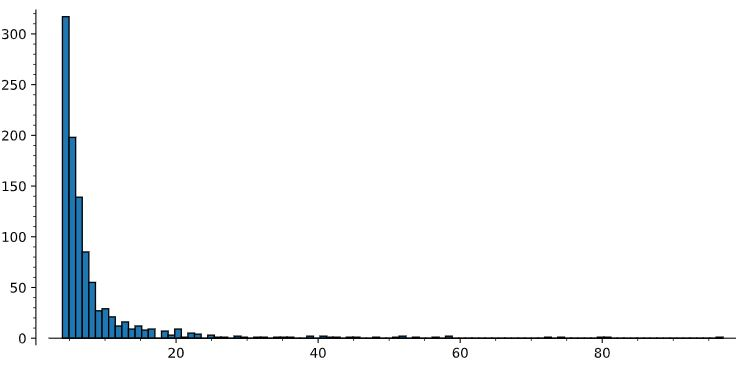
\includegraphics[width=0.9\textwidth]{degreepowerlawdist.jpg}
\caption{Sample degree distribution of a social network}\label{21p1}
\end{center}

\end{figure}
\begin{newpage}
\end{newpage}
 
Rishnak nodded and said, ``Yes, these individuals are sometimes referred to as hubs.''
 
Thinking about Erd\H{o}s again, Ajur remembered the Erd\H{o}s--R\'enyi model for generating random graphs. He asked, ``Do the Erd\H{o}s--R\'enyi graphs have a uniform degree distribution---I mean all of the vertices have roughly the same degrees?''

Rishnak smiled and said, ``Let me try to explore that further with an example using Facebook. A Facebook graph consists of users as vertices and edges between two users if they are friends of one another---and remember, in Facebook, friendship is a symmetric relationship. It has been found that the average number of Facebook friends per user, which is therefore the average degree of a vertex, is~300 and the median degree is~200.''

Ajur asked, ``How big is the Facebook graph? It must be humongous.''

Rishnak said, ``The Facebook graph has approximately two billion vertices---many of these vertices could be fake users or groups. With a median degree of~200, that means that one billion users have less than~200 friends.''

Ajur raised his eyebrows. He said, ``Wow, that's quite a long tail.''

Rishnak smiled, happy to see Ajur put the various pieces of the puzzle together. He continued, ``And Facebook restricts the maximum number of friends one can have to~5000. According to sociologists, a person can actually be close to at most~150 friends, which tells you something about how close friendships are in Facebook.''

Ajur laughed.

Rishnak continued, ``Also, the Facebook graph has an average separation or diameter of only~3.74.\footnote{\url{https://research.fb.com/blog/2016/02/three-and-a-half-degrees-of-separation/}} There is a well-known Facebook paradox that states that, on average, most people have fewer friends than their friends have. We can see this by studying this graph.'' Rishnak flashed his hands and a graph appeared [Figure~\ref{21g1}].

\begin{figure}
\begin{center}
\begin{tikzpicture}
  [scale=.6,auto=left,every node/.style={circle,fill=red!20}]
  \node (n1) at (1,7) {A};
  \node (n2) at (3,7)  {B};
  \node (n3) at (5,7)  {C};
  \node (n4) at (3,9)  {D};

  \foreach \from/\to in {n1/n2,n2/n3,n2/n4,n1/n4}
    \draw (\from) -- (\to);

\end{tikzpicture}
\caption{A graph that explains the Facebook friends paradox}\label{21g1}
\end{center}
\end{figure}

Rishnak said, ``In this graph, the average number of friends---in other words, the average degree---is~$\frac{2+2+3+1}{4}=2$.  Person~$A$ sees that~$D$ has two friends and~$B$ has three friends. Person~$B$ sees that~$A$ and~$D$ both have two friends and~$C$ has only one friend. Person~$C$ sees that~$B$ has three friends. And person~$D$ sees that~$A$ has two friends and~$B$ has three friends. Therefore, the average number of friends one sees is~$\frac{2+3+2+2+1+3+2+3}{8}=2.25$.''

Ajur frowned at this result.

Rishnak continued, ``This is in contradiction to the common belief that one has more friends than their friends have!''

Ajur protested, saying, ``That doesn't make any sense.''

Rishnak laughed and mentioned that there was a nice mathematical explanation for this phenomenon---and that Ajur should discover it on his own.

Kinaja, a glowing white ghost, suddenly appeared. She had been listening to Rishnak go on and on about social networks. She glided in to join them and said, ``I think that virtual social networks, being unregulated, cause a lot of harm---and here are three reasons why:
\begin{enumerate}
    \item Users can too easily be bullied.
    \item Bots and trolls pretend to be genuine users, but they propagate misinformation.
    \item One's private information too easily gets stolen or sold to advertisers.''
\end{enumerate}

Rishnak and Ajur both nodded in agreement.

\subsection*{Question for the nineteenth day}
Rishnak said, ``Ajur, we have come to the nineteenth day. Here is your question. Does the Facebook paradox still hold for a regular graph of degree~3 with 10 vertices?''

\textit{Before you turn the page, try to come up with an answer of your own!}

\newpage
\subsection*{Answer for the nineteenth day}
Ajur worked this problem out by thinking aloud. He said, ``If the degree is~3, then each person will have three friends, but the average number of friends one sees is~$\frac{(3+3+3)*10}{30}=3$. Therefore, for this graph, there will be no paradox.''

Rishnak said, ``Good, Ajur. And note that most real social networks are not regular, so most social networks do see this paradox.''

That was a good place to stop the discussion for the night.

\chapter{Instant Insanity Puzzle}

Rishnak was examining the headstones of some of the graves. He saw a headstone with a name Schossow \footnote{ Schossow got a patent for proposing this puzzle in 1899. \url{https://patents.google.com/patent/US646463A/en} }  in a grave. That brought him memories of the puzzle called the Great Tantalizer (also known as Instant Insanity). Schossow's puzzle had card suits (Hearts, Diamonds, Clubs and Spades) marked in each face. Frank Armbruster made a variation of this puzzle with colors instead of suits and that puzzle is called Instant Insanity Puzzle.
Rishnak thought that was a great puzzle to tell Ajur as this puzzle had a nice graph theoretic solution. As Rishnak was thinking, Ajur and Jura walked by. Rishnak told Ajur that he was going to talk about a puzzle which has a short solution using graph theory or a long solution using a search technique. The puzzle consists of four cubes with each face colored as shown in Figure \ref{22p1}. 
\begin{figure}
\begin{center}
\begin{tikzpicture}
[scale=.9]
%First Cube
\fill [red] (0.0,0.0) rectangle (0.5,0.5);
\fill [yellow] (0.5,0.0) rectangle (1.0,0.5);
\fill [green] (1.0,0.0) rectangle (1.5,0.5);
\fill [blue] (1.5,0.0) rectangle (2.0,0.5);
\fill [red] (0.5,-0.5) rectangle (1.0,0.0);
\fill [red] (0.5,0.5) rectangle (1.0,1.0);
%Second Cube
\fill [red] (3.0,0.0) rectangle (3.5,0.5);
\fill [yellow] (3.5,0.0) rectangle (4.0,0.5);
\fill [blue] (4.0,0.0) rectangle (4.5,0.5);
\fill [green] (4.5,0.0) rectangle (5.0,0.5);
\fill [yellow] (3.5,-0.5) rectangle (4.0,0.0);
\fill [red] (3.5,0.5) rectangle (4.0,1.0);
%Third  Cube
\fill [blue] (6.0,0.0) rectangle (6.5,0.5);
\fill [blue] (6.5,0.0) rectangle (7.0,0.5);
\fill [red] (7.0,0.0) rectangle (7.5,0.5);
\fill [yellow] (7.5,0.0) rectangle (8.0,0.5);
\fill [green] (6.5,-0.5) rectangle (7.0,0.0);
\fill [green] (6.5,0.5) rectangle (7.0,1.0);
%Fourth Cube
\fill [blue] (9.0,0.0) rectangle (9.5,0.5);
\fill [yellow] (9.5,0.0) rectangle (10.0,0.5);
\fill [red] (10.0,0.0) rectangle (10.5,0.5);
\fill [green] (10.5,0.0) rectangle (11.0,0.5);
\fill [yellow] (9.5,-0.5) rectangle (10.0,0.0);
\fill [blue] (9.5,0.5) rectangle (10.0,1.0);
\end{tikzpicture}
\caption{ Four Cubes}\label{22p1}
\end{center}
\end{figure}

The problem is to stack the four cubes vertically (in a column) so that all the cubes in each side (left, right, front and back) have distinct colors.
\begin{figure}
\begin{center}
\begin{tikzpicture}
\coordinate (O) at (0,0,0);
\coordinate (A) at (0,0.5,0);
\coordinate (B) at (0,0.5,0.5);
\coordinate (C) at (0,0,0.5);
\coordinate (D) at (0.5,0,0);
\coordinate (E) at (0.5,0.5,0);
\coordinate (F) at (0.5,0.5,0.5);
\coordinate (G) at (0.5,0,0.5);

\draw[black,fill=yellow] (O) -- (C) -- (G) -- (D) -- cycle;% Bottom Face
\draw[black,fill=blue] (O) -- (A) -- (E) -- (D) -- cycle;% Back Face
\draw[black,fill=blue] (O) -- (A) -- (B) -- (C) -- cycle;% Left Face
\draw[black,fill=red,opacity=0.7] (D) -- (E) -- (F) -- (G) --cycle;% Right Face
\draw[black,fill=yellow,opacity=0.7] (C) -- (B) -- (F) -- (G) --cycle;% Front Face
\draw[black,fill=green,opacity=0.7] (A) -- (B) -- (F) -- (E) -- cycle;% Top Face
\coordinate (OO) at (0,-0.5,0);
\coordinate (AA) at (0,0,0);
\coordinate (BB) at (0,0,0.5);
\coordinate (CC) at (0,-0.5,0.5);
\coordinate (DD) at (0.5,-0.5,0);
\coordinate (EE) at (0.5,0,0);
\coordinate (FF) at (0.5,0,0.5);
\coordinate (GG) at (0.5,-0.5,0.5);

\draw[black,fill=yellow] (OO) -- (CC) -- (GG) -- (DD) -- cycle;% Bottom Face
\draw[black,fill=red] (OO) -- (AA) -- (EE) -- (DD) -- cycle;% Back Face
\draw[black,fill=red] (OO) -- (AA) -- (BB) -- (CC) -- cycle;% Left Face
\draw[black,fill=green,opacity=0.7] (DD) -- (EE) -- (FF) -- (GG) --cycle;% Right Face
\draw[black,fill=red,opacity=0.7] (CC) -- (BB) -- (FF) -- (GG) --cycle;% Front Face
\draw[black,fill=blue,opacity=0.7] (AA) -- (BB) -- (FF) -- (EE) -- cycle;% Top Face
%% Following is for debugging purposes so you can see where the points are
%% These are last so that they show up on top
%\foreach \xy in {O, A, B, C, D, E, F, G}{
%    \node at (\xy) {\xy};
%}
\end{tikzpicture}
\caption{ Cube 4 on top of Cube 1 all faces have distinct colors}\label{22p2}
\end{center}
\end{figure}

We have illustrated with two cubes Cube number 4 sitting on top of Cube number 1 in Figure \ref{22p2}

Rishnak said that we consider three opposite faces of each cube. There are four colors Red, Yellow, Green and Blue. They form the vertices. Two vertices (colors) are adjacent if they form the opposite sides of the same cube. For example the following graph represents the first cube Figure \ref{22g1}.  

\begin{figure}[h]
\begin{center}
\begin{tikzpicture}
  [scale=.4,auto=left,every node/.style={circle}]
\node (n1)[fill=blue!50] at (4,4) {3};
  \node (n2)[fill=green!50] at (0,0)  {1};
  \node (n3)[fill=red!50] at (4,0)  {2};
  \node (n4)[fill=yellow!50] at (0,4)  {4};;
 \foreach \from/\to in {n3/n2,n1/n4}
    \draw[cyan,thick] (\from) -- (\to);
  \draw[cyan,thick]
  (n3) to[out=210,in=330,looseness=4] (n3);
\end{tikzpicture}
\caption{ Graph for Cube 1}\label{22g1}
\end{center}
\end{figure}

Similarly we can draw the graphs for each of the cubes Figures \ref{22g2}, \ref{22g3} and \ref{22g4}.

\begin{figure}[h]
\begin{center}
\begin{tikzpicture}
  [scale=.4,auto=left,every node/.style={circle}]
 \node (n1)[fill=blue!50] at (4,4) {3};
  \node (n2)[fill=green!50] at (0,0)  {1};
  \node (n3)[fill=red!50] at (4,0)  {2};
  \node (n4)[fill=yellow!50] at (0,4)  {4};

 \foreach \from/\to in {n3/n1,n3/n4,n2/n4}
    \draw[orange,thick] (\from) -- (\to);
\end{tikzpicture}
\caption{ Graph for Cube 2}\label{22g2}
\end{center}
\end{figure}

\begin{figure}[h]
\begin{center}
\begin{tikzpicture}
  [scale=.4,auto=left,every node/.style={circle}]
\node (n1)[fill=blue!50] at (4,4) {3};
  \node (n2)[fill=green!50] at (0,0)  {1};
  \node (n3)[fill=red!50] at (4,0)  {2};
  \node (n4)[fill=yellow!50] at (0,4)  {4};

 \foreach \from/\to in {n3/n1,n1/n4}
    \draw[black,thick] (\from) -- (\to);
     \draw[black,thick]
  (n2) to[out=210,in=330,looseness=4] (n2);
\end{tikzpicture}
\caption{ Graph for Cube 3}\label{22g3}
\end{center}
\end{figure}

\begin{figure}[h]
\begin{center}
\begin{tikzpicture}
  [scale=.4,auto=left,every node/.style={circle}]
\node (n1)[fill=blue!50] at (4,4) {3};
  \node (n2)[fill=green!50] at (0,0)  {1};
  \node (n3)[fill=red!50] at (4,0)  {2};
  \node (n4)[fill=yellow!50] at (0,4)  {4};
 \foreach \from/\to in {n3/n1,n1/n4,n2/n4}
    \draw[purple,thick] (\from) -- (\to);

\end{tikzpicture}
\caption{ Graph for Cube 4}\label{22g4}
\end{center}
\end{figure}

Now combining all these graphs in a single graph, we get a graph (looks complicated) Figure \ref{22g5}.

\begin{figure}[h]
\begin{center}
\begin{tikzpicture}
  [scale=.8,auto=left,every node/.style={circle}]
\node (n1)[fill=blue!50] at (4,4) {3};
  \node (n2)[fill=green!50] at (0,0)  {1};
  \node (n3)[fill=red!50] at (4,0)  {2};
  \node (n4)[fill=yellow!50] at (0,4)  {4};

 \foreach \from/\to in {n3/n2,n1/n4}
    \draw[cyan,thick] (\from) -- (\to);
  \draw[cyan,thick]
  (n3) to[out=210,in=330,looseness=4] (n3);
 \foreach \from/\to in {n3/n1,n3/n4,n2/n4}
    \draw[orange,thick] (\from) -- (\to); 

   
\end{tikzpicture}
\caption{ Graph for all the cubes}\label{22g5}
\end{center}
\end{figure}


\chapter{Conclusion}
Rishnak used to teach at a college in Royt. He was such a mean teacher that his students landed a curse on him such that he would remain a ghost until a student whom he teaches appreciates his teaching. Shortly after Ajur thanked Rishnak, Rishnak was released from his curse. He could now join his own ancestors in the other world. Rishnak was also happy that young Ajur was not afraid of failure and instead persevered to understand and solve all of the hard problems he faced.

%\chapter{Puzzle 5}
%\chapter{Puzzle 6}
%\chapter{Puzzle 7}
%\chapter{Puzzle 8}
%\chapter{Puzzle 9}
%\chapter{Puzzle 10}
%\chapter{Puzzle 11}
%\chapter{Puzzle 12}
%\chapter{Puzzle 13}
%\chapter{Puzzle 14}
%\chapter{Puzzle 15}
%\chapter{Puzzle 16}
%\chapter{Puzzle 17}
%\chapter{Puzzle 18}
%\chapter{Puzzle 19}
%\chapter{Puzzle 20}
%\chapter{Puzzle 21}
%\chapter{Puzzle 22}
%\chapter{Puzzle 23}
%\chapter{Puzzle 24}
%\chapter{Puzzle 25}



% Once upon a time\ldots This document shows how you can get ePub-like formatting in \LaTeX{} with the \verb|memoir| document class. You can't yet export directly to ePub from writeLaTeX, but you can download the source and run it through a format conversion tool, such as \verb|htlatex| to get HTML, and then go from HTML to ePub with a tool like Sigil or Calibre. See \url{http://tex.stackexchange.com/questions/16569} for more advice. And they lived happily ever after.

%\lipsum

\end{document}